% Options for packages loaded elsewhere
% Options for packages loaded elsewhere
\PassOptionsToPackage{unicode}{hyperref}
\PassOptionsToPackage{hyphens}{url}
\PassOptionsToPackage{dvipsnames,svgnames,x11names}{xcolor}
%
\documentclass[
  letterpaper,
  DIV=11,
  numbers=noendperiod]{scrreprt}
\usepackage{xcolor}
\usepackage{amsmath,amssymb}
\setcounter{secnumdepth}{5}
\usepackage{iftex}
\ifPDFTeX
  \usepackage[T1]{fontenc}
  \usepackage[utf8]{inputenc}
  \usepackage{textcomp} % provide euro and other symbols
\else % if luatex or xetex
  \usepackage{unicode-math} % this also loads fontspec
  \defaultfontfeatures{Scale=MatchLowercase}
  \defaultfontfeatures[\rmfamily]{Ligatures=TeX,Scale=1}
\fi
\usepackage{lmodern}
\ifPDFTeX\else
  % xetex/luatex font selection
\fi
% Use upquote if available, for straight quotes in verbatim environments
\IfFileExists{upquote.sty}{\usepackage{upquote}}{}
\IfFileExists{microtype.sty}{% use microtype if available
  \usepackage[]{microtype}
  \UseMicrotypeSet[protrusion]{basicmath} % disable protrusion for tt fonts
}{}
\makeatletter
\@ifundefined{KOMAClassName}{% if non-KOMA class
  \IfFileExists{parskip.sty}{%
    \usepackage{parskip}
  }{% else
    \setlength{\parindent}{0pt}
    \setlength{\parskip}{6pt plus 2pt minus 1pt}}
}{% if KOMA class
  \KOMAoptions{parskip=half}}
\makeatother
% Make \paragraph and \subparagraph free-standing
\makeatletter
\ifx\paragraph\undefined\else
  \let\oldparagraph\paragraph
  \renewcommand{\paragraph}{
    \@ifstar
      \xxxParagraphStar
      \xxxParagraphNoStar
  }
  \newcommand{\xxxParagraphStar}[1]{\oldparagraph*{#1}\mbox{}}
  \newcommand{\xxxParagraphNoStar}[1]{\oldparagraph{#1}\mbox{}}
\fi
\ifx\subparagraph\undefined\else
  \let\oldsubparagraph\subparagraph
  \renewcommand{\subparagraph}{
    \@ifstar
      \xxxSubParagraphStar
      \xxxSubParagraphNoStar
  }
  \newcommand{\xxxSubParagraphStar}[1]{\oldsubparagraph*{#1}\mbox{}}
  \newcommand{\xxxSubParagraphNoStar}[1]{\oldsubparagraph{#1}\mbox{}}
\fi
\makeatother

\usepackage{color}
\usepackage{fancyvrb}
\newcommand{\VerbBar}{|}
\newcommand{\VERB}{\Verb[commandchars=\\\{\}]}
\DefineVerbatimEnvironment{Highlighting}{Verbatim}{commandchars=\\\{\}}
% Add ',fontsize=\small' for more characters per line
\usepackage{framed}
\definecolor{shadecolor}{RGB}{241,243,245}
\newenvironment{Shaded}{\begin{snugshade}}{\end{snugshade}}
\newcommand{\AlertTok}[1]{\textcolor[rgb]{0.68,0.00,0.00}{#1}}
\newcommand{\AnnotationTok}[1]{\textcolor[rgb]{0.37,0.37,0.37}{#1}}
\newcommand{\AttributeTok}[1]{\textcolor[rgb]{0.40,0.45,0.13}{#1}}
\newcommand{\BaseNTok}[1]{\textcolor[rgb]{0.68,0.00,0.00}{#1}}
\newcommand{\BuiltInTok}[1]{\textcolor[rgb]{0.00,0.23,0.31}{#1}}
\newcommand{\CharTok}[1]{\textcolor[rgb]{0.13,0.47,0.30}{#1}}
\newcommand{\CommentTok}[1]{\textcolor[rgb]{0.37,0.37,0.37}{#1}}
\newcommand{\CommentVarTok}[1]{\textcolor[rgb]{0.37,0.37,0.37}{\textit{#1}}}
\newcommand{\ConstantTok}[1]{\textcolor[rgb]{0.56,0.35,0.01}{#1}}
\newcommand{\ControlFlowTok}[1]{\textcolor[rgb]{0.00,0.23,0.31}{\textbf{#1}}}
\newcommand{\DataTypeTok}[1]{\textcolor[rgb]{0.68,0.00,0.00}{#1}}
\newcommand{\DecValTok}[1]{\textcolor[rgb]{0.68,0.00,0.00}{#1}}
\newcommand{\DocumentationTok}[1]{\textcolor[rgb]{0.37,0.37,0.37}{\textit{#1}}}
\newcommand{\ErrorTok}[1]{\textcolor[rgb]{0.68,0.00,0.00}{#1}}
\newcommand{\ExtensionTok}[1]{\textcolor[rgb]{0.00,0.23,0.31}{#1}}
\newcommand{\FloatTok}[1]{\textcolor[rgb]{0.68,0.00,0.00}{#1}}
\newcommand{\FunctionTok}[1]{\textcolor[rgb]{0.28,0.35,0.67}{#1}}
\newcommand{\ImportTok}[1]{\textcolor[rgb]{0.00,0.46,0.62}{#1}}
\newcommand{\InformationTok}[1]{\textcolor[rgb]{0.37,0.37,0.37}{#1}}
\newcommand{\KeywordTok}[1]{\textcolor[rgb]{0.00,0.23,0.31}{\textbf{#1}}}
\newcommand{\NormalTok}[1]{\textcolor[rgb]{0.00,0.23,0.31}{#1}}
\newcommand{\OperatorTok}[1]{\textcolor[rgb]{0.37,0.37,0.37}{#1}}
\newcommand{\OtherTok}[1]{\textcolor[rgb]{0.00,0.23,0.31}{#1}}
\newcommand{\PreprocessorTok}[1]{\textcolor[rgb]{0.68,0.00,0.00}{#1}}
\newcommand{\RegionMarkerTok}[1]{\textcolor[rgb]{0.00,0.23,0.31}{#1}}
\newcommand{\SpecialCharTok}[1]{\textcolor[rgb]{0.37,0.37,0.37}{#1}}
\newcommand{\SpecialStringTok}[1]{\textcolor[rgb]{0.13,0.47,0.30}{#1}}
\newcommand{\StringTok}[1]{\textcolor[rgb]{0.13,0.47,0.30}{#1}}
\newcommand{\VariableTok}[1]{\textcolor[rgb]{0.07,0.07,0.07}{#1}}
\newcommand{\VerbatimStringTok}[1]{\textcolor[rgb]{0.13,0.47,0.30}{#1}}
\newcommand{\WarningTok}[1]{\textcolor[rgb]{0.37,0.37,0.37}{\textit{#1}}}

\usepackage{longtable,booktabs,array}
\newcounter{none} % for unnumbered tables
\usepackage{calc} % for calculating minipage widths
% Correct order of tables after \paragraph or \subparagraph
\usepackage{etoolbox}
\makeatletter
\patchcmd\longtable{\par}{\if@noskipsec\mbox{}\fi\par}{}{}
\makeatother
% Allow footnotes in longtable head/foot
\IfFileExists{footnotehyper.sty}{\usepackage{footnotehyper}}{\usepackage{footnote}}
\makesavenoteenv{longtable}
\usepackage{graphicx}
\makeatletter
\newsavebox\pandoc@box
\newcommand*\pandocbounded[1]{% scales image to fit in text height/width
  \sbox\pandoc@box{#1}%
  \Gscale@div\@tempa{\textheight}{\dimexpr\ht\pandoc@box+\dp\pandoc@box\relax}%
  \Gscale@div\@tempb{\linewidth}{\wd\pandoc@box}%
  \ifdim\@tempb\p@<\@tempa\p@\let\@tempa\@tempb\fi% select the smaller of both
  \ifdim\@tempa\p@<\p@\scalebox{\@tempa}{\usebox\pandoc@box}%
  \else\usebox{\pandoc@box}%
  \fi%
}
% Set default figure placement to htbp
\def\fps@figure{htbp}
\makeatother

\ifLuaTeX
  \usepackage{luacolor}
  \usepackage[soul]{lua-ul}
\else
  \usepackage{soul}
\fi




\setlength{\emergencystretch}{3em} % prevent overfull lines

\providecommand{\tightlist}{%
  \setlength{\itemsep}{0pt}\setlength{\parskip}{0pt}}



 


\KOMAoption{captions}{tableheading}
\makeatletter
\@ifpackageloaded{bookmark}{}{\usepackage{bookmark}}
\makeatother
\makeatletter
\@ifpackageloaded{caption}{}{\usepackage{caption}}
\AtBeginDocument{%
\ifdefined\contentsname
  \renewcommand*\contentsname{Table of contents}
\else
  \newcommand\contentsname{Table of contents}
\fi
\ifdefined\listfigurename
  \renewcommand*\listfigurename{List of Figures}
\else
  \newcommand\listfigurename{List of Figures}
\fi
\ifdefined\listtablename
  \renewcommand*\listtablename{List of Tables}
\else
  \newcommand\listtablename{List of Tables}
\fi
\ifdefined\figurename
  \renewcommand*\figurename{Figure}
\else
  \newcommand\figurename{Figure}
\fi
\ifdefined\tablename
  \renewcommand*\tablename{Table}
\else
  \newcommand\tablename{Table}
\fi
}
\@ifpackageloaded{float}{}{\usepackage{float}}
\floatstyle{ruled}
\@ifundefined{c@chapter}{\newfloat{codelisting}{h}{lop}}{\newfloat{codelisting}{h}{lop}[chapter]}
\floatname{codelisting}{Listing}
\newcommand*\listoflistings{\listof{codelisting}{List of Listings}}
\makeatother
\makeatletter
\makeatother
\makeatletter
\@ifpackageloaded{caption}{}{\usepackage{caption}}
\@ifpackageloaded{subcaption}{}{\usepackage{subcaption}}
\makeatother
\usepackage{bookmark}
\IfFileExists{xurl.sty}{\usepackage{xurl}}{} % add URL line breaks if available
\urlstyle{same}
% fallback for those not using the hyperref driver hyperxmp:
\makeatletter
\@ifundefined{xmpquote}{\newcommand{\xmpquote}[1]{#1}}{}
\makeatother
\hypersetup{
  pdftitle={quantcrim},
  pdfauthor={Joost Jansen; Gijs Custers},
  colorlinks=true,
  linkcolor={blue},
  filecolor={Maroon},
  citecolor={Blue},
  urlcolor={Blue},
  pdfcreator={LaTeX via pandoc}}


\title{quantcrim}
\usepackage{etoolbox}
\makeatletter
\providecommand{\subtitle}[1]{% add subtitle to \maketitle
  \apptocmd{\@title}{\par {\large #1 \par}}{}{}
}
\makeatother
\subtitle{Een open-web handboek voor kwantitatief criminologisch
onderzoek}
\author{Joost Jansen \and Gijs Custers}
\date{2026-10-27}
\begin{document}
\maketitle

\renewcommand*\contentsname{Table of contents}
{
\setcounter{tocdepth}{2}
\tableofcontents
}

\bookmarksetup{startatroot}

\chapter{Voorwoord}\label{voorwoord}

\bookmarksetup{startatroot}

\chapter*{Voorwoord}\label{voorwoord-1}
\addcontentsline{toc}{chapter}{Voorwoord}

\markboth{Voorwoord}{Voorwoord}

Welkom bij het \href{quantcrim.pdf}{quantcrim handboek} Criminologie.
Hier ga je leren hoe je kwantitatieve data kan analyseren met R. Het
boek is ontworpen en beschikbaar gesteld door docenten en onderzoekers
van de opleiding Criminologie aan de Erasmus Universiteit. Het boek is
bedoeld voor zowel bachelor- als masterstudenten.

Hieronder vind je een voorbeeld van hoe makkelijk het is om data in te
laden, een regressiemodel te schatten en de resultaten ervan te
presenteren in een plot.\footnote{We gaan in een later hoofdstuk zien
  wat een regressiemodel precies is.}

\begin{Shaded}
\begin{Highlighting}[]
\CommentTok{\# test}
\end{Highlighting}
\end{Shaded}

Stuk tekst van McElrath over waarom werken met R en code

\section{Voor we verder gaan..}\label{voor-we-verder-gaan..}

We hopen dat je dit boek handig vindt om mee te werken. In het kader van
Open Science hebben we geprobeerd dit boek volledig transparant en
reproduceerbaar te ontwikkelen. De broncode is beschikbaar via
\href{https://github.com/joostjansen/QuantCrim}{https://github.com/joostjansen/quantcrim}.
Als je vragen, suggesties of aanpassingen hebt, aarzel niet deze te
stellen.\footnote{Het beste is om dit via GitHub te doen in onze
  Repository.}

\bookmarksetup{startatroot}

\chapter{Voorbereiding}\label{voorbereiding}

\bookmarksetup{startatroot}

\chapter*{Voorbereidingen}\label{voorbereidingen}
\addcontentsline{toc}{chapter}{Voorbereidingen}

\markboth{Voorbereidingen}{Voorbereidingen}

Voor we tijdens de lessen aan de slag kunnen met het verrichten van
kwantitatief onderzoek, moet de vereiste software geinstalleerd worden.
We gaan werken met R (spreek uit op z'n Engels). R is een
programmeertaal die veel statistici gebruiken om hun analyses mee te
doen. De omgeving waarin je met R kan werken, heet RStudio. Zowel R als
RStudio moeten apart geinstalleerd worden. Je vindt de installatielinks
hieronder:

\begin{enumerate}
\def\labelenumi{\arabic{enumi}.}
\tightlist
\item
  \href{https://cran.r-project.org/}{R}
\item
  \href{https://docs.posit.co/ide/user/\#rstudio-ide-oss-downloads}{RStudio}
\end{enumerate}

Na installatie van de benodigde software moeten we R gereed maken door
de juiste packages (ook wel: libraries) te installeren. Veel
databewerkingen en analyses vergen namelijk speciaal daarvoor software.
Een package waarmee je mooie visualisaties kan maken van je data heet
bijvoorbeeld ggplot. Je installeert zo'n package door RStudio te openen
en in je console de volgende code te typen en dan te `runnen':

\begin{Shaded}
\begin{Highlighting}[]
\CommentTok{\# install.packages("ggplot2")}
\end{Highlighting}
\end{Shaded}

Als je het package geinstalleerd hebt (eenmalig) laad je in het vervolg
aan het begin van elke sessie het package in. Let op: in tegenstelling
tot bij het installeren van een package, gebruik je bij het laden ervan
geen aanhalingstekens. R is zeer gevoelig voor het verkeerd gebruik van
leestekens. Wees daar dus scherp op.

\begin{Shaded}
\begin{Highlighting}[]
\FunctionTok{library}\NormalTok{(ggplot2)}
\end{Highlighting}
\end{Shaded}

Hieronder vind je een lijst met alle packages die je tijdens dit vak
nodig hebt.

\begin{Shaded}
\begin{Highlighting}[]
\CommentTok{\# }
\CommentTok{\# install.packages()}
\CommentTok{\# install.packages()}

\CommentTok{\# laden packages}
\FunctionTok{library}\NormalTok{(readr)}
\FunctionTok{library}\NormalTok{(ggplot2)}
\FunctionTok{library}\NormalTok{(tidyverse)}
\end{Highlighting}
\end{Shaded}

\part{Data beschrijven}

\chapter{Data}\label{data}

\section{\texorpdfstring{\textbf{Wat zijn
data?}}{Wat zijn data?}}\label{sec-data}

In de criminologie zijn we geïnteresseerd in diverse vragen die we
kunnen beantwoorden aan de hand van statistisch onderzoek. Denk aan de
volgende vragen:

\begin{itemize}
\tightlist
\item
  Hoeveel inbraken vinden er jaarlijks plaats in Kralingen?
\item
  Wat is het gemiddelde geldbedrag waarvoor Nederlandse banken hebben
  geschikt in witwaszaken in 2025?
\item
  Hoeveel misdaadjournalisten zijn er vermoord het afgelopen decennium?
\item
  Wat is de associatie tussen drugsverslaving en delinquentie?
\item
  In hoeverre leidt seksuele straatintimidatie tot het vermijden van
  bepaalde plekken?
\end{itemize}

Om deze vragen te kunnen beantwoorden, werken we met \textbf{datasets}.
Een set is in de wiskunde een verzameling van dingen. Een dataset is dus
een verzameling van data. Het woord \textbf{data} is afkomstig uit het
Latijnse `datum' wat letterlijk `gegeven' betekent. Een dataset is dus
een verzameling gegevens. Dit kan gaan over gegevens van mensen
(bijvoorbeeld hun lengte of geslacht), maar bijvoorbeeld ook over andere
dingen zoals organisaties, steden of landen. Hetgene waar de data
informatie over verschaffen (mensen, organisaties, steden, landen)
noemen we de \textbf{analyse-eenheid}.

In deze cursus werken we steeds met dezelfde dataset. Dit is gebaseerd
op een onderzoek onder uitgaande jongeren,
\href{https://www.trimbos.nl/kennisbank/rapport-het-grote-uitgaansonderzoek-2023/}{Het
Grote Uitgaansonderzoek} van het \href{https://www.trimbos.nl/}{Trimbos
Instituut}. In dit onderzoek wordt onder andere gekeken hoe vaak
jongeren uitgaan, wat voor soort feesten en gelegenheden ze bezoeken,
wat voor middelen ze gebruiken (bijvoorbeeld alcohol of andere drugs) en
hoe ze denken over drugsgebruik. Om de data te verzamelen is een online
enquête afgenomen via een gerichte wervingscampagne.

Laten we eerst kijken hoe zo'n dataset eruitziet. Dat doen we met behulp
van R. Zoals aangegeven in de introductie van dit online boek, het is
niet erg als je nog niet snapt hoe dit werkt. Daarvoor volg je uiteraard
deze cursus :)

\begin{Shaded}
\begin{Highlighting}[]
\CommentTok{\# laden van de voorbeeld data}
\NormalTok{voorbeeld\_data }\OtherTok{\textless{}{-}} \FunctionTok{read\_rds}\NormalTok{(}\StringTok{"data/voorbeeld\_data.rds"}\NormalTok{)}

\CommentTok{\# data inspecteren}
\FunctionTok{head}\NormalTok{(voorbeeld\_data) }\CommentTok{\# head() voor bekijken bovenste rijen}
\end{Highlighting}
\end{Shaded}

\begin{verbatim}
  geslacht leeftijd opleidingsniveau alcohol_ooit alcohol_laatste_jaar
1    vrouw       30           midden           ja                   ja
2      man       21             laag           ja                   ja
3    vrouw       35           midden           ja                  nee
4      man       16             hoog           ja                   ja
5      man       26             <NA>           ja                   ja
6    vrouw       18             laag           ja                   ja
\end{verbatim}

Hierboven staat een `sneak preview' van de dataset. Waar kijken we nu
eigenlijk naar? De dataset verschaft informatie die we verzameld hebben
over jongeren die hebben meegedaan aan de enquête. Elke rij
representeert een \textbf{respondent}: een jongere die de enquête heeft
ingevuld. De rijen zijn onze \textbf{observaties}.

Elke kolom bevat de waarde van die respondent met betrekking tot een
kenmerk, de waarde die hoort bij een antwoord dat een respondent gaf op
een in de enquête gestelde vraag. De waarden van respondenten op
kenmerken kunnen variëren van respondent tot respondent. Niet iedereen
is even oud, gebruikt even vaak drugs, heeft dezelfde opleiding etc. De
variatie in een bepaald kenmerk meten we met behulp van
\textbf{variabelen}. Deze zien we terug in de kolommen. De kern van
statistiek is dat we alle variatie in kenmerken gaan gebruiken om
onderzoeksvragen zoals die hierboven te kunnen beantwoorden.

We kunnen bijvoorbeeld zien dat de eerste respondent een vrouw is, 30
jaar oud, en een middelbaar opleidingsniveau heeft.

De vierde en vijfde kolom geven aan of iemand ooit alcohol heeft
gedronken of in het afgelopen jaar. De voorbeeld data toont dat vijf
respondenten het afgelopen jaar alcohol hebben gedronken en één
respondent niet.

\subsection{Missende waarden}\label{missende-waarden}

Wat je misschien ook is opgevallen, is dat in de vijfde rij bij
opleidingsniveau `NA' staat. Dit staat voor Not Available en geeft aan
dat er geen valide waarde is voor deze respondent op dit kenmerk. Van
deze persoon weten we het opleidingsniveau dus niet. Dit noemen we een
\textbf{missende waarde}.

Missende waarden komen vaak voor in onderzoek om diverse redenen. Zo
kunnen mensen een vraag verkeerd invullen, een vraag per ongeluk
overslaan, of een vraag niet willen beantwoorden. Dit laatste zien we
vaker bij gevoelige vragen, bijvoorbeeld over gedrag dat maatschappelijk
wordt afgekeurd (drugsgebruik!).

Missende waarden hoeven niet altijd een probleem te zijn. Dit hangt af
van de de aard van missende waarden en de hoeveelheid. In de practica
besteden we hier meer aandacht aan.

\chapter{Meetniveaus en
visualisaties}\label{meetniveaus-en-visualisaties}

Op de vorige pagina heb je gezien wat een dataset is, en dat deze
bestaat uit observaties (de rijen) en variabelen (de kolommen). In de
basis zijn er vier manieren om variabelen meetbaar te maken (ook wel:
operationaliseren). We noemen deze manieren \textbf{meetniveaus.} Elk
meetniveau verschaft een ander soort informatie. We bespreken hier de
vier meetniveaus en daarbij gaan we meteen in op hoe we de informatie
die de variabelen verschaffen het beste visueel kunnen presenteren.

Doorgaans maken we onderscheid tussen \textbf{kwalitatieve} en
\textbf{kwantitatieve} variabelen.

\section{Kwalitatieve variabelen}\label{kwalitatieve-variabelen}

Kwalitatieve variabelen bestaan uit categorieën die een kwalitatieve
eigenschap van een observatie beschrijven. Deze eigenschappen zijn niet
direct in cijfers uit te drukken, zoals bij kwantitatieve variabelen.
Een belangrijk aspect is dat de categorieën \emph{discreet} zijn: ze
moeten elkaar uitsluiten.

\subsection{Staafdiagram}\label{staafdiagram}

Laten we naar een voorbeeld kijken: geslacht. Stel dat we willen weten
hoeveel mannen, vrouwen of anders-identificerenden er in de dataset
zitten. Daarvoor kunnen we \textbf{staafdiagram} maken met
\emph{ggplot()}.

\begin{Shaded}
\begin{Highlighting}[]
\CommentTok{\# staafdiagram maken}
\FunctionTok{ggplot}\NormalTok{(data\_uitgaan, }\FunctionTok{aes}\NormalTok{(}\AttributeTok{x =}\NormalTok{ geslacht)) }\SpecialCharTok{+} \CommentTok{\# data en variabele selecteren}
  \FunctionTok{geom\_bar}\NormalTok{() }\CommentTok{\# staafdiagram}
\end{Highlighting}
\end{Shaded}

\pandocbounded{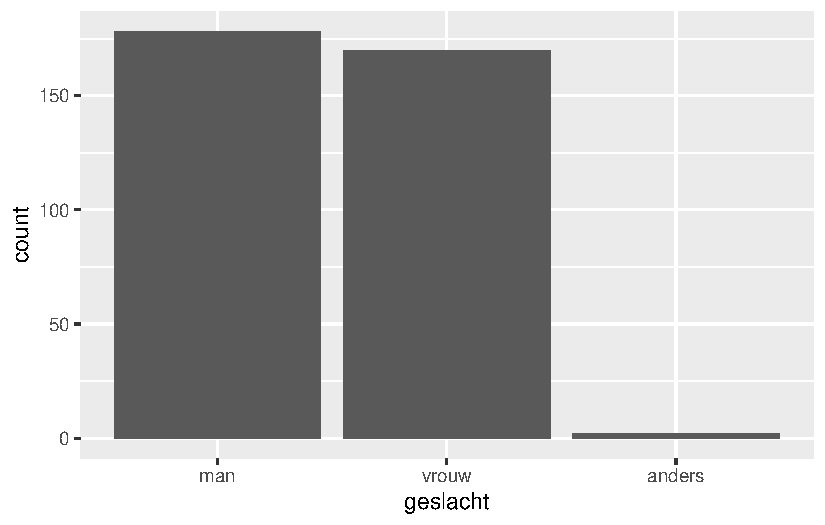
\includegraphics[keepaspectratio]{002-02-meetniveaus-visualisaties_files/figure-pdf/unnamed-chunk-2-1.pdf}}

De staafdiagram geeft een visuele presentatie van het aantal mannen,
vrouwen en anders-identificerenden in de dataset. Het mooie aan R is dat
we de figuur visueel nog wat aantrekkelijker kunnen maken. Hiermee ga je
meer oefenen tijdens de cursus.

\begin{Shaded}
\begin{Highlighting}[]
\CommentTok{\# staafdiagram met betere visualisatie}
\FunctionTok{ggplot}\NormalTok{(data\_uitgaan, }\FunctionTok{aes}\NormalTok{(}\AttributeTok{x =}\NormalTok{ geslacht)) }\SpecialCharTok{+}
  \FunctionTok{geom\_bar}\NormalTok{() }\SpecialCharTok{+}
  \FunctionTok{theme\_bw}\NormalTok{() }\SpecialCharTok{+} \CommentTok{\# witte achtergrond}
  \FunctionTok{ylab}\NormalTok{(}\StringTok{"aantal"}\NormalTok{)  }\CommentTok{\# label voor y{-}as}
\end{Highlighting}
\end{Shaded}

\pandocbounded{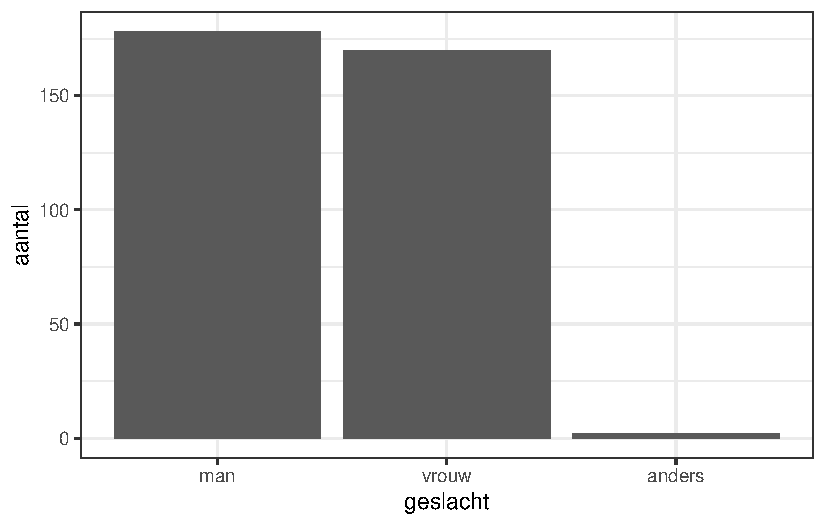
\includegraphics[keepaspectratio]{002-02-meetniveaus-visualisaties_files/figure-pdf/unnamed-chunk-3-1.pdf}}

De figuur heeft nu een witte achtergrond en de y-as heeft een
Nederlandstalig label.

\subsection{Simpele tabel}\label{simpele-tabel}

Als je wilt weten hoeveel respondenten er precies in elke categorie
zitten, kun je ook een simpele tabel maken met de functie
\emph{table()}.

\begin{Shaded}
\begin{Highlighting}[]
\CommentTok{\# tabel van geslacht}
\FunctionTok{table}\NormalTok{(data\_uitgaan}\SpecialCharTok{$}\NormalTok{geslacht)}
\end{Highlighting}
\end{Shaded}

\begin{verbatim}

   man  vrouw anders 
   178    170      2 
\end{verbatim}

De dataset bevat in totaal dus xxx mannen, xxx vrouwen en xxx in de
categorie ``anders''.

\subsection{Nominale variabele}\label{nominale-variabele}

Geslacht is een voorbeeld van een \textbf{nominale} variabele. Dit is
een kwalitatieve variabele waarin geen rangorde bestaat tussen de
categorieën. Mannen hebben niet intrinsiek meer waarde dan vrouwen, of
andersom. De variabele bestaat uit discrete categorieën die elkaar
uitsluiten, maar je kunt niet zeggen dat de ene categorie `hoger' of
`lager' is dan de ander.

\subsection{Taartdiagram}\label{taartdiagram}

Een andere manier om een nominale variabele te presenteren, is via een
\textbf{taartdiagram}. Een taartdiagram kan snel een overzicht geven van
de verhouding tussen categorieën binnen een bepaalde variabele.
Doorgaans werkt een taartdiagram het beste als er een beperkt aantal
categorieën zijn.

Hieronder staat een voorbeeld van taartdiagram van de variabele
manier\_verkrijgen\_drugs. Dit gaat over de wijze waarop uitgaande
jongeren meestal aan hun drugs komen.

\begin{Shaded}
\begin{Highlighting}[]
\CommentTok{\# samenvatten van de relevante data}
\NormalTok{drugs\_verkrijgen }\OtherTok{\textless{}{-}}\NormalTok{ data\_uitgaan }\SpecialCharTok{|\textgreater{}}
  \FunctionTok{filter}\NormalTok{(}\SpecialCharTok{!}\FunctionTok{is.na}\NormalTok{(manier\_verkrijgen\_drugs)) }\SpecialCharTok{|\textgreater{}} \CommentTok{\# missende waarden verwijderen}
  \FunctionTok{group\_by}\NormalTok{(manier\_verkrijgen\_drugs) }\SpecialCharTok{|\textgreater{}} \CommentTok{\# groeperen op variabele}
  \FunctionTok{summarise}\NormalTok{(}\AttributeTok{n =} \FunctionTok{n}\NormalTok{()) }\SpecialCharTok{|\textgreater{}} \CommentTok{\# aantal respondenten per categorie berekenen}
  \FunctionTok{mutate}\NormalTok{(}\AttributeTok{perc =} \FunctionTok{round}\NormalTok{(n}\SpecialCharTok{/}\FunctionTok{sum}\NormalTok{(n) }\SpecialCharTok{*} \DecValTok{100}\NormalTok{, }\DecValTok{1}\NormalTok{)) }\CommentTok{\# percentages berekenen en afronden op 1 decimaal}

\CommentTok{\# taartdiagram van hoe drugs worden verkregen}
\FunctionTok{ggplot}\NormalTok{(drugs\_verkrijgen, }\FunctionTok{aes}\NormalTok{(}\AttributeTok{x=} \StringTok{""}\NormalTok{, }\AttributeTok{y =}\NormalTok{ perc, }\AttributeTok{fill =}\NormalTok{ manier\_verkrijgen\_drugs)) }\SpecialCharTok{+} 
  \CommentTok{\# percentages (y) en categorieen (fill) selecteren}
  \FunctionTok{geom\_bar}\NormalTok{(}\AttributeTok{stat =} \StringTok{"identity"}\NormalTok{, }\AttributeTok{width =} \DecValTok{1}\NormalTok{) }\SpecialCharTok{+}
  \FunctionTok{coord\_polar}\NormalTok{(}\StringTok{"y"}\NormalTok{, }\AttributeTok{start =} \DecValTok{0}\NormalTok{) }\SpecialCharTok{+} \CommentTok{\# optie voor taartdiagram }
  \FunctionTok{theme\_void}\NormalTok{() }\CommentTok{\# achtergrond weghalen}
\end{Highlighting}
\end{Shaded}

\pandocbounded{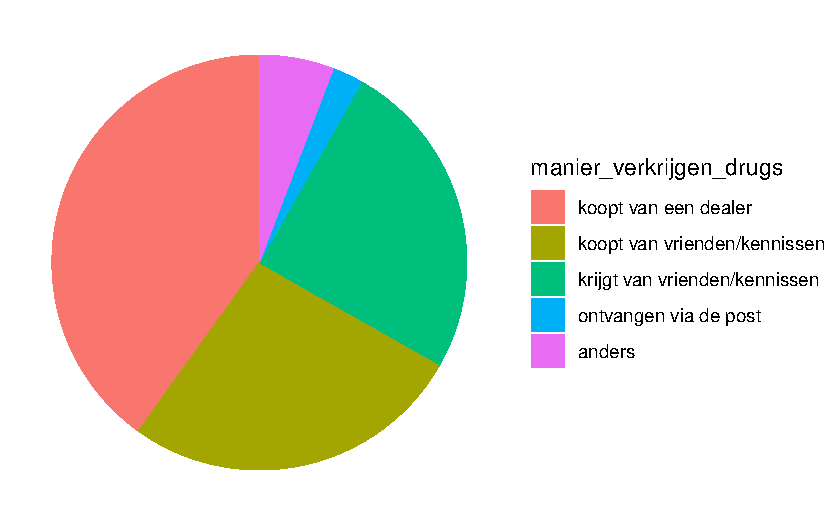
\includegraphics[keepaspectratio]{002-02-meetniveaus-visualisaties_files/figure-pdf/unnamed-chunk-5-1.pdf}}

Je kan zien dat er best wat regels code nodig zijn om deze taartdiagram
te maken. Hoe dat precies in zijn werk gaat, wat elke regel doet, gaan
we tijdens de practica behandelen.

De taartdiagram weergeeft het aandeel per categorie van hoe jongeren
doorgaans aan hun drugs komen. We kunnen de presentatie van de
taartdiagram echter nog verbeteren.

\begin{Shaded}
\begin{Highlighting}[]
\CommentTok{\# taartdiagram van hoe drugs worden verkregen}
\FunctionTok{ggplot}\NormalTok{(drugs\_verkrijgen, }\FunctionTok{aes}\NormalTok{(}\AttributeTok{x=} \StringTok{""}\NormalTok{, }\AttributeTok{y =}\NormalTok{ perc, }\AttributeTok{fill =}\NormalTok{ manier\_verkrijgen\_drugs)) }\SpecialCharTok{+} 
  \FunctionTok{geom\_bar}\NormalTok{(}\AttributeTok{stat =} \StringTok{"identity"}\NormalTok{, }\AttributeTok{width =} \DecValTok{1}\NormalTok{, }\AttributeTok{colour =} \StringTok{"white"}\NormalTok{) }\SpecialCharTok{+} \CommentTok{\# witte randen toevoegen}
  \FunctionTok{coord\_polar}\NormalTok{(}\StringTok{"y"}\NormalTok{, }\AttributeTok{start =} \DecValTok{0}\NormalTok{) }\SpecialCharTok{+}
  \FunctionTok{theme\_void}\NormalTok{() }\SpecialCharTok{+} 
  \FunctionTok{geom\_text}\NormalTok{(}\FunctionTok{aes}\NormalTok{(}\AttributeTok{label =}\NormalTok{ perc), }\AttributeTok{position =} \FunctionTok{position\_stack}\NormalTok{(}\AttributeTok{vjust =} \FloatTok{0.5}\NormalTok{)) }\SpecialCharTok{+} \CommentTok{\# percentages als labels toevoegen   }
  \FunctionTok{labs}\NormalTok{(}\AttributeTok{fill =} \StringTok{"Manieren van drugs verkrijgen (\%)"}\NormalTok{) }\CommentTok{\# titel voor legenda}
\end{Highlighting}
\end{Shaded}

\pandocbounded{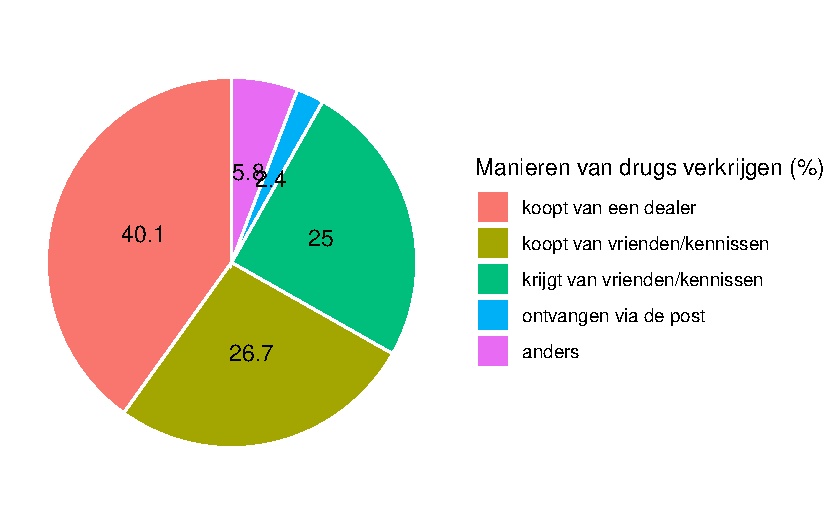
\includegraphics[keepaspectratio]{002-02-meetniveaus-visualisaties_files/figure-pdf/unnamed-chunk-6-1.pdf}}

We hebben nu een duidelijk inzicht in hoe jongeren die drugs gebruiken
hier aan komen. Zo zien we bijvoorbeeld dat ongeveer xx procent dit via
een dealer koopt, en ongeveer een kwart het koopt via vrienden/kennissen
en een kwart het van deze krijgt.

Dit toont meteen een relevante bevinding uit de literatuur over
drugsgebruik onder jongeren, namelijk dat de helft van de jongeren hun
drugs verkrijgen via ``\emph{sorting}'' (zie
\href{https://journals.sagepub.com/doi/10.1177/003803850203600408}{Parker
et al., 2002}). Dat wil zeggen, dat een bekende uit een vrienden- of
kennissenkring iemand van drugs voorziet eerder dan een dealer.

\subsection{Ordinale variabele}\label{ordinale-variabele}

Een kwalitatieve variabele waarbij er \emph{wel} een bepaalde rangorde
(hiërarchie) tussen de categorieën is, noemen we een \textbf{ordinale}
variabele.

Laten we weer naar een voorbeeld kijken. In de enquête is gevraagd hoe
jongeren hun eigen gezondheid over het algemeen beoordelen. Voor een
ordinale variabele maken we in principe altijd een staafdiagram.

\begin{Shaded}
\begin{Highlighting}[]
\CommentTok{\# staafdiagram van ervaren gezondheid}
\FunctionTok{ggplot}\NormalTok{(data\_uitgaan, }\FunctionTok{aes}\NormalTok{(}\AttributeTok{x =}\NormalTok{ ervaren\_gezondheid)) }\SpecialCharTok{+}
  \FunctionTok{geom\_bar}\NormalTok{() }\SpecialCharTok{+}
  \FunctionTok{theme\_bw}\NormalTok{() }\SpecialCharTok{+} 
  \FunctionTok{ylab}\NormalTok{(}\StringTok{"aantal"}\NormalTok{) }\SpecialCharTok{+}
  \FunctionTok{xlab}\NormalTok{ (}\StringTok{"ervaren gezondheid"}\NormalTok{)}
\end{Highlighting}
\end{Shaded}

\pandocbounded{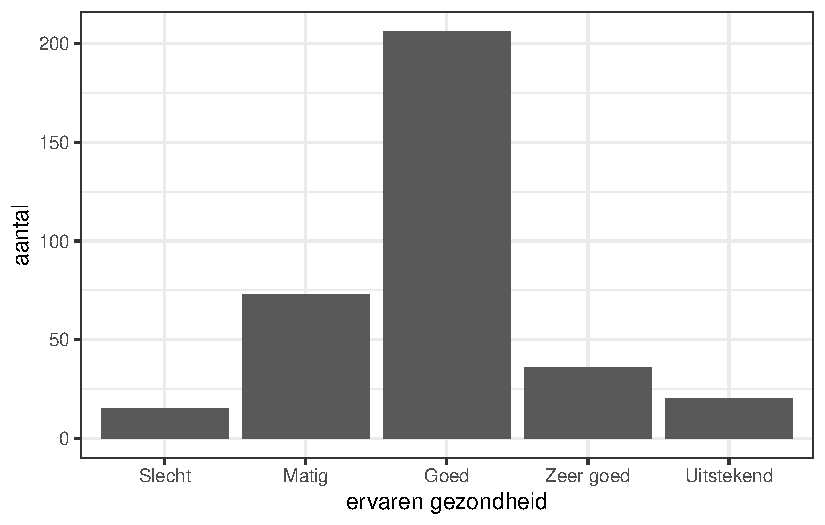
\includegraphics[keepaspectratio]{002-02-meetniveaus-visualisaties_files/figure-pdf/unnamed-chunk-7-1.pdf}}

De staafdiagram toont dat het grootste deel hun gezondheid als ``goed''
beoordeelt. Een relatief klein deel van de jongeren beoordeelt hun
gezondheid als ``matig'' of zelfs ``slecht''.

Dit voorbeeld illustreert een relevant kenmerk van ordinale variabelen:
er is een bepaalde rangorde tussen de categorieën, maar de afstand
ertussen is niet per se gelijk. Zo is de stap van ``matig'' naar
``goed'' bijvoorbeeld kwalitatief anders dan de stap van ``zeer goed''
naar ``uitstekend''. Hierin verschilt een ordinale variabele doorgaans
van een kwantitatieve variabele, bij de laatste is de afstand tussen
waarden (1-2-3 etc.) in principe altijd gelijk.

Bij een ordinale variable kan het echter ook zijn dat de afstand tussen
categorieën als gelijk wordt gezien. Als je bijvoorbeeld een antwoord op
een stelling meet met de volgende antwoordcategorieën:

\begin{itemize}
\tightlist
\item
  helemaal mee oneens
\item
  mee oneens
\item
  niet mee oneens / niet mee eens
\item
  mee eens
\item
  helemaal mee eens
\end{itemize}

Dan wordt vaak aangenomen dat de afstand tussen de categorieën gelijk
is. Zie verderop onder het kopje Section~\ref{sec-meetniveaubepalen}
meer uitleg hierover.

\section{Kwantitatieve variabelen}\label{kwantitatieve-variabelen}

Kwantitatieve variabelen zijn numeriek en bestaan dus uit cijfers. De
afstand tussen waarden is altijd gelijk en er zit een rangorde in.
Bijvoorbeeld bij een rapportcijfer van 1 t/m 10 is de afstand tussen 2
en 3 hetzelfde als de afstand tussen 7 en 8. Kwantitatieve variabelen
worden soms ook wel lineaire of continue variabelen genoemd.

\subsection{Interval en ratio variabelen}\label{sec-intervalratio}

Er zijn twee types kwantitatieve variabelen: \textbf{interval} en
\textbf{ratio}. Het verschil tussen deze twee types is dat een interval
variabele geen \emph{absoluut nulpunt} kent en een ratio variabele wel.
Een absoluut nulpunt is wanneer de laagste waarde van een variabele nul
is en het niet mogelijk is dat er een nog logische waarde daaronder
bestaat.

Leeftijd is bijvoorbeeld een ratio variabele, je kunt namelijk niet
jonger dan 0 jaar zijn. Geboortejaar, aan de andere kant, is weer een
interval variabele. De christelijke jaartelling begint bij het jaar 0,
maar dat is eigenlijk arbitrair omdat de jaren daarvoor ook geteld
worden. Het specifieke karakter van de variabele bepaalt dus het
meetniveau.

(nog een voorbeeld hier?)

Voor een lineaire variabele met relatief weinig unieke waarden gebruiken
we meestal een staafdiagram. Zie hieronder een voorbeeld van de
variabele leeftijd.

\begin{Shaded}
\begin{Highlighting}[]
\CommentTok{\# staafdiagram van leeftijd}
\FunctionTok{ggplot}\NormalTok{(data\_uitgaan, }\FunctionTok{aes}\NormalTok{(}\AttributeTok{x =} \FunctionTok{as.factor}\NormalTok{(leeftijd))) }\SpecialCharTok{+}
  \FunctionTok{geom\_bar}\NormalTok{() }\SpecialCharTok{+}
  \FunctionTok{theme\_bw}\NormalTok{() }\SpecialCharTok{+} 
  \FunctionTok{ylab}\NormalTok{(}\StringTok{"aantal"}\NormalTok{) }\SpecialCharTok{+}
  \FunctionTok{xlab}\NormalTok{ (}\StringTok{"leeftijd"}\NormalTok{)}
\end{Highlighting}
\end{Shaded}

\pandocbounded{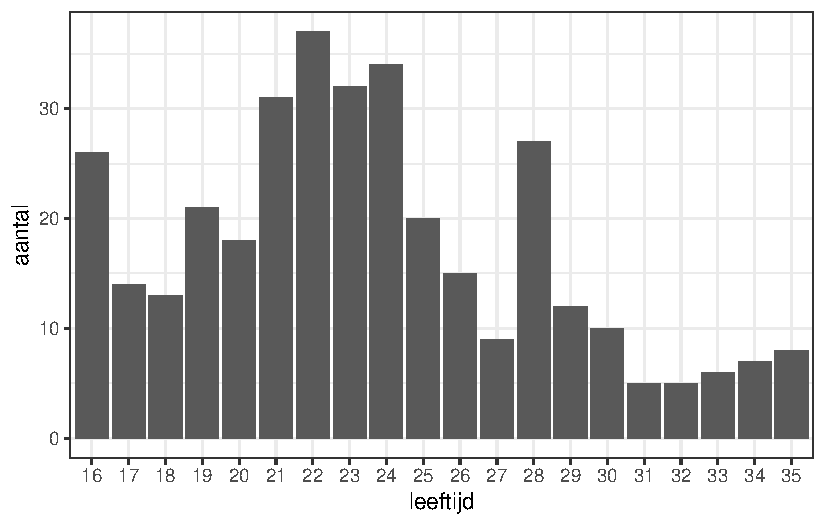
\includegraphics[keepaspectratio]{002-02-meetniveaus-visualisaties_files/figure-pdf/unnamed-chunk-8-1.pdf}}

De staafdiagram toont dat relatief veel respondenten tussen 21 en 24
jaar zijn, een leeftijd waarop jongeren veel uitgaan.

\subsection{Histogram}\label{sec-histogram}

Voor een lineaire variabele met juist relatief veel unieke waarden
gebruiken we meestal een histogram. Bij een een histogram worden
bepaalde waardes gegroepeerd tot één staaf, waardoor de presentatie
overzichtelijk blijft. Dit is hieronder weergeven voor de variabele
gemoed\_dinsdag\_na\_xtc\emph{.} Dit is een score tussen de 0 en 100 die
respondenten hebben gegeven hoe zich voelen op de dinsdag na xtc-gebruik
in het weekend, waarbij 0 voor negatief staat en 100 voor positief.

\begin{Shaded}
\begin{Highlighting}[]
\CommentTok{\# histogram van gemoedstoestand op dinsdag na XTC gebruik}
\FunctionTok{ggplot}\NormalTok{(data\_uitgaan, }\FunctionTok{aes}\NormalTok{(}\AttributeTok{x =}\NormalTok{ gemoed\_dinsdag\_na\_xtc)) }\SpecialCharTok{+}
  \FunctionTok{geom\_histogram}\NormalTok{(}\AttributeTok{bins =} \DecValTok{25}\NormalTok{, }\AttributeTok{fill =} \StringTok{"grey"}\NormalTok{, }\AttributeTok{colour =} \StringTok{"black"}\NormalTok{) }\SpecialCharTok{+}
  \FunctionTok{theme\_bw}\NormalTok{() }\SpecialCharTok{+} 
  \FunctionTok{ylab}\NormalTok{(}\StringTok{"aantal"}\NormalTok{) }\SpecialCharTok{+}
  \FunctionTok{xlab}\NormalTok{ (}\StringTok{"gemoedstoestand (negatief {-} positief)"}\NormalTok{) }\SpecialCharTok{+}
  \FunctionTok{xlim}\NormalTok{(}\DecValTok{0}\NormalTok{, }\DecValTok{100}\NormalTok{)}
\end{Highlighting}
\end{Shaded}

\pandocbounded{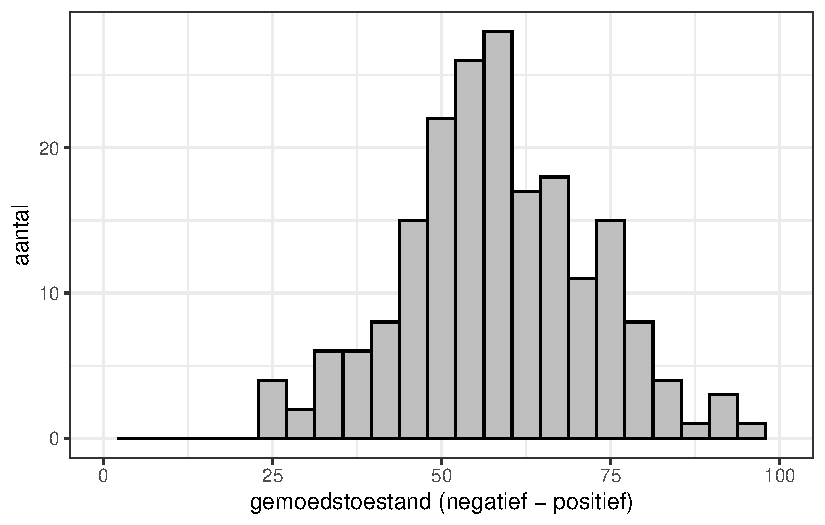
\includegraphics[keepaspectratio]{002-02-meetniveaus-visualisaties_files/figure-pdf/unnamed-chunk-9-1.pdf}}

\section{Meetniveau bepalen}\label{sec-meetniveaubepalen}

Het kan soms lastig zijn om het meetniveau te bepalen als je hier nog
weinig ervaring mee hebt. Het belangrijkste is altijd om goed te blijven
nadenken over de criteria die een meetniveau bepalen en hoe die van
toepassing zijn op een variabele. Daarbij kun je jezelf steeds vragen
stellen als:

\begin{itemize}
\tightlist
\item
  Bestaat deze variabele uit cijfers (numeriek/kwantitatief) of
  kwalitatieve categorieën?
\item
  Is er een rangorde of hiërarchie tussen de categorieën? En in hoeverre
  is er een gelijke afstand tussen de waarden (1-2-3 \ldots{} of, slecht
  - matig - goed)?
\item
  Heeft de variabele een absoluut nulpunt?
\end{itemize}

Belangrijk om te onthouden is dat veel variabelen geen inherent
meetniveau hebben. Het hangt af van de keuzes van de onderzoeker. Dat
wil zeggen dat \emph{hoe} ze worden gemeten leidend is voor welk
meetniveau een variabele heeft.

Leeftijd kun je bijvoorbeeld meten door respondenten hun leeftijd als
cijfer te laten invullen bij de vragenlijst (bijvoorbeeld 18, 24 of 33).
Dan krijg je een ratio variabele. Je kunt als antwoordopties in een
vragenlijst echter ook leeftijdscategorieën geven: 1) 16-20 jaar 2)
21-25 jaar 3) 26-30 jaar, etc. In dat geval meet je leeftijd als een
ordinale variabele, omdat de deze nu uit categorieën bestaat met een
rangorde waarvan de afstand tussen categorieën gelijk is.

Om het nog wat ingewikkelder te maken: je kunt variabelen ook aanpassen
in R waardoor het meetniveau verandert. Dit kan middels hercoderen, iets
waarmee je verder gaat oefenen in deze cursus.

Om dat met een kort voorbeeld te illustreren. Hieronder staan de eerste
zes observaties op de variabele leeftijd.

\begin{Shaded}
\begin{Highlighting}[]
\CommentTok{\# inspecteren eerste observaties leeftijd}
\FunctionTok{head}\NormalTok{(data\_uitgaan}\SpecialCharTok{$}\NormalTok{leeftijd)}
\end{Highlighting}
\end{Shaded}

\begin{verbatim}
[1] 22 23 18 28 19 18
\end{verbatim}

Je kunt zien dat de eerste respondent 22 jaar is, de tweede 23 jaar, de
derde 18 jaar, etc. Leeftijd is hier gemeten als kwantitatieve
variabele.

Nu hercoderen we deze leeftijden naar categorieën zoals hierboven
aangegeven.

\begin{Shaded}
\begin{Highlighting}[]
\CommentTok{\# hercoderen variabele leeftijd (van numeriek naar categorieën)}
\NormalTok{data\_uitgaan}\SpecialCharTok{$}\NormalTok{leeftijd\_cat }\OtherTok{\textless{}{-}} \FunctionTok{recode\_values}\NormalTok{(data\_uitgaan}\SpecialCharTok{$}\NormalTok{leeftijd,}
                                   \DecValTok{16}\SpecialCharTok{:}\DecValTok{20} \SpecialCharTok{\textasciitilde{}} \StringTok{"16{-}20 jaar"}\NormalTok{,}
                                   \DecValTok{21}\SpecialCharTok{:}\DecValTok{25} \SpecialCharTok{\textasciitilde{}} \StringTok{"21{-}25 jaar"}\NormalTok{,}
                                   \DecValTok{26}\SpecialCharTok{:}\DecValTok{30} \SpecialCharTok{\textasciitilde{}} \StringTok{"26{-}30 jaar"}\NormalTok{,}
                                   \DecValTok{31}\SpecialCharTok{:}\DecValTok{35} \SpecialCharTok{\textasciitilde{}} \StringTok{"31{-}35 jaar"}\NormalTok{)}
\CommentTok{\# nieuwe variabele leeftijd\_cat inspecteren}
\FunctionTok{head}\NormalTok{(data\_uitgaan}\SpecialCharTok{$}\NormalTok{leeftijd\_cat)}
\end{Highlighting}
\end{Shaded}

\begin{verbatim}
[1] "21-25 jaar" "21-25 jaar" "16-20 jaar" "26-30 jaar" "16-20 jaar"
[6] "16-20 jaar"
\end{verbatim}

Je ziet dat elke respondent nu in een categorie valt die hoort bij zijn
of haar leeftijd. De eerste respondent valt bijvoorbeeld in de categorie
`21-25 jaar' en de derde in categorie `16-20 jaar'. We hebben zojuist
van een ratio variabele een ordinale variabele gemaakt!

Let op dat de transformatie andersom niet mogelijk is: je kunt niet
zomaar van een ordinale variabele een kwantitatieve variabele maken. Van
respondenten in de categorie `16-20 jaar' weet je bijvoorbeeld niet hun
exacte leeftijd op basis van de informatie van deze variabele.

Ten slotte zul je onderzoek vaker \textbf{dichotome} (ook wel: binaire)
\textbf{variabelen} tegenkomen. Dit is een variabele die uitsluitend uit
twee antwoordmogelijkheden of waarden bestaat. Dit kunnen in principe
zowel nominale als ordinale variabelen zijn. Bijvoorbeeld:

\begin{itemize}
\tightlist
\item
  Nominaal: alcohol gedronken laatste jaar (ja/nee)
\item
  Ordinaal: leeftijd gemeten in twee categorieën (jonger dan 18 jaar/18
  jaar of ouder)
\end{itemize}

In sommige gevallen worden de antwoordcategorieën van dichotome
variabelen ook als 0/1 weergeven, waardoor het in principe numerieke
waarden worden maar kwalitatieve variabelen blijven. Dit is handig om
mee te rekenen, bijvoorbeeld als je het aandeel respondenten wil
berekenen dat alcohol heeft gedronken het laatste jaar (`0' voor nee en
`1' voor ja). Hier komen we in de practica op terug.

\section{Samenvatting}\label{samenvatting}

Het meetniveau gaat over het type variabele en wat voor soort informatie
deze bevat. Zoals we later zullen zien, is dit belangrijk om te weten
wat voor soort statistische toets we kunnen uitvoeren. We onderscheiden
de volgende meetniveaus (tussenhaakjes staat welke figuur we meestal
gebruiken):

\begin{itemize}
\tightlist
\item
  nominaal (staaf- of taartdiagram)
\item
  ordinaal (staafdiagram)
\item
  interval (staafdiagram of histogram)
\item
  ratio (staafdiagram of histogram)
\end{itemize}

\chapter{Centrum- en spreidingsmaten, normale verdeling en
z-score}\label{centrum--en-spreidingsmaten-normale-verdeling-en-z-score}

Inmiddels zijn we bekend met datasets, observaties, variabelen,
meetniveaus en figuren. We hebben ook benoemd dat statistiek draait om
het analyseren van \emph{variatie} met behulp van de variabelen die in
onze dataset zitten. Denk aan: variatie in drugsgebruik, uitgaansgedrag,
leeftijden en opleidingsniveau. Om de variatie te analyseren maken we
gebruik van diverse centrum- en spreidingsmaten. De meeste hiervan zul
je herkennen van eerdere wiskundelessen die je hebt gehad.

\section{Centrummaten}\label{centrummaten}

\subsection{Gemiddelde}\label{gemiddelde}

Het gemiddelde \(\bar{x}\) berekenen we simpelweg door voor de variabele
\(x\) alle observaties bij elkaar op te tellen \(\sum_{i=1}^n{x_i}\) en
dan te delen door het aantal observaties \(n\). Dit gaat middels de
volgende formule.

\[
\bar{x}=\frac{\sum_{i=1}^{n}{x_i}}{n}
\]

Formules berekenen en statistische toetsen uitvoeren kunnen we ook
handmatig in R doen. Dit is leerzaam, omdat het intuïtie creëert voor
hoe je statistisch onderzoek moet uitvoeren.

Stel we nemen vijf respondenten uit de dataset en bekijken hun leeftijd.
We vinden de volgende observaties voor leeftijd: 16, 22, 22, 28 en 33.

Hieronder berekenen we in R de gemiddelde leeftijd van deze vijf
respondenten.

\begin{Shaded}
\begin{Highlighting}[]
\CommentTok{\# handmatig gemiddelde berekenen}
\NormalTok{(}\DecValTok{16} \SpecialCharTok{+} \DecValTok{22} \SpecialCharTok{+} \DecValTok{22} \SpecialCharTok{+} \DecValTok{28} \SpecialCharTok{+} \DecValTok{33}\NormalTok{) }\SpecialCharTok{/} \DecValTok{5}
\end{Highlighting}
\end{Shaded}

\begin{verbatim}
[1] 24.2
\end{verbatim}

De gemiddelde leeftijd van deze vijf respondenten is is dus 24,2. In
plaats een handmatige berekening kun je het ook berekenen middels de
functie \emph{mean()} in R:

\begin{Shaded}
\begin{Highlighting}[]
\CommentTok{\# vector aanmaken}
\NormalTok{x }\OtherTok{\textless{}{-}} \FunctionTok{c}\NormalTok{(}\DecValTok{16}\NormalTok{, }\DecValTok{22}\NormalTok{, }\DecValTok{22}\NormalTok{, }\DecValTok{28}\NormalTok{, }\DecValTok{33}\NormalTok{)}
\FunctionTok{print}\NormalTok{(x)}
\end{Highlighting}
\end{Shaded}

\begin{verbatim}
[1] 16 22 22 28 33
\end{verbatim}

\begin{Shaded}
\begin{Highlighting}[]
\CommentTok{\# gemiddelde berekenen}
\FunctionTok{mean}\NormalTok{(x)}
\end{Highlighting}
\end{Shaded}

\begin{verbatim}
[1] 24.2
\end{verbatim}

Eerst hebben we een vector, of eigenlijk een variabele, aangemaakt met
de vijf observaties. Via de functie \emph{mean()} bereken je vervolgens
het gemiddelde.

\subsection{Mediaan}\label{mediaan}

De mediaan is het getal waar het midden van het aantal observaties is
bereikt (50\%), oftewel de middelste observatie.

Bij de leeftijdsreeks (16, 22, \ul{22}, 28, 33) is dit 22 jaar.

Bij een even aantal cijfers zoals (16, 22, 22, 25, 28, 33) neem je het
midden van de middelste twee getallen. In dit geval is dat 23,5 (tussen
22 en 25 jaar).

In R bereken je de mediaan via de functie \emph{median().}

\begin{Shaded}
\begin{Highlighting}[]
\CommentTok{\# oneven aantal observaties}
\FunctionTok{median}\NormalTok{(x)}
\end{Highlighting}
\end{Shaded}

\begin{verbatim}
[1] 22
\end{verbatim}

\begin{Shaded}
\begin{Highlighting}[]
\CommentTok{\# even aantal observaties}
\NormalTok{y }\OtherTok{\textless{}{-}} \FunctionTok{c}\NormalTok{(}\DecValTok{16}\NormalTok{, }\DecValTok{22}\NormalTok{, }\DecValTok{22}\NormalTok{, }\DecValTok{25}\NormalTok{, }\DecValTok{28}\NormalTok{, }\DecValTok{33}\NormalTok{)}
\FunctionTok{print}\NormalTok{(y)}
\end{Highlighting}
\end{Shaded}

\begin{verbatim}
[1] 16 22 22 25 28 33
\end{verbatim}

\begin{Shaded}
\begin{Highlighting}[]
\FunctionTok{median}\NormalTok{(y)}
\end{Highlighting}
\end{Shaded}

\begin{verbatim}
[1] 23.5
\end{verbatim}

\subsection{Modus}\label{modus}

De modus is de waarde die het vaakst voorkomt in een variabele.

Bij de leeftijdsreeks (16, \ul{22}, \ul{22}, 28, 33) is dit 22 jaar
omdat deze leeftijd tweemaal voorkomt en de rest slechts één keer.

In R bereken je de modus via de functie \emph{mfv().}

\begin{Shaded}
\begin{Highlighting}[]
\CommentTok{\# modus berekenen}
\FunctionTok{mfv}\NormalTok{(x)}
\end{Highlighting}
\end{Shaded}

\begin{verbatim}
[1] 22
\end{verbatim}

\section{Spreidingsmaten}\label{spreidingsmaten}

Tekst toevoegen over belang spreiding =\textgreater{} Joost

\subsection{Bereik, minimum en maximum}\label{bereik-minimum-en-maximum}

Het bereik \(R\) van een variabele is de afstand tussen de laagste
(minimum: \(x_{min}\)) en hoogste (maximum: \(x_{max}\)) waarde. Dit
bereken je eenvoudig door de hoogste waarde minus de laagste waarde te
nemen:

\[R=x_{max}-x_{min}\]

Bij de leeftijdsreeks (16, 22, 22, 28, 33) is het minimum 16 en het
maximum 33. Het bereik is dus \(R=x_{max}-x_{min}=33-16=17\)

\begin{Shaded}
\begin{Highlighting}[]
\CommentTok{\# handmatig bereik berekenen}
\DecValTok{33} \SpecialCharTok{{-}} \DecValTok{16}
\end{Highlighting}
\end{Shaded}

\begin{verbatim}
[1] 17
\end{verbatim}

Je kunt in R het minimum en maximum opvragen met de functies
\emph{min()} en \emph{max()}. Ook kun je allebei tegelijk krijgen met de
functie \emph{range()}

\begin{Shaded}
\begin{Highlighting}[]
\CommentTok{\# minimum opvragen}
\FunctionTok{min}\NormalTok{(x)}
\end{Highlighting}
\end{Shaded}

\begin{verbatim}
[1] 16
\end{verbatim}

\begin{Shaded}
\begin{Highlighting}[]
\CommentTok{\# maximum opvragen}
\FunctionTok{max}\NormalTok{(x)}
\end{Highlighting}
\end{Shaded}

\begin{verbatim}
[1] 33
\end{verbatim}

\begin{Shaded}
\begin{Highlighting}[]
\CommentTok{\# minimum en maximum opvragen}
\FunctionTok{range}\NormalTok{(x)}
\end{Highlighting}
\end{Shaded}

\begin{verbatim}
[1] 16 33
\end{verbatim}

De functie \emph{range()} geeft je alleen het minimum en maximum. Als je
het bereik wilt weten, moet je zelf het minimum van het maximum
aftrekken:

\begin{Shaded}
\begin{Highlighting}[]
\CommentTok{\# bereik berekenen}
\FunctionTok{max}\NormalTok{(x) }\SpecialCharTok{{-}} \FunctionTok{min}\NormalTok{(x)}
\end{Highlighting}
\end{Shaded}

\begin{verbatim}
[1] 17
\end{verbatim}

\subsection{Variantie}\label{variantie}

De variantie is een maat voor de spreiding van een variabele die
aangeeft hoeveel de waardes onderling van elkaar verschillen. In de
statistiek van de sociale wetenschappen zijn er twee soorten variantie:
de populatievariantie en steekproefvariantie. Hier komen we later op
terug, we rekenen nu voorlopig verder met de steekproefvariantie. De
formule daarvoor is:

\[
S^2=\frac{\sum_{i=1}^{n}{(x_i-\bar{x})^2}}{n-1}
\] De steekproefvariantie \(S^2\) kun je bereken in een aantal stappen.

Dit doen we aan de hand van de leeftijdsreeks (16, 22, 22, 28, 33) en
het gemiddelde hiervan \(\bar{x}\) = 24,2

Eerst berekenen we voor elke observatie de afstand tot het gemiddelde
(de deviatie):

{\def\LTcaptype{none} % do not increment counter
\begin{longtable}[]{@{}cc@{}}
\toprule\noalign{}
\(x_i\) & \(x_i-\bar{x}\) \\
\midrule\noalign{}
\endhead
\bottomrule\noalign{}
\endlastfoot
16 & 16 - 24,2 = -8,2 \\
22 & 22 - 24,2 = -2,2 \\
22 & 22 - 24,2 = -2,2 \\
28 & 28 - 24,2 = 3,8 \\
33 & 33 - 24,2 = 8,8 \\
\end{longtable}
}

De optelsom van alle deviaties moet altijd nul zijn: -8,2 + -2,2 + -2,2
+ 3,8 + 8,8 = 0

In de volgende stap kwadrateren we alle deviaties:

{\def\LTcaptype{none} % do not increment counter
\begin{longtable}[]{@{}ccc@{}}
\toprule\noalign{}
\(x_i\) & \(x_i-\bar{x}\) & \((x_i-\bar{x})^2\) \\
\midrule\noalign{}
\endhead
\bottomrule\noalign{}
\endlastfoot
16 & 16 - 24,2 = -8,2 & \((-8,2)^2 = 67,24\) \\
22 & 22 - 24,2 = -2,2 & \((-2,2)^2 = 4,84\) \\
22 & 22 - 24,2 = -2,2 & \((-2,2)^2 = 4,84\) \\
28 & 28 - 24,2 = 3,8 & \(3,8^2 = 14,44\) \\
33 & 33 - 24,2 = 8,8 & \(8,8^2 = 77,44\) \\
\end{longtable}
}

Daarvan nemen we de som der kwadraten
\(\sum_{i=1}^{n}{(x_i-\bar{x})^2}\) : 67,24 + 4,84 + 4,84 + 14,44 +
77,44 = 168,8

In de laatste stap delen we de som der kwadraten door het aantal
observaties minus één (\(n-1\)) :

168,8 / (5-1) = 42,2

De steekproefvariantie van de leeftijd van vijf respondenten is dus
42,2.

Deze stappen kunnen we ook in R uitvoeren.

\begin{Shaded}
\begin{Highlighting}[]
\CommentTok{\# deviatie voor elke leeftijd}
\NormalTok{x\_deviatie }\OtherTok{\textless{}{-}}\NormalTok{ x }\SpecialCharTok{{-}} \FunctionTok{mean}\NormalTok{(x) }\CommentTok{\# voor elke waarde van x minus het gemiddelde}
\FunctionTok{print}\NormalTok{(x\_deviatie)}
\end{Highlighting}
\end{Shaded}

\begin{verbatim}
[1] -8.2 -2.2 -2.2  3.8  8.8
\end{verbatim}

\begin{Shaded}
\begin{Highlighting}[]
\CommentTok{\# kwadrateren van deviaties}
\NormalTok{x\_deviatie\_kwa }\OtherTok{\textless{}{-}}\NormalTok{ x\_deviatie}\SpecialCharTok{\^{}}\DecValTok{2} \CommentTok{\# voor elke deviatie het kwadraat nemen}
\FunctionTok{print}\NormalTok{(x\_deviatie\_kwa)}
\end{Highlighting}
\end{Shaded}

\begin{verbatim}
[1] 67.24  4.84  4.84 14.44 77.44
\end{verbatim}

\begin{Shaded}
\begin{Highlighting}[]
\CommentTok{\# som der kwadraten}
\FunctionTok{sum}\NormalTok{(x\_deviatie\_kwa) }\CommentTok{\# sum() neemt de som van een vector}
\end{Highlighting}
\end{Shaded}

\begin{verbatim}
[1] 168.8
\end{verbatim}

\begin{Shaded}
\begin{Highlighting}[]
\CommentTok{\# steekproefvariantie berekenen}
\NormalTok{variantie\_stkpr }\OtherTok{\textless{}{-}} \FunctionTok{sum}\NormalTok{(x\_deviatie\_kwa) }\SpecialCharTok{/}\NormalTok{ (}\FunctionTok{length}\NormalTok{(x) }\SpecialCharTok{{-}} \DecValTok{1}\NormalTok{) }\CommentTok{\# length() berekent het aantal rijen}
\FunctionTok{print}\NormalTok{(variantie\_stkpr)}
\end{Highlighting}
\end{Shaded}

\begin{verbatim}
[1] 42.2
\end{verbatim}

In R kun je met de functie \emph{var()} de steekproefvariantie ook
direct berekenen

\begin{Shaded}
\begin{Highlighting}[]
\CommentTok{\# steekproefvariantie }
\FunctionTok{var}\NormalTok{(x)}
\end{Highlighting}
\end{Shaded}

\begin{verbatim}
[1] 42.2
\end{verbatim}

\subsection{Standaarddeviatie}\label{standaarddeviatie}

De variantie is een handig getal om mee te rekenen, maar heeft meestal
op zichzelf niet zoveel betekenis. Daarom wordt in onderzoek gebruik
gemaakt van de standaarddeviatie (ook wel standaardafwijking genoemd).
In combinatie met het gemiddelde en het bereik, geeft de
standaarddeviatie meestal een redelijke indicatie van de spreiding van
een lineaire variabele (hier komen we later weer op terug). Hoewel
wiskundig niet helemaal correct, wordt de standaarddeviatie ook wel
gezien als `de gemiddelde afstand tot het gemiddelde'.

De standaarddeviatie is de wortel van de steekproefvariantie:

\[
s=\sqrt\frac{\sum_{i=1}^{n}{(x_i-\bar{x})^2}}{n-1}
\]

De standaarddeviatie van ons voorbeeld met de leeftijd van vijf
respondenten is:

\(s=\sqrt{42,2}=6,50\)

Je zou dus kunnen zeggen dat een willekeurige persoon van de vijf
respondenten `gemiddeld' 6,5 jaar afwijkt van de gemiddelde leeftijd van
24,2 jaar.

\begin{Shaded}
\begin{Highlighting}[]
\CommentTok{\# standaarddeviatie berekenen}
\FunctionTok{sqrt}\NormalTok{(variantie\_stkpr) }\CommentTok{\# sqrt() berekent de wortel over een getal/vector}
\end{Highlighting}
\end{Shaded}

\begin{verbatim}
[1] 6.496153
\end{verbatim}

Je kunt de standaarddeviatie ook direct in R krijgen met \emph{sd()}

\begin{Shaded}
\begin{Highlighting}[]
\CommentTok{\# standaarddeviatie}
\FunctionTok{sd}\NormalTok{(x)}
\end{Highlighting}
\end{Shaded}

\begin{verbatim}
[1] 6.496153
\end{verbatim}

\section{Toepassing op de dataset}\label{toepassing-op-de-dataset}

We hebben hierboven middels een eenvoudig voorbeeld laten zien hoe de
centrum- en spreidingsmaten berekend worden. In onderzoek willen we deze
informatie voor variabelen in de hele dataset weten, zodat we snel
kunnen zien hoe onze data in elkaar zit.

We vragen hier het gemiddelde, de mediaan en de modus op voor leeftijd
in de complete dataset.

\begin{Shaded}
\begin{Highlighting}[]
\CommentTok{\# centrummaten opvragen}
\FunctionTok{mean}\NormalTok{(data\_uitgaan}\SpecialCharTok{$}\NormalTok{leeftijd) }\CommentTok{\# gemiddelde}
\end{Highlighting}
\end{Shaded}

\begin{verbatim}
[1] 23.52
\end{verbatim}

\begin{Shaded}
\begin{Highlighting}[]
\FunctionTok{median}\NormalTok{(data\_uitgaan}\SpecialCharTok{$}\NormalTok{leeftijd) }\CommentTok{\# mediaan}
\end{Highlighting}
\end{Shaded}

\begin{verbatim}
[1] 23
\end{verbatim}

\begin{Shaded}
\begin{Highlighting}[]
\FunctionTok{mfv}\NormalTok{(data\_uitgaan}\SpecialCharTok{$}\NormalTok{leeftijd) }\CommentTok{\# modus}
\end{Highlighting}
\end{Shaded}

\begin{verbatim}
[1] 22
\end{verbatim}

De gemiddelde leeftijd is 23,5 jaar, de mediaan is 23 jaar en de modus
is 22 jaar. Deze waarden liggen dus dicht bij elkaar.

We kunnen ook het minimum, maximum, bereik en de standaarddeviatie
berekenen.

\begin{Shaded}
\begin{Highlighting}[]
\CommentTok{\# spreidingsmaten opvragen}
\FunctionTok{range}\NormalTok{(data\_uitgaan}\SpecialCharTok{$}\NormalTok{leeftijd) }\CommentTok{\# minimum en maximum}
\end{Highlighting}
\end{Shaded}

\begin{verbatim}
[1] 16 35
\end{verbatim}

\begin{Shaded}
\begin{Highlighting}[]
\FunctionTok{max}\NormalTok{(data\_uitgaan}\SpecialCharTok{$}\NormalTok{leeftijd) }\SpecialCharTok{{-}} \FunctionTok{min}\NormalTok{(data\_uitgaan}\SpecialCharTok{$}\NormalTok{leeftijd) }\CommentTok{\# bereik}
\end{Highlighting}
\end{Shaded}

\begin{verbatim}
[1] 19
\end{verbatim}

\begin{Shaded}
\begin{Highlighting}[]
\FunctionTok{sd}\NormalTok{(data\_uitgaan}\SpecialCharTok{$}\NormalTok{leeftijd) }\CommentTok{\#standaarddeviatie}
\end{Highlighting}
\end{Shaded}

\begin{verbatim}
[1] 4.782178
\end{verbatim}

De minimumleeftijd is 16 jaar, de maximumleeftijd is 35 jaar en het
leeftijdsbereik is 19 jaar. De standaarddeviatie is 4,8 jaar.

Veel van deze statistieken (min., max., mediaan, gemiddelde) kun je ook
in één keer bekijken middels de functie \emph{summary()}

\begin{Shaded}
\begin{Highlighting}[]
\CommentTok{\# meerdere statistieken tegelijkertijd opvragen}
\FunctionTok{summary}\NormalTok{(data\_uitgaan}\SpecialCharTok{$}\NormalTok{leeftijd)}
\end{Highlighting}
\end{Shaded}

\begin{verbatim}
   Min. 1st Qu.  Median    Mean 3rd Qu.    Max. 
  16.00   20.00   23.00   23.52   27.00   35.00 
\end{verbatim}

Je ziet dat de \emph{summary()} functie ook de waardes voor 1st Qu. en
3rd Qu. geeft. Dit zijn het eerste en derde kwartiel, de grenzen waarbij
respectievelijk 25\% (Q1) en 75\% (Q3) van de data ligt. In dit geval
dus 20,0 en 27,0 jaar. Het tweede kwartiel (Q2) is de mediaan, dit is op
de grens van 50\% van de data.

\subsection{Doosdiagram}\label{doosdiagram}

Er bestaat ook een manier om de spreiding van een lineaire variabele te
visualiseren. Dit is via een \textbf{doosdiagram}.

\begin{Shaded}
\begin{Highlighting}[]
\CommentTok{\# doosdiagram maken}
\FunctionTok{ggplot}\NormalTok{(data\_uitgaan, }\FunctionTok{aes}\NormalTok{(}\AttributeTok{x =}\NormalTok{ leeftijd)) }\SpecialCharTok{+} 
  \FunctionTok{geom\_boxplot}\NormalTok{() }\CommentTok{\# doosdiagram}
\end{Highlighting}
\end{Shaded}

\pandocbounded{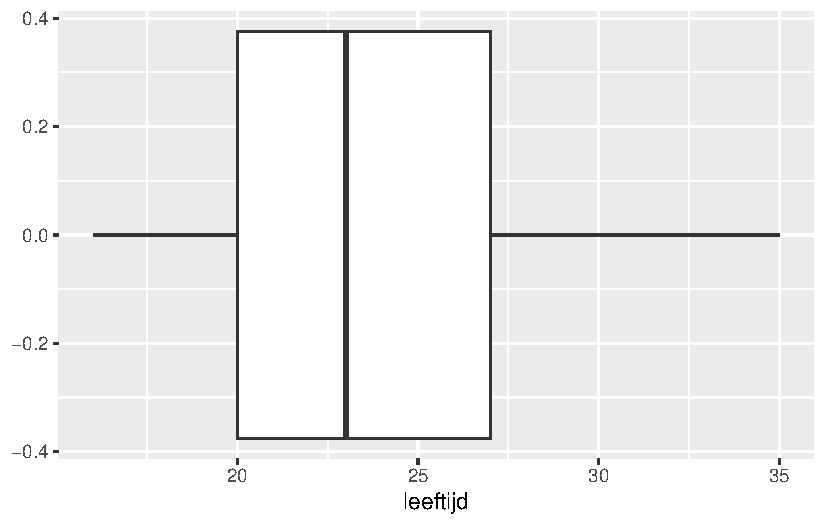
\includegraphics[keepaspectratio]{002-03-centrum-en-spreidingsmaten_files/figure-pdf/unnamed-chunk-16-1.pdf}}

Zoals we inmiddels hebben gezien, kan de presentatie van de figuur kan
nog verbeterd worden.

\begin{Shaded}
\begin{Highlighting}[]
\CommentTok{\# doosdiagram maken}
\FunctionTok{ggplot}\NormalTok{(data\_uitgaan, }\FunctionTok{aes}\NormalTok{(}\AttributeTok{x =}\NormalTok{ leeftijd)) }\SpecialCharTok{+} 
  \FunctionTok{geom\_boxplot}\NormalTok{() }\SpecialCharTok{+} \CommentTok{\# doosdiagram}
  \FunctionTok{theme\_bw}\NormalTok{() }\SpecialCharTok{+}
  \FunctionTok{scale\_x\_continuous}\NormalTok{(}\AttributeTok{breaks =} \FunctionTok{seq}\NormalTok{(}\DecValTok{16}\NormalTok{, }\DecValTok{35}\NormalTok{, }\AttributeTok{by =} \DecValTok{1}\NormalTok{)) }\SpecialCharTok{+} \CommentTok{\# aanpassen labels x{-}as, van 16 tot 35 met steeds 1 eenheid ertussen (1 jaar)}
  \FunctionTok{scale\_y\_continuous}\NormalTok{(}\AttributeTok{breaks =} \ConstantTok{NULL}\NormalTok{) }\CommentTok{\# verwijderen labels y{-}as (hebben geen betekenis hier)}
\end{Highlighting}
\end{Shaded}

\pandocbounded{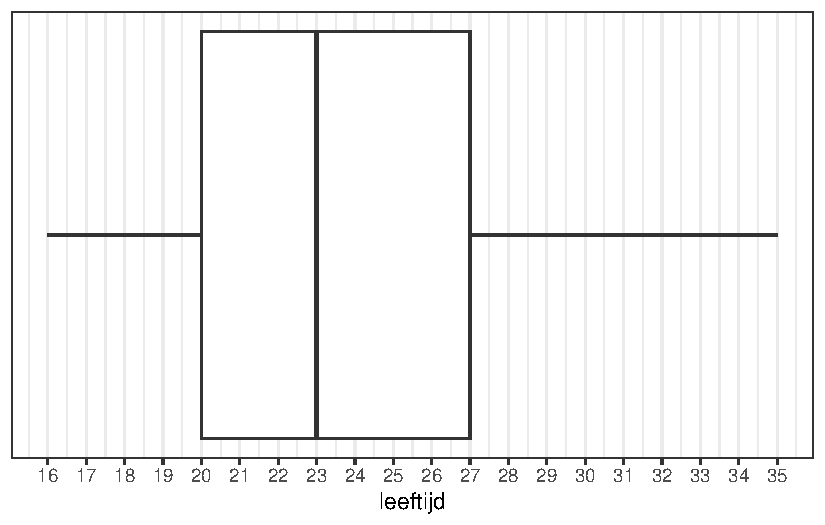
\includegraphics[keepaspectratio]{002-03-centrum-en-spreidingsmaten_files/figure-pdf/unnamed-chunk-17-1.pdf}}

Een doosdiagram weergeeft de spreiding van een variabele en bevat het
minimum en maximum, en de grenzen van het 1ste kwartiel (Q1), mediaan
(Q2) en 3de kwartiel (Q3). De afstand tussen het 1ste en 3de kwartiel
wordt ook wel de \textbf{interkwartielafstand} genoemd.

Je kunt aan bovenstaande figuur bijvoorbeeld zien dat alle waarden
tussen het 1ste kwartiel en mediaan tussen de 20 en 23 jaar liggen. Het
hoogste kwartiel (Q4) omvat relatief veel leeftijden, van 27 tot 35
jaar.

Vergelijk deze doosdiagram met de staafdiagram van leeftijd
(\hyperref[sec-intervalratioux5cux257D]{Staafdigram leeftijd}). Je ziet
dat er verschillende manieren zijn om data te visualiseren.

\section{Normale verdeling}\label{sec-normaleverdeling}

We hebben diverse centrum- en spreidingsmaten besproken. Deze kunnen we
gebruiken om de verdeling van een variabele te visualiseren, afhankelijk
van het meetniveau van de variabele (zie ook
\hyperref[meetniveaus-en-visualisaties]{Meetniveaus en visualisaties}).
Een van de meest bekende verdelingen in de statistiek is de
\textbf{normale verdeling} (of normaalverdeling). Deze wordt gebruikt om
verdeling van kwantitatieve variabelen te beschrijven, denk bijvoorbeeld
aan lengte of IQ.

De normale verdeling heeft een aantal kenmerken:

\begin{itemize}
\tightlist
\item
  De verdeling bestaat uit een gemiddelde \(\bar{x}\) en
  standaarddeviatie \(s\)
\item
  Het gemiddelde en de mediaan zijn in principe gelijk aan elkaar. Dit
  betekent dat de verdeling symmetrisch is (50\% van de observaties
  bevindt zich links van het gemiddelde, en 50\% rechts)
\end{itemize}

Hieronder staat een afbeelding van de normale verdeling.
\pandocbounded{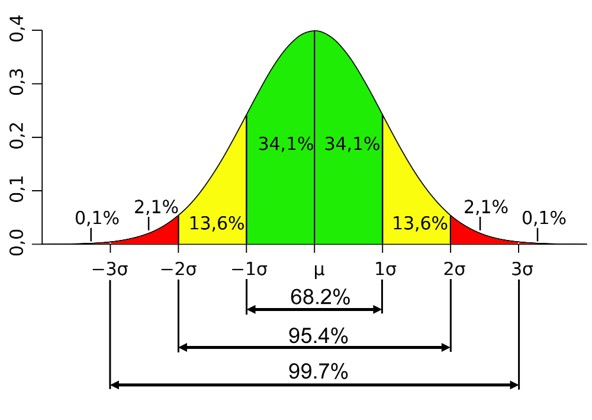
\includegraphics[keepaspectratio,alt={Normale verdeling}]{afbeeldingen/Normale_verdeling.jpg}}

De notatie in deze afbeelding is iets anders dan je tot nu toe gewend
bent. Het gemiddelde wordt aangegeven met \(\mu\) (spreek je uit als:
mu) en de standaardafwijking met \(\sigma\) (spreek je uit als: sigma).
Deze symbolen zijn eigenlijk hetzelfde als \(\bar{x}\) en \(s\) , alleen
gebruiken we \(\mu\) en \(\sigma\) om eigenschappen van de populatie te
beschrijven terwijl \(\bar{x}\) en \(s\) gelden voor de steekproef (zie
ook \href{formuleblad.qmd}{Formuleblad}). Dit verschil komt terug bij
\href{003-01-steekproeven.qmd}{Inferentiële statistiek}. Voor nu kun je
er even van uitgaan dat ze hetzelfde betekenen.

De normaalverdeling noemen we ook wel een \emph{kans}verdeling, omdat
(onder bepaalde assumpties) een bepaald oppervlak onder de grafiek
correspondeert met de kans op een waarde of uitkomst. Zo kun in de
afbeelding bijvoorbeeld zien dat tussen één standaarddeviatie onder het
gemiddelde (\(-1\sigma\)) en één standaarddeviatie boven het gemiddelde
(\(1\sigma\)) 68,2\% van alle waarden liggen. Verder geldt:

\begin{itemize}
\item
  tussen \(-2\sigma\) en \(2\sigma\) liggen 95,4\% van alle observaties
\item
  tussen \(-3\sigma\) en \(3\sigma\) liggen 99,7\% van alle observaties
\end{itemize}

Dat een bepaald bereik op basis van standaarddeviaties correspondeert
met een zeker percentage van alle observaties, staat ook wel bekend als
\textbf{de empirische regel.} Je zult later bij het berekenen van een
betrouwbaarheidsinterval en hypothese toetsen gaan zien waarom dit
relevant is.

Het is belangrijk om op te merken dat in de praktijk variabelen zelden
exact normaal verdeeld zijn, ze volgen dus niet precies de verdeling
zoals hierboven weergeven. Zo kunnen kwantitatieve variabelen ook
linksscheef of rechtsscheef verdeeld zijn, die daarvoor deze
\href{https://www.scribbr.nl/statistiek/skewness-scheefheid/}{link}.

\section{Z-score}\label{sec-zscore}

Om inzicht te krijgen in de relatieve positie van een bepaalde
observatie ten opzichte van het gemiddelde, kunnen we ten slotte een
z-score berekenen. Een z-score is een gestandaardiseerde maat die
aangeeft hoeveel standaarddeviaties een waarde van het gemiddelde ligt.
Daarbij geldt dat, door het standaardiseren, het gemiddelde altijd 0 is
en de standaardafwijking 1. De z-score heeft de volgende formule:

\[ z=\frac{x-\bar{x}}{s} \]

De berekening is vrij eenvoudig: je trekt het gemiddelde \(\bar{x}\) af
van de specifieke waarde \(x\) en deelt dit door de standaardafwijking
\(s\) van de originele variabele.

Laten we dit illustreren aan de hand van een voorbeeld. Bij
\hyperref[sec-histogram]{Histogram} zag je de variabele
gemoed\_dinsdag\_na\_xtc\emph{,} die staat voor een score tussen de 0 en
100 over hoe positief respondenten zich voelen op de dinsdag na
xtc-gebruik in het weekend. We vragen eerst het gemiddelde en de
standaarddeviatie op.

\begin{Shaded}
\begin{Highlighting}[]
\CommentTok{\# gemiddelde en standaarddeviatie (met verwijderen missende waarden via na.rm)}
\FunctionTok{mean}\NormalTok{(data\_uitgaan}\SpecialCharTok{$}\NormalTok{gemoed\_dinsdag\_na\_xtc, }\AttributeTok{na.rm =} \ConstantTok{TRUE}\NormalTok{)}
\end{Highlighting}
\end{Shaded}

\begin{verbatim}
[1] 58.27179
\end{verbatim}

\begin{Shaded}
\begin{Highlighting}[]
\FunctionTok{sd}\NormalTok{(data\_uitgaan}\SpecialCharTok{$}\NormalTok{gemoed\_dinsdag\_na\_xtc, }\AttributeTok{na.rm =} \ConstantTok{TRUE}\NormalTok{)}
\end{Highlighting}
\end{Shaded}

\begin{verbatim}
[1] 14.03798
\end{verbatim}

We nemen als voorbeeld iemand die score 30 heeft ingevuld. Dan weten we
in principe alle relevante informatie en kunnen we dit invullen in de
formule:

\[ z=\frac{x-\bar{x}}{s}=\frac{30-58,3}{14,0} \]

We kunnen R gebruiken om dit uit te rekenen:

\begin{Shaded}
\begin{Highlighting}[]
\NormalTok{(}\DecValTok{30}\FloatTok{{-}58.3}\NormalTok{)}\SpecialCharTok{/}\FloatTok{14.0}
\end{Highlighting}
\end{Shaded}

\begin{verbatim}
[1] -2.021429
\end{verbatim}

De persoon met score 30 bevindt dus ongeveer 2 standaarddeviaties onder
het gemiddelde. Zoals de normale verdeling laat zien, is dit een vrij
extreme score (slechts 2,2\% van de waardes ligt nog onder 2
standaarddeviaties).\footnote{Vergelijk dit ook visueel met de verdeling
  van gemoed\_dinsdag\_na\_xtc bij \hyperref[sec-histogram]{Histogram}.
  Waar ligt score 30 t.o.v. de rest van de verdeling?} Deze partyprins
of -prinses voelt zich dus niet zo lekker vergeleken met de rest op de
dinsdag na een wild weekend!

\chapter{Relaties tussen variabelen}\label{relaties-tussen-variabelen}

We hebben tot nu toe gekeken naar wat voor verschillende variabelen er
zijn (meetniveaus), hoe we de onderliggende data kunnen visualiseren, en
met welke statistische maten we deze variabelen kunnen beschrijven. In
onderzoek zijn we niet alleen geïnteresseerd in variabelen zelf, maar
nog meer in de \textbf{relaties} daartussen. Voor onze dataset zouden we
bijvoorbeeld de volgende vragen kunnen stellen:

\begin{itemize}
\tightlist
\item
  Wat is het verschil tussen mannen en vrouwen in drugsgebruik?
\item
  In hoeverre denken gebruikers anders over de acceptatie van drugs dan
  niet-gebruikers?
\item
  Wat is de relatie tussen verschillende soorten drugsgebruik?
\end{itemize}

Om dergelijke vragen te beantwoorden, moeten we data van verschillende
variabelen met elkaar combineren. Daarbij moeten we ons steeds afvragen
hoe we deze relaties inzichtelijk willen maken. Het is goed om te
realiseren dat hier niet altijd één juist antwoord voor is. Er zijn
meerdere manieren om data en relaties te presenteren, waarbij de
creativiteit van de onderzoeker ertoe doet. Over het algemeen zijn er
wel gebaande paden die we kunnen volgen.

We letten bij het onderzoeken van relaties tussen variabelen vooral op
hun meetniveau. Hebben we bijvoorbeeld te maken met twee kwalitatieve
variabelen, één kwalitatief en één kwantitatief, of twee kwantitatieve
variabelen? Daaruit kunnen we vaak afleiden wat de handigste manier is
om een relatie te presenteren. Denk dus altijd eerst goed na wat het
meetniveau van een variabele is.

\section{Kwalitatief vs.~kwalitatief}\label{kwalitatief-vs.-kwalitatief}

\subsection{Nominaal vs.~nominaal}\label{nominaal-vs.-nominaal}

Als we de relatie tussen twee nominale variabelen willen presenteren,
kunnen we een eenvoudige kruistabel maken in R. We kijken in dit
voorbeeld naar de relatie tussen geslacht (man/vrouw/anders) en of men
heeft gevapet in het afgelopen jaar (ja/nee). We gaan er hier vanuit dat
er geen rangorde bestaat tussen wel of niet vapen en het dus een
nominale variabele betreft.

In hoofdstuk xxx hebben we al een tabel gemaakt voor geslacht. We kunnen
aan het commando \emph{table()} een variabele (vapen\_laatste\_jaar)
toevoegen om een kruistabel te krijgen.

\begin{Shaded}
\begin{Highlighting}[]
\CommentTok{\# kruistabel tussen geslacht en vapen laatste jaar}
\FunctionTok{table}\NormalTok{(data\_uitgaan}\SpecialCharTok{$}\NormalTok{vapen\_laatste\_jaar, data\_uitgaan}\SpecialCharTok{$}\NormalTok{geslacht) }\CommentTok{\# vapen in de rijen, }
\end{Highlighting}
\end{Shaded}

\begin{verbatim}
     
      man vrouw anders
  nee  85    73      0
  ja   93    97      2
\end{verbatim}

\begin{Shaded}
\begin{Highlighting}[]
                                              \CommentTok{\# geslacht in de kolommen}
\end{Highlighting}
\end{Shaded}

We zien in bovenstaande tabel hoe vaak personen van een bepaald geslacht
hebben gevapet het afgelopen jaar. Zo kun je zien dat 73 vrouwen niet
hebben gevapet en 97 wel.

Visueel krijgen we vaak een beter inzicht in de verdeling van variabelen
en de relaties daartussen. We kunnen de verdeling voor
vapen\_laatste\_jaar uitgesplitst naar geslacht daarom apart weergeven
in een figuur. De meest gangbare manier om de relatie tussen twee
variabelen visueel te weergeven is een staafdiagram. We laten voor
eenvoud de categorie `anders' even buiten beschouwing hier.

\begin{Shaded}
\begin{Highlighting}[]
\CommentTok{\# samenvatten van de relevante data}
\NormalTok{geslacht\_vapen }\OtherTok{\textless{}{-}}\NormalTok{ data\_uitgaan }\SpecialCharTok{|\textgreater{}}
  \FunctionTok{filter}\NormalTok{(geslacht }\SpecialCharTok{!=} \StringTok{"anders"}\NormalTok{) }\SpecialCharTok{|\textgreater{}} \CommentTok{\# categorie \textquotesingle{}anders\textquotesingle{} eruit laten }
  \FunctionTok{group\_by}\NormalTok{(geslacht, vapen\_laatste\_jaar) }\SpecialCharTok{|\textgreater{}} \CommentTok{\# groeperen op variabelen}
  \FunctionTok{summarise}\NormalTok{(}\AttributeTok{n =} \FunctionTok{n}\NormalTok{()) }\CommentTok{\# aantal respondenten per categorie berekenen}

\CommentTok{\# staafdiagram maken voor relatie geslacht en vapen }
\FunctionTok{ggplot}\NormalTok{(geslacht\_vapen, }\FunctionTok{aes}\NormalTok{(}\AttributeTok{x =}\NormalTok{ geslacht, }\AttributeTok{y =}\NormalTok{ n, }\AttributeTok{fill =}\NormalTok{ vapen\_laatste\_jaar)) }\SpecialCharTok{+}
  \FunctionTok{geom\_col}\NormalTok{(}\AttributeTok{position =} \StringTok{"dodge"}\NormalTok{) }\SpecialCharTok{+}
  \FunctionTok{theme\_bw}\NormalTok{() }\SpecialCharTok{+}
  \FunctionTok{ylab}\NormalTok{(}\StringTok{"aantal"}\NormalTok{) }\SpecialCharTok{+}
  \FunctionTok{labs}\NormalTok{(}\AttributeTok{fill =} \StringTok{"Vapen laatste jaar"}\NormalTok{)}
\end{Highlighting}
\end{Shaded}

\pandocbounded{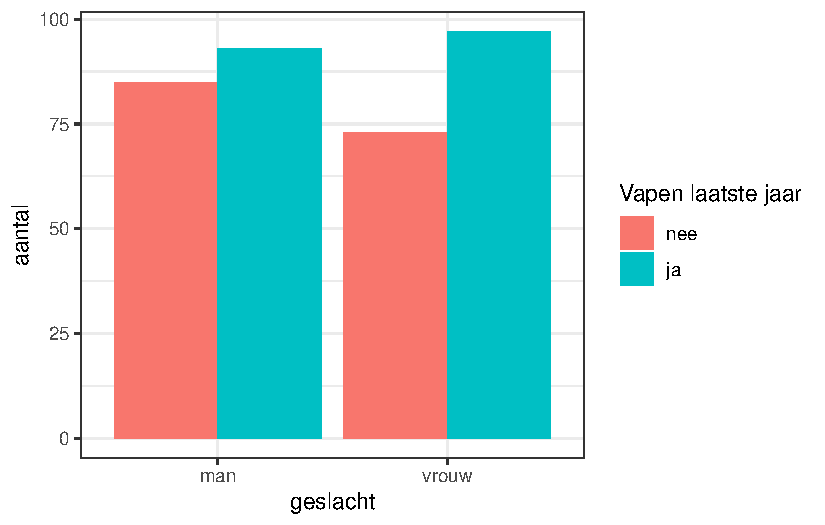
\includegraphics[keepaspectratio]{002-04-relatiesvariabelen_files/figure-pdf/unnamed-chunk-3-1.pdf}}

We zien nu in een oogoopslag wat de verschillen zijn in aantallen tussen
mannen en vrouwen die vapeten het laatste jaar.

De absolute aantallen geven slechts gedeeltelijk inzicht in wat
verhoudingen zijn binnen de relatie tussen geslacht en vapen. Daarom is
het handig ook de kolompercentages te bereken. Dit doen we door
\emph{prop.table()} toe te voegen aan de kruistabel.

\begin{Shaded}
\begin{Highlighting}[]
\CommentTok{\# kolompercentages voor kruistabel}
\FunctionTok{table}\NormalTok{(data\_uitgaan}\SpecialCharTok{$}\NormalTok{vapen\_laatste\_jaar, data\_uitgaan}\SpecialCharTok{$}\NormalTok{geslacht) }\SpecialCharTok{|\textgreater{}}
  \FunctionTok{prop.table}\NormalTok{(}\DecValTok{2}\NormalTok{) }\CommentTok{\# 2 voor kolompercentages (1 voor rijpercentages)}
\end{Highlighting}
\end{Shaded}

\begin{verbatim}
     
            man     vrouw    anders
  nee 0.4775281 0.4294118 0.0000000
  ja  0.5224719 0.5705882 1.0000000
\end{verbatim}

We zien nu dat 57,1\% van de vrouwen heeft gevapet en 42,9\% niet. Bij
de mannen ligt dit percentage iets lager (52,2\% vs.~47,8\%). Je zou dus
al (voorzichtig) kunnen concluderen dat vrouwen relatief meer vapen dan
mannen.

\subsection{Nominaal vs.~ordinaal}\label{nominaal-vs.-ordinaal}

De werkwijze bij het onderzoeken van een relatie tussen nominaal en
ordinaal is in principe hetzelfde. We nemen hier de relatie tussen
volgende twee variabelen: xtc\_laatste\_jaar en
acceptatie\_xtc\_vrienden. De eerste variabele meet of respondenten het
laatste jaar xtc hebben gebruikt en de tweede variabele meet in hoeverre
respondenten het eens zijn met de stelling dat het gebruik van xtc onder
vrienden geaccepteerd is.

We bekijken eerst weer de aantallen in een kruistabel.

\begin{Shaded}
\begin{Highlighting}[]
\CommentTok{\# kruistabel tussen xtc gebruik en acceptatie onder vrienden}
\FunctionTok{table}\NormalTok{(data\_uitgaan}\SpecialCharTok{$}\NormalTok{acceptatie\_xtc\_vrienden, data\_uitgaan}\SpecialCharTok{$}\NormalTok{xtc\_laatste\_jaar) }
\end{Highlighting}
\end{Shaded}

\begin{verbatim}
                         
                          nee  ja
  helemaal mee oneens      28   2
  mee oneens               19   4
  niet mee eens of oneens  20   4
  mee eens                 65  32
  helemaal mee eens        23 153
  weet niet                 0   0
\end{verbatim}

Vervolgens kijken we naar de kolompercentages

\begin{Shaded}
\begin{Highlighting}[]
\CommentTok{\# kolompercentages voor kruistabel}
\FunctionTok{table}\NormalTok{(data\_uitgaan}\SpecialCharTok{$}\NormalTok{acceptatie\_xtc\_vrienden, data\_uitgaan}\SpecialCharTok{$}\NormalTok{xtc\_laatste\_jaar) }\SpecialCharTok{|\textgreater{}}
  \FunctionTok{prop.table}\NormalTok{(}\DecValTok{2}\NormalTok{)}
\end{Highlighting}
\end{Shaded}

\begin{verbatim}
                         
                                 nee         ja
  helemaal mee oneens     0.18064516 0.01025641
  mee oneens              0.12258065 0.02051282
  niet mee eens of oneens 0.12903226 0.02051282
  mee eens                0.41935484 0.16410256
  helemaal mee eens       0.14838710 0.78461538
  weet niet               0.00000000 0.00000000
\end{verbatim}

Hier tekent zich al een duidelijk patroon af: onder jongeren die xtc
hebben gebruikt, is de acceptatie onder vrienden ook hoog. Bijna alle
respondenten in de rechterkolom geven aan het eens (16,4\%) of helemaal
mee eens (78,5\%) met de stelling te zijn. Bij jongeren die niet hebben
gebruikt is de acceptatie wat meer verdeeld, al geeft een meerderheid
aan dat het gebruik van xtc is geaccepteerd onder hun vrienden (eens:
41,9\%, helemaal mee eens: 14,8\%).

Als we deze relatie willen visualiseren, kunnen we het beste voor een
zogenaamde gestapelde staafdiagram kiezen. Hierin worden de
antwoordcategorieën op een variabele als het ware gestapeld binnen een
staaf. We kunnen zo'n gestapelde staafdiagram maken voor de
kolompercentages.

\begin{Shaded}
\begin{Highlighting}[]
\CommentTok{\# samenvatten van de relevante data}
\NormalTok{xtc\_gebruik\_acceptatie }\OtherTok{\textless{}{-}}\NormalTok{ data\_uitgaan }\SpecialCharTok{|\textgreater{}}
  \FunctionTok{group\_by}\NormalTok{(xtc\_laatste\_jaar, acceptatie\_xtc\_vrienden) }\SpecialCharTok{|\textgreater{}} 
  \FunctionTok{summarise}\NormalTok{(}\AttributeTok{n =} \FunctionTok{n}\NormalTok{()) }\SpecialCharTok{|\textgreater{}}
  \FunctionTok{mutate}\NormalTok{(}\AttributeTok{perc =} \FunctionTok{round}\NormalTok{(n}\SpecialCharTok{/}\FunctionTok{sum}\NormalTok{(n) }\SpecialCharTok{*} \DecValTok{100}\NormalTok{, }\DecValTok{1}\NormalTok{)) }\CommentTok{\# percentages berekenen en afronden op 1 decimaal}

\CommentTok{\# staafdiagram maken voor relatie geslacht en vapen }
\FunctionTok{ggplot}\NormalTok{(xtc\_gebruik\_acceptatie, }
       \FunctionTok{aes}\NormalTok{(}\AttributeTok{x =}\NormalTok{ xtc\_laatste\_jaar, }\AttributeTok{y =}\NormalTok{ perc, }
           \AttributeTok{fill =}\NormalTok{ acceptatie\_xtc\_vrienden)) }\SpecialCharTok{+}
  \FunctionTok{geom\_col}\NormalTok{() }\SpecialCharTok{+} \CommentTok{\#}
  \FunctionTok{theme\_bw}\NormalTok{() }\SpecialCharTok{+}
  \FunctionTok{ylab}\NormalTok{(}\StringTok{"percentage"}\NormalTok{) }\SpecialCharTok{+}
  \FunctionTok{xlab}\NormalTok{(}\StringTok{"xtc gebruik laatste jaar"}\NormalTok{) }\SpecialCharTok{+}
  \FunctionTok{labs}\NormalTok{(}\AttributeTok{fill =} \StringTok{"Acceptatie xtc gebruik }\SpecialCharTok{\textbackslash{}n}\StringTok{ door vrienden "}\NormalTok{) }\SpecialCharTok{+}
  \FunctionTok{scale\_fill\_brewer}\NormalTok{(}\AttributeTok{palette =} \DecValTok{1}\NormalTok{)  }\CommentTok{\# kleur bepalen van licht naar donkerblauw }
\end{Highlighting}
\end{Shaded}

\pandocbounded{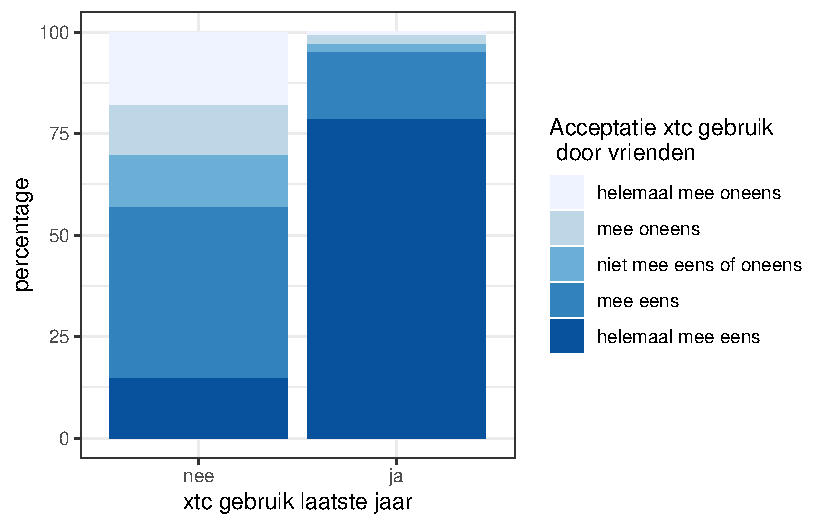
\includegraphics[keepaspectratio]{002-04-relatiesvariabelen_files/figure-pdf/unnamed-chunk-7-1.pdf}}

Wederom krijgen we direct een indruk van de relatie tussen deze twee
variabelen. Acceptie van xtc gebruik is over het algemeen hoog onder
vrienden, maar relatief veel meer bij vrienden van jongeren die zelf xtc
gebruiken.

Kruistabellen en (gestapelde) staafdiagrammen zijn ook goed toepasbaar
voor het onderzoeken van de relatie tussen twee ordinale variabelen (dit
behandelen we niet verder hier). Alleen als je variabelen heel veel
categorieën hebben, moet je wellicht nadenken over een alternatief.

\section{Kwalitatief
vs.~kwantitatief}\label{kwalitatief-vs.-kwantitatief}

We beschikken over verschillende opties wanneer we de relatie tussen een
kwalitatieve en kwantitatieve variabele willen onderzoeken. De meest
eenvoudige optie is om naar het verschil in gemiddeldes te kijken. Als
voorbeeld kijken we hier naar geslacht en het aantal sigaretten dat men
rookt tijdens het uitgaan (sigaretten\_uitgaansdag). Let op dat hier
alleen gaat over jongeren die minimaal één sigaret roken tijdens het
uitgaan (rokers).

We berekenen het gemiddelde door de data eerst te groeperen en daarna
het gemiddelde per groep te berekenen. Hoe je dat moet doen, leer je in
het practicum.

\begin{Shaded}
\begin{Highlighting}[]
\CommentTok{\# gemiddelde berekenen van van aantal sigaretten voor geslacht}
\NormalTok{data\_uitgaan }\SpecialCharTok{|\textgreater{}} \FunctionTok{group\_by}\NormalTok{(geslacht) }\SpecialCharTok{|\textgreater{}}
  \FunctionTok{filter}\NormalTok{(}\SpecialCharTok{!}\FunctionTok{is.na}\NormalTok{(sigaretten\_uitgaansdag)) }\SpecialCharTok{|\textgreater{}} \CommentTok{\# respondenten die niet roken eruit laten}
  \FunctionTok{summarise}\NormalTok{(}\AttributeTok{gem\_sigaretten =} \FunctionTok{mean}\NormalTok{(sigaretten\_uitgaansdag)) }\CommentTok{\# summarise() en mean() voor gemiddelde berekenen}
\end{Highlighting}
\end{Shaded}

\begin{verbatim}
# A tibble: 3 x 2
  geslacht gem_sigaretten
  <fct>             <dbl>
1 man                11.1
2 vrouw              11.2
3 anders             20  
\end{verbatim}

Je ziet dat zowel mannen als vrouwen gemiddeld zo'n 11 sigaretten per
uitgaansdag roken. Er is dus niet echt een verschil tussen deze groepen.
Bij de anders-identificerenden ligt dit aantal hoger (20), maar dit is
een kleine groep wat betekent dat het meer afhankelijk is van wie er
toevallig in de dataset zit.

Het verschil in gemiddeldes geeft nog niet zoveel inzicht in de
distributie van verschillende groepen. Het kan zijn dat er onderling
variatie is in het rookgedrag tussen mannen en vrouwen. Je kunt een
doosdiagram voor beide groepen maken om hier meer inzicht in te krijgen.

\begin{Shaded}
\begin{Highlighting}[]
\CommentTok{\# doosdiagram met aantal sigaretten naar geslacht}
\FunctionTok{ggplot}\NormalTok{(data\_uitgaan, }\FunctionTok{aes}\NormalTok{(}\AttributeTok{x =}\NormalTok{ geslacht, }\AttributeTok{y =}\NormalTok{ sigaretten\_uitgaansdag)) }\SpecialCharTok{+}
  \FunctionTok{geom\_boxplot}\NormalTok{() }\SpecialCharTok{+}
  \FunctionTok{theme\_bw}\NormalTok{() }\SpecialCharTok{+}
  \FunctionTok{ylab}\NormalTok{(}\StringTok{"aantal sigaretten uitgaansdag"}\NormalTok{) }
\end{Highlighting}
\end{Shaded}

\pandocbounded{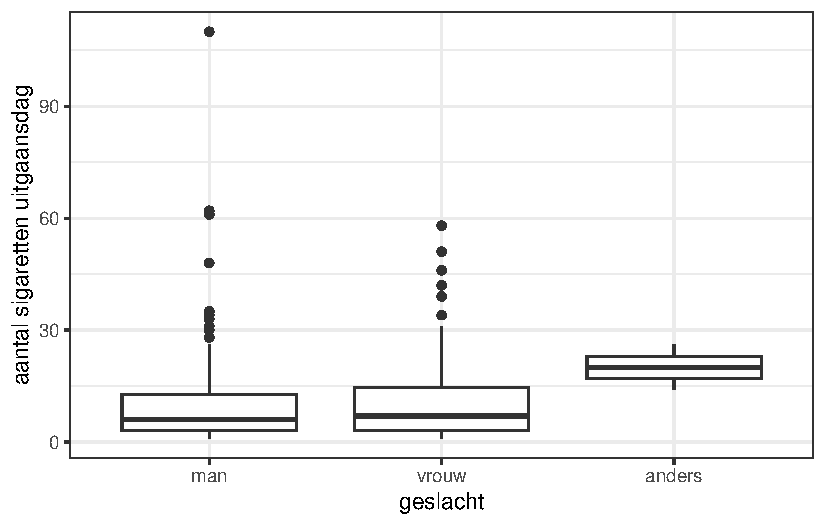
\includegraphics[keepaspectratio]{002-04-relatiesvariabelen_files/figure-pdf/unnamed-chunk-9-1.pdf}}

Deze doosdiagrammen zien er wat anders uit dan in hoofdstuk xxx, omdat
we hier met meer extreme waarden te maken hebben. Zo geeft de bovenste
punt bij de mannen aan dat één respondent meer dan 100 sigaretten heeft
gerookt. Gelet op de spreiding, is de afstand tussen Q1, Q2 en Q3 wat
groter bij vrouwen dan mannen. Het lijkt er dus op dat bij de mannen
meer extreme waarden voorkomen, terwijl bij de vrouwen er in het midden
van de verdeling (interkwartielafstand) wat meer spreiding is.

Ook hier geldt weer: het onderzoeken van een beschrijvende relatie
tussen ordinaal vs.~kwantitatief kan doorgaans op dezelfde wijze als bij
nominaal vs.~kwantitatief.

\section{Kwantitatief
vs.~kwantitatief}\label{kwantitatief-vs.-kwantitatief}

Als laatste onderzoeken we de relatie tussen twee kwantitatieve
variabelen. Het makkelijkst is om deze relatie direct te visualiseren
(later in de cursus kijken we naar correlatie, een associatiemaat voor
de sterkte van de relatie). We nemen de relatie tussen het aantal glazen
alcohol op een uitgaansdag (glazen\_alcohol\_uitgaansdag) en het aantal
gerookte sigaretten. Het gaat hier om jongeren die dus zowel alcohol
drinken als roken tijdens het uitgaan. Verder zijn dit twee ratio
variabelen (bedenk waarom).

Om de relatie te visualiseren, maken we eerst gebruik van een
spreidingsdiagram.

\begin{Shaded}
\begin{Highlighting}[]
\CommentTok{\# spreidingsdiagram met aantal glazen alcohol en sigaretten}
\FunctionTok{ggplot}\NormalTok{(data\_uitgaan, }\FunctionTok{aes}\NormalTok{(}\AttributeTok{x =}\NormalTok{ glazen\_alcohol\_uitgaansdag, }\AttributeTok{y =}\NormalTok{ sigaretten\_uitgaansdag)) }\SpecialCharTok{+}
  \FunctionTok{geom\_point}\NormalTok{() }\SpecialCharTok{+}
  \FunctionTok{theme\_bw}\NormalTok{() }\SpecialCharTok{+}
  \FunctionTok{xlab}\NormalTok{(}\StringTok{"aantal glazen alcohol uitgaansdag"}\NormalTok{) }\SpecialCharTok{+}
  \FunctionTok{ylab}\NormalTok{(}\StringTok{"aantal sigaretten uitgaansdag"}\NormalTok{)}
\end{Highlighting}
\end{Shaded}

\pandocbounded{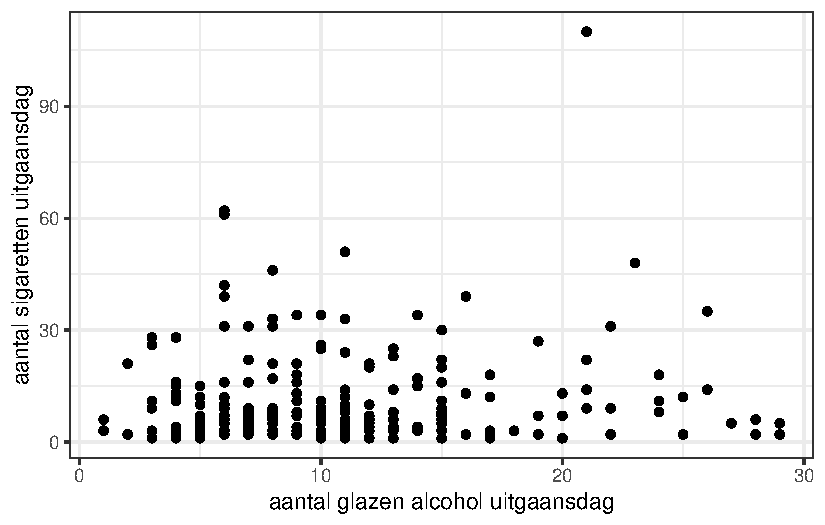
\includegraphics[keepaspectratio]{002-04-relatiesvariabelen_files/figure-pdf/unnamed-chunk-10-1.pdf}}

Elke punt vertegenwoordigd een respondent in deze diagram, die laat zien
hoe ze scoren op aantal glazen alcohol (x-as) en aantal sigaretten
(y-as) tijdens het uitgaan. Er komt hier nog niet een heel duidelijk
patroon uit naar voren. Zowel bij jongeren die relatief weinig drinken
(10\textless{} glazen) zijn er wat uitschieters naar boven qua roken
(\textgreater30 sigaretten), maar ook bij jongeren die relatief veel
drinken. De dichste concentratie van punten zit linksonder, wat betekent
dat de meeste respondenten rond de 5-15 glazen alcohol drinken en 1-15
sigaretten roken.

We kunnen de spreidingsdiagram nog wat aanpassen om beter inzicht te
krijgen in de relatie. Sommige punten zijn nu niet goed te zien omdat ze
dicht op elkaar zitten. Met die optie ``\emph{jitter''} wordt de
puntenwolk wat meer uitgespreid.

\begin{Shaded}
\begin{Highlighting}[]
\CommentTok{\# spreidingsdiagram met aantal glazen alcohol en sigaretten}
\FunctionTok{ggplot}\NormalTok{(data\_uitgaan, }\FunctionTok{aes}\NormalTok{(}\AttributeTok{x =}\NormalTok{ glazen\_alcohol\_uitgaansdag, }\AttributeTok{y =}\NormalTok{ sigaretten\_uitgaansdag)) }\SpecialCharTok{+}
  \FunctionTok{geom\_point}\NormalTok{(}\AttributeTok{position =} \StringTok{"jitter"}\NormalTok{) }\SpecialCharTok{+} \CommentTok{\# jitter toevoegen}
  \FunctionTok{theme\_bw}\NormalTok{() }\SpecialCharTok{+}
  \FunctionTok{xlab}\NormalTok{(}\StringTok{"aantal glazen alcohol uitgaansdag"}\NormalTok{) }\SpecialCharTok{+}
  \FunctionTok{ylab}\NormalTok{(}\StringTok{"aantal sigaretten uitgaansdag"}\NormalTok{)}
\end{Highlighting}
\end{Shaded}

\pandocbounded{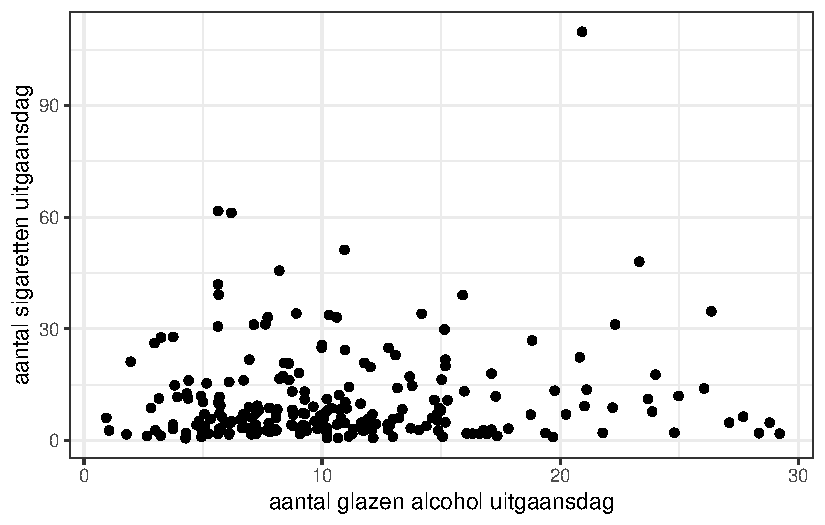
\includegraphics[keepaspectratio]{002-04-relatiesvariabelen_files/figure-pdf/unnamed-chunk-11-1.pdf}}

Je ziet nu iets beter waar de concentratie van datapunten zit. Verder
kun je kijken in hoeverre er een (lineair) verband is tussen aantal
glazen alcohol en aantal sigaretten. Je kunt een zogenoemde
regressielijn `fitten' op de data met \emph{stat\_smooth().}

\begin{Shaded}
\begin{Highlighting}[]
\CommentTok{\# spreidingsdiagram met aantal glazen alcohol en sigaretten}
\FunctionTok{ggplot}\NormalTok{(data\_uitgaan, }\FunctionTok{aes}\NormalTok{(}\AttributeTok{x =}\NormalTok{ glazen\_alcohol\_uitgaansdag, }\AttributeTok{y =}\NormalTok{ sigaretten\_uitgaansdag)) }\SpecialCharTok{+}
  \FunctionTok{geom\_point}\NormalTok{(}\AttributeTok{position =} \StringTok{"jitter"}\NormalTok{) }\SpecialCharTok{+}
  \FunctionTok{theme\_bw}\NormalTok{() }\SpecialCharTok{+}
  \FunctionTok{xlab}\NormalTok{(}\StringTok{"aantal glazen alcohol uitgaansdag"}\NormalTok{) }\SpecialCharTok{+}
  \FunctionTok{ylab}\NormalTok{(}\StringTok{"aantal sigaretten uitgaansdag"}\NormalTok{) }\SpecialCharTok{+}
  \FunctionTok{stat\_smooth}\NormalTok{(}\AttributeTok{method =}\NormalTok{ loess, }\AttributeTok{se =} \ConstantTok{FALSE}\NormalTok{)}
\end{Highlighting}
\end{Shaded}

\pandocbounded{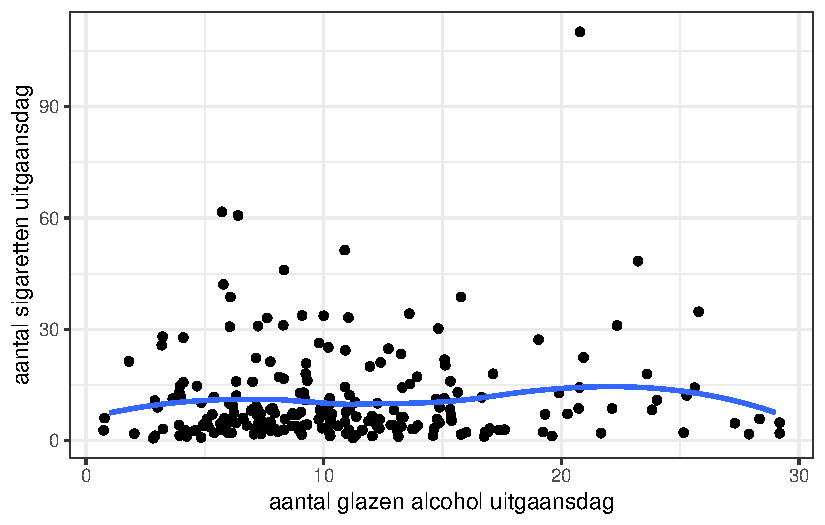
\includegraphics[keepaspectratio]{002-04-relatiesvariabelen_files/figure-pdf/unnamed-chunk-12-1.pdf}}

De lijn toont dat er geen duidelijk verband is tussen aantal glazen
alcohol en aantal sigaretten. Over het algemeen blijft deze vrij vlak en
gaat niet duidelijk één richting op.

\section{Tot slot}\label{tot-slot}

Dit hoofdstuk heeft geïllustreerd hoe je relaties tussen variabelen kan
beschrijven, zowel door tabellen en visualisaties. Daarbij is het
belangrijk om het meetniveau van beide variabelen te weten. Besteed ook
aandacht aan de interpretatie: waaraan kun je aflezen hoe een bepaalde
relatie in elkaar zit? Daarvan zijn enkele voorbeelden gegeven. Zo weet
je na dit hoofdstuk bijvoorbeeld:

\begin{itemize}
\tightlist
\item
  Dat vrouwen iets vaker vapen dan mannen
\item
  Acceptatie onder vrienden van xtc hoger is onder gebruikers dan
  niet-gebruikers
\item
  Mannen en vrouwen gemiddeld evenveel roken, maar de onderlinge
  variatie net wat anders is
\item
  Er geen duidelijke relatie is tussen het aantal glazen alcohol dat men
  drinkt en aantal sigaretten dat men rookt op een uitgaansdag
\end{itemize}

\part{Steekproeven en betrouwbaarheidsinterval}

\chapter{Inferentie en steekproeven}\label{inferentie-en-steekproeven}

\section{Populatie en steekproef}\label{populatie-en-steekproef}

We zijn tot nu toe met beschrijvende statistiek bezig geweest. Je hebt
nu een idee hoe we data kunnen samenvatten en visualiseren, en hoe we de
relaties tussen variabelen kunnen analyseren. Dit zijn nuttige skills
voor de rest van de cursus en (wellicht) ook voor later in je carrière
als criminoloog.

We hebben ons in de vorige hoofdstukken gericht op de xxx respondenten
die in de dataset zitten. Hoewel interessant, vertelt dit ons nog vrij
weinig over de bredere populatie van uitgaande jongeren. Terwijl dit
juist het centrale doel is van statistisch onderzoek: op basis van een
steekproef willen we uitspraken doen die voor deze gehele populatie
gelden! Dit noemen we ook wel \textbf{inferentie}, of
\textbf{inferentiële statistiek}. Om dit te begrijpen, is het handig de
begrippen populatie en steekproef kort uit te leggen.

\textbf{Populatie}: De complete groep van analyse-eenheden waarin we
geïnteresseerd zijn. In de criminologie gaat dit vaak om personen in een
groep die we zo helder mogelijk proberen te identificeren en af te
bakenen. Bijvoorbeeld alle leden van criminele motorclub of
smokkelnetwerk. In deze cursus richten we ons in principe op alle
jongeren in Nederland die weleens op stap gaan.

\textbf{Steekproef}: Een willekeurige selectie van eenheden uit de
populatie. Willekeurige selectie betekent dat iedereen evenveel kans
heeft om onderdeel te zijn van de steekproef (\emph{random sample}). De
steekproef is daarmee in principe een representatieve afspiegeling is
van de populatie. De steekproef bestaat uit onze observaties in de
dataset, in dit geval alle jongeren die de vragenlijst hebben ingevuld.

Het idee achter inferentie is eigenlijk vrij simpel. In de praktijk is
het vaak lastig om data over de hele populatie te verzamelen. We kunnen
onmogelijk alle uitgaande jongeren in Nederland interviewen, dat gaat om
miljoenen mensen! Toch willen we iets zinnigs kunnen zeggen over deze
populatie. Bijvoorbeeld over het aandeel jongeren dat een bepaalde drugs
gebruikt. Op basis van statistische kennis weten we dat we met slechts
een klein deel van die jongeren (de steekproef) toch met bepaalde
zekerheid (en onder bepaalde assumpties) iets kunnen zeggen over de
populatie als geheel.

Dit brengt echter de nodige uitdagingen met zich mee. Hoe kun je de
gegevens uit de steekproef gebruiken om iets te zeggen over de
populatie, en hoe weet je zeker dat dit vervolgens klopt? En welke
assumpties maken we daarbij? Dit omvat vele aspecten van meetmethode en
statistiek. Daar gaan we in dit hoofdstuk verder op in. Ook zullen we
tijdens de onderwijsgroepen en colleges hier meer bij stilstaan. Het is
echter goed te realiseren dat we niet al deze complexiteit kunnen
behandelen.

\section{Steekproevenverdeling en centrale
limietstelling}\label{sec-steekproefcentraallimiet}

Stel, we willen weten welk aandeel uitgaande jongeren in Nederland
weleens xtc heeft gebruikt. Daarvoor kunnen we een proportie berekenen:
welk aandeel jongeren van het totaal aantal het betreft. Ons doel is
hier om de proportie xtc-gebruikers in de Nederlandse populatie van
uitgaande jongeren te \emph{schatten} (bij benadering), we zullen immers
nooit zeker weten wat deze precieze proportie is. Daar zouden we alle
uitgaande jongeren in de populatie voor moeten bevragen.

Een proportie is een voorbeeld van een \textbf{parameter}: een
kwantiteit die we schatten die ons informatie geeft over de populatie.
Dit kan een proportie zijn, maar bijvoorbeeld ook een gemiddelde of een
correlatie.

We geven eerst kort wat notatie. We zijn geïnteresseerd in wat de
proportie xtc-gebruikers is in de populatie uitgaande jongeren, deze
populatieparameter noteren we als \(P\) . Omdat we deze parameter niet
direct weten, nemen we een steekproef van jongeren uit deze populatie.
De proportie xtc-gebruikers in deze steekproef wordt genoteerd als
\(\hat{p}\).\footnote{Hetzelfde principe geldt voor andere parameters
  waarin we mogelijk geinteresseerd zijn. Als je het gemiddelde van een
  populatie (\(\mu\)) wil schatten, trek je daarvoor een steekproef die
  uiteraard ook zijn eigen gemiddelde heeft (\(\bar{x}\))}

Om het proces van het schatten van de populatieparameter \(P\)
(proportie xtc-gebruikers) uit te leggen, doen we geheel volgens
wetenschappelijke traditie een klein gedachte-experiment, maar deze keer
ook met praktische toepassing. Voor dit experiment doen we alsof we wel
data voor de gehele populatie hebben. In dit geval is deze populatie
alle jongeren die onze dataset zitten (wat origineel de steekproef was).
We berekenen eerst de proportie \(P\) voor deze populatie.

\begin{Shaded}
\begin{Highlighting}[]
\CommentTok{\# proportie xtc{-}gebruikers berekenen}
\FunctionTok{table}\NormalTok{(data\_uitgaan}\SpecialCharTok{$}\NormalTok{xtc\_ooit) }\SpecialCharTok{|\textgreater{}} \FunctionTok{prop.table}\NormalTok{()}
\end{Highlighting}
\end{Shaded}

\begin{verbatim}

      nee        ja 
0.3150289 0.6849711 
\end{verbatim}

We zien dat deze proportie 0,685 bedraagt, oftewel 68,5\% van de
uitgaande jongeren heeft ooit xtc geprobeerd.

Voor het gedachte-experiment gaan we er even vanuit dat we de proportie
van de populatie niet kennen, maar juist willen schatten. Daarom trekken
we uit de populatie een steekproef van 30 personen. Vervolgens berekenen
we daarvoor de proportie xtc-gebruikers \(\hat{p}\) .

\begin{Shaded}
\begin{Highlighting}[]
\CommentTok{\# set.seed() om voorbeeld te reproduceren}
\FunctionTok{set.seed}\NormalTok{(}\DecValTok{010}\NormalTok{)}

\CommentTok{\# steekproef trekken van 30 personen uit populatie}
\NormalTok{sample\_30 }\OtherTok{\textless{}{-}} \FunctionTok{slice\_sample}\NormalTok{(data\_uitgaan, }\AttributeTok{n =} \DecValTok{30}\NormalTok{)}

\CommentTok{\# proportie xtc{-}gebruikers berekenen}
\FunctionTok{table}\NormalTok{(sample\_30}\SpecialCharTok{$}\NormalTok{xtc\_ooit) }\SpecialCharTok{|\textgreater{}} \FunctionTok{prop.table}\NormalTok{()}
\end{Highlighting}
\end{Shaded}

\begin{verbatim}

      nee        ja 
0.3448276 0.6551724 
\end{verbatim}

We zien dat voor deze steekproef van 30 personen de proportie 0,655 is
(65,5\%). Dit lijkt dus op de populatie proportie \(P\) van 0,685, maar
er zit wel een klein verschil tussen (0,685 - 0,655 = 0,030; 3,0\% om
precies te zijn).

Dit verschil tussen \(P\) en \(\hat{p}\) treedt in principe altijd op
bij een willekeurige steekproef en de grootte ervan varieert per genomen
steekproef. Laten we dit nader te bekijken. We trekken nu tien
willekeurige steekproeven van 30 personen en berekenen alle
steekproefproporties van xtc gebruikers.

\begin{Shaded}
\begin{Highlighting}[]
\FunctionTok{set.seed}\NormalTok{(}\DecValTok{010}\NormalTok{)}

\CommentTok{\# 10 keer een steekproef van 30 trekken en de proportie xtc{-}gebruikers berekenen}
\NormalTok{proporties\_xtc }\OtherTok{\textless{}{-}} \FunctionTok{replicate}\NormalTok{(}\DecValTok{10}\NormalTok{, \{}
\NormalTok{  sample\_30 }\OtherTok{\textless{}{-}} \FunctionTok{slice\_sample}\NormalTok{(data\_uitgaan, }\AttributeTok{n =} \DecValTok{30}\NormalTok{)}
  \FunctionTok{mean}\NormalTok{(sample\_30}\SpecialCharTok{$}\NormalTok{xtc\_ooit }\SpecialCharTok{==} \StringTok{"ja"}\NormalTok{, }\AttributeTok{na.rm =} \ConstantTok{TRUE}\NormalTok{) }\CommentTok{\# na.rm om eventuele missenden waarden te verwijderen}
\NormalTok{\})}

\CommentTok{\# proporties bekijken}
\FunctionTok{print}\NormalTok{(proporties\_xtc)}
\end{Highlighting}
\end{Shaded}

\begin{verbatim}
 [1] 0.6551724 0.6666667 0.7586207 0.7333333 0.5333333 0.8000000 0.6666667
 [8] 0.6896552 0.7586207 0.5862069
\end{verbatim}

Je ziet dat sommige proporties \(\hat{p}\) vrij dicht bij \(P\) liggen
(bijvoorbeeld 0,690) terwijl anderen er ver weg van liggen (0,533). We
zien dus dat er variatie is tussen steekproeven in de proporties.

Een uitgangspunt van inferentiële statistiek is dat een steekproef één
mogelijke uitkomst is van een denkbeeldig universum met een oneindig
aantal uitkomsten. Deze uitkomsten zijn willekeurige variaties op een
onderliggende `ware' populatieparameter (in dit geval \(P\)). Als we
steekproeven oneindig zouden blijven herhalen, dan zal uiteindelijk het
gemiddelde van alle mogelijke uitkomsten deze ware populatieparameter
weergeven. Dit omdat eventuele afwijkingen het gevolg zijn van
willekeurige variatie.

Als je hoofd inmiddels begint te duizelen, geen paniek. We komen hier
later meer op terug. Ook zullen we vooral kijken naar wat dit in
praktijk betekent.

Zoals je wellicht kunt voorstellen, is het logisch niet mogelijk om
oneindig steekproeven te blijven trekken. Daarom doen we dat hier bij
benadering door `slechts' 10.000 steekproeven te trekken van 30
personen.

\begin{Shaded}
\begin{Highlighting}[]
\FunctionTok{set.seed}\NormalTok{(}\DecValTok{010}\NormalTok{)}

\CommentTok{\# 10 keer een steekproef van 30 trekken en de proportie xtc{-}gebruikers berekenen}
\NormalTok{proporties\_xtc\_10k }\OtherTok{\textless{}{-}} \FunctionTok{replicate}\NormalTok{(}\DecValTok{10000}\NormalTok{, \{}
\NormalTok{  sample\_30 }\OtherTok{\textless{}{-}} \FunctionTok{slice\_sample}\NormalTok{(data\_uitgaan, }\AttributeTok{n =} \DecValTok{30}\NormalTok{)}
  \FunctionTok{mean}\NormalTok{(sample\_30}\SpecialCharTok{$}\NormalTok{xtc\_ooit }\SpecialCharTok{==} \StringTok{"ja"}\NormalTok{, }\AttributeTok{na.rm =} \ConstantTok{TRUE}\NormalTok{) }\CommentTok{\# na.rm om eventuele missenden waarden te verwijderen}
\NormalTok{\})}
\end{Highlighting}
\end{Shaded}

Vervolgens visualiseren we de proporties xtc-gebruikers van al deze
steekproeven in een histogram, en berekenen we enkele centrum- en
spreidingsmaten.

\begin{Shaded}
\begin{Highlighting}[]
\CommentTok{\# histogram maken}
\FunctionTok{ggplot}\NormalTok{(}\FunctionTok{as.data.frame}\NormalTok{(proporties\_xtc\_10k), }
       \FunctionTok{aes}\NormalTok{(}\AttributeTok{x =}\NormalTok{ proporties\_xtc\_10k)) }\SpecialCharTok{+}
  \FunctionTok{geom\_histogram}\NormalTok{(}\AttributeTok{bins =} \DecValTok{22}\NormalTok{, }\AttributeTok{fill =} \StringTok{"grey"}\NormalTok{, }\AttributeTok{colour =} \StringTok{"black"}\NormalTok{) }\SpecialCharTok{+}  
  \FunctionTok{theme\_bw}\NormalTok{() }\SpecialCharTok{+}
  \FunctionTok{ylab}\NormalTok{(}\StringTok{"aantal steekproeven"}\NormalTok{) }\SpecialCharTok{+}
  \FunctionTok{xlab}\NormalTok{ (}\StringTok{"proporties xtc{-}gebruikers"}\NormalTok{)}
\end{Highlighting}
\end{Shaded}

\pandocbounded{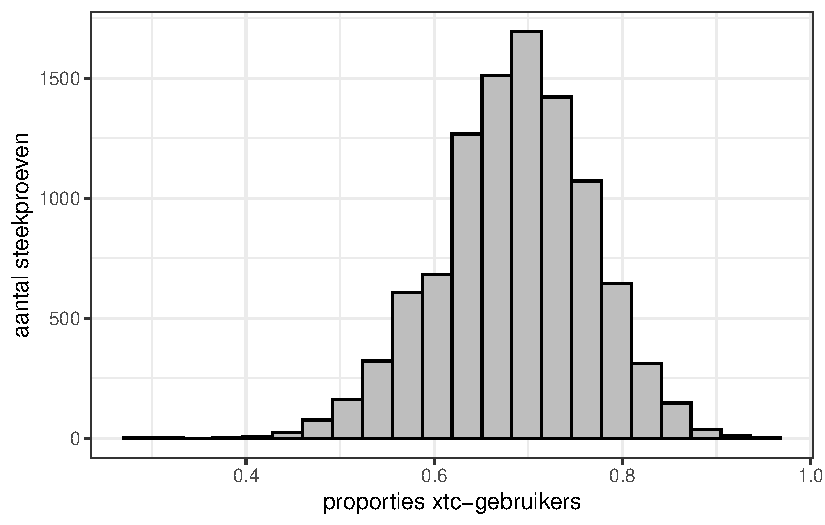
\includegraphics[keepaspectratio]{003-01-steekproeven_files/figure-pdf/unnamed-chunk-6-1.pdf}}

\begin{Shaded}
\begin{Highlighting}[]
\CommentTok{\# berekenen centrum{-} en spreidingsmaten}
\FunctionTok{summary}\NormalTok{(proporties\_xtc\_10k)}
\end{Highlighting}
\end{Shaded}

\begin{verbatim}
   Min. 1st Qu.  Median    Mean 3rd Qu.    Max. 
 0.3000  0.6333  0.6897  0.6849  0.7333  0.9667 
\end{verbatim}

\begin{Shaded}
\begin{Highlighting}[]
\FunctionTok{sd}\NormalTok{(proporties\_xtc\_10k)}
\end{Highlighting}
\end{Shaded}

\begin{verbatim}
[1] 0.08147867
\end{verbatim}

Wat je hierboven ziet, staat ook wel bekend als de
\textbf{steekproevenverdeling}. Dat wil zeggen, de verdeling van de
mogelijke uitkomsten (hier: proporties) van herhaalde steekproeven (in
dit geval: 10.000 steekproeven van 30 personen betreffende de proportie
xtc-gebruikers).

Er vallen een paar dingen op als we bovenstaande gegevens kijken. Ten
eerste lijkt de verdeling van steekproefproporties nagenoeg op een
normale verdeling, zoals we eerder hebben gezien
(\hyperref[sec-normaleverdeling]{Normale verdeling}). Dit betekent dat
de steekproevenverdeling dezelfde eigenschappen heeft als een normale
verdeling, zoals dat het kansverdeling is (we kunnen de kans op een
bepaalde uitkomst berekenen) en dat het een gemiddelde en een
standaarddeviatie heeft. Je kunt verder zien dat het gemiddelde van
0,685 nagenoeg gelijk is aan de mediaan van 0,690, wat verder indiceert
dat we hier met een normale verdeling te maken hebben (symmetrie). Het
minimum (0,300) en maximum (0,967) tonen verder bij enkele steekproeven
de proportie juist ver af zit van het populatiegemiddelde, maar de
verdeling toont tevens dat dit uitzonderlijke uitkomsten zijn.

Het meest interessant is echter dat de steekproevenverdeling van
proporties allesbehalve willekeurig is. Het resulteert immers in een
normale verdeling! En dat niet alleen: de gemiddelde proportie van de
steekproevenverdeling (\(\bar{x}_\hat{p}=0,685\)) is afgerond gelijk aan
het populatiegemiddelde (\(P=0,685\)). In het algemeen geldt dan ook dat
het gemiddelde van de steekproevenverdeling gelijk is aan het
populatiegemiddelde.

Hoe komt dat? Stel dat je een steekproef trekt met een selectie personen
die op alle denkbare kenmerken gelijk zijn aan alle personen in de
populatie. Het is met andere woorden een perfecte afspiegeling van de
populatie. In dit geval vind je dat \(P=\hat{p}\) . Dit is echter bijna
nooit het geval. Omdat een steekproef willekeurig wordt getrokken, zul
je bijna altijd toevallige afwijkingen hebben. Dat je bijvoorbeeld net
iets meer xtc-gebruikers selecteert dan niet-gebruikers ten opzichte van
de verhouding in de populatie, wat weer invloed heeft op de hoogte van
de proportie xtc-gebruikers. Maar, ervan uitgaande dat elke afwijking
willekeurig is, zal bij oneindige herhaling van steekproeven het
gemiddelde van alle afwijkingen 0 zijn (het is immers willekeurig of je
een hogere of lagere proportie krijgt in een steekproef).

Een ander interessant gegeven is dat de steekproevenverdeling naast een
gemiddelde zijn eigen standaarddeviatie heeft. Dit is een speciale
variant van de standaarddeviatie, en wordt de \textbf{standaardfout}
genoemd. Deze noteren we als \(\sigma_{\hat{p}}\). \footnote{goed om te
  weten: het aantal observaties (respondenten) in de steekproef noteren
  we met \(n\); het aantal eenheden (personen) in de populatie noteren
  we met \(N\)} De `fout' geeft dus eigenlijk aan in hoeverre een
steekproefuitkomst (proportie v/d steekproef) afwijkt van de
populatieparameter (proportie v/d de populatie). De standaardfout is
belangrijk omdat we deze, zoals we later zullen zien, kunnen gebruiken
om te berekenen wat de foutmarge van onze steekproef is met betrekking
tot het schatten van de populatieparameter.

Knoop het dus goed in je oren: \emph{de standaardfout is de
standaarddeviatie van de steekproevenverdeling}. Deze noteren we
bijvoorbeeld als \(\sigma_{\hat{p}}\) voor proporties en
\(\sigma_{\bar{x}}\) voor gemiddeldes.

Dit is wat anders dan de gebruikelijke standaarddeviatie, die gaat om
originele variabelen in de dataset die iets proberen te meten
(bijvoorbeeld leeftijd of gemoedstoestand op dinsdag)

Wat we zojuist hebben aangetoond, is de \textbf{centrale
limietstelling}. Deze houdt in dat:

\begin{itemize}
\tightlist
\item
  Als een oneindig aantal willekeurige steekproeven bestaat uit ongeveer
  30 observaties of meer, dan\ldots{}
\item
  Is het gemiddelde van de steekproevenverdeling gelijk aan het
  populatiegemiddelde
\item
  Is de steekproevenverdeling normaal verdeeld, met eigen standaardfout
\item
  Zelfs als de oorspronkelijke variabele niet normaal verdeeld is!
  (zoals bijvoorbeeld xtc\_gebruik\_ooit; dit is een dichotome
  variabele)
\end{itemize}

De regels rondom de centrale limietstelling zijn net wet anders bij
minder dan 30 observaties, zie daarvoor bijvoorbeeld \emph{Statistiek
als hulpmiddel} of het internet.

Doordat we de standaardfout kennen, kunnen we in combinatie met
\hyperref[sec-normaleverdeling]{de empirische regel} bepalen hoe
waarschijnlijk een bepaalde (willekeurige) steekproefuitkomst voorkomt.
Daar gaan we zo mee verder. Eerst laten we de magie van de
steekproevenverdeling en centrale limietstelling even op ons inwerken.

\pandocbounded{\includegraphics[keepaspectratio]{afbeeldingen/Mind_blown.gif}}

\section{Één steekproef en de standaardfout}\label{sec-standaardfout}

Degenen die een beetje bij zijn gekomen van het conceptueel geweld
hierboven (en wellicht ook degenen voor wie de verwarring compleet is),
zullen wellicht inmiddels aan het denken zijn: ja dat is allemaal leuk
en aardig die 10.000 steekproeven, maar in de praktijk helemaal niet
werkbaar. We kunnen immers niet voor elk onderzoek 10.000 steekproeven
uitvoeren, dat kost tijd en geld en na de eerste steekproef is de lol er
eigenlijk ook wel een beetje vanaf.

Gelukkig is hier een eenvoudige oplossing voor. Het blijkt namelijk
statistisch zo te zijn dat we de standaardfout kunnen berekenen op basis
van één steekproef. We hoeven dus helemaal geen 10.000 steekproeven te
trekken om de standaardfout te berekenen!

Voor een het berekenen van de standaardfout van proporties
\(\sigma_{\hat{p}}\) geldt\footnote{Voor het berekenen van de
  standaardfout van steekproefgemiddeldes \(\sigma_{\bar{x}}\) geldt een
  andere formule (zie \href{formuleblad.qmd}{Formuleblad})}:

\[\sigma_{\hat{p}}=\sqrt\frac{\hat{p}(1-\hat{p})}{n}\]

In deze formule zie je dat de proportie van de steekproef \(\hat{p}\)
wordt vermenigvuldigd met \((1-\hat{p})\) , vervolgens gedeeld door het
aantal observaties in de steekproef \(n\) en daar de wortel van wordt
genomen.\footnote{Goed om te weten: het aantal observaties
  (respondenten) in de steekproef noteren we met \(n\); het aantal
  eenheden (personen) in de populatie noteren we met \(N\)}

Dat de \(n\) in deze formule in de noemer staat (onder de streep) heeft
een belangrijke implicatie. Dit betekent namelijk dat hoe meer data we
verzamelen voor een steekproef (het aantal observaties), hoe kleiner de
standaardfout wordt. En met een kleinere standaardfout kunnen we weer
meer exact de populatieparameter schatten! (komen we later nog op terug)

Laten we dit even illustreren aan de hand van een voorbeeld. We
selecteren willekeurig 10, 30, en 100 mensen uit de dataset, wat
neerkomt op steekproeven met een verschillend aantal observaties. Ook
berekenen we de standaardfout voor de gehele dataset (xxx respondenten).

\begin{Shaded}
\begin{Highlighting}[]
\FunctionTok{set.seed}\NormalTok{(}\DecValTok{010}\NormalTok{)}

\CommentTok{\# Functie om de standaardfout van een proportie te bereknen}
\NormalTok{se\_proportie }\OtherTok{\textless{}{-}} \ControlFlowTok{function}\NormalTok{(x) \{}
\NormalTok{  x }\OtherTok{\textless{}{-}} \FunctionTok{na.omit}\NormalTok{(x)}
\NormalTok{  p }\OtherTok{\textless{}{-}} \FunctionTok{mean}\NormalTok{(x }\SpecialCharTok{==} \StringTok{"ja"}\NormalTok{)}
  \FunctionTok{sqrt}\NormalTok{(p }\SpecialCharTok{*}\NormalTok{ (}\DecValTok{1} \SpecialCharTok{{-}}\NormalTok{ p) }\SpecialCharTok{/} \FunctionTok{length}\NormalTok{(x))}
\NormalTok{\}}

\CommentTok{\# Steekproeven trekken van 10, 30 en 100 respondenten}
\NormalTok{steekproef\_10  }\OtherTok{\textless{}{-}} \FunctionTok{slice\_sample}\NormalTok{(data\_uitgaan, }\AttributeTok{n =} \DecValTok{10}\NormalTok{)}
\NormalTok{steekproef\_30  }\OtherTok{\textless{}{-}} \FunctionTok{slice\_sample}\NormalTok{(data\_uitgaan, }\AttributeTok{n =} \DecValTok{30}\NormalTok{)}
\NormalTok{steekproef\_100 }\OtherTok{\textless{}{-}} \FunctionTok{slice\_sample}\NormalTok{(data\_uitgaan, }\AttributeTok{n =} \DecValTok{100}\NormalTok{)}

\CommentTok{\# Standaardfouten berekenen}
\FunctionTok{se\_proportie}\NormalTok{(steekproef\_10}\SpecialCharTok{$}\NormalTok{xtc\_ooit) }\CommentTok{\# 10 respondenten}
\end{Highlighting}
\end{Shaded}

\begin{verbatim}
[1] 0.1656347
\end{verbatim}

\begin{Shaded}
\begin{Highlighting}[]
\FunctionTok{se\_proportie}\NormalTok{(steekproef\_30}\SpecialCharTok{$}\NormalTok{xtc\_ooit) }\CommentTok{\# 30 respondenten}
\end{Highlighting}
\end{Shaded}

\begin{verbatim}
[1] 0.083666
\end{verbatim}

\begin{Shaded}
\begin{Highlighting}[]
\FunctionTok{se\_proportie}\NormalTok{(steekproef\_100}\SpecialCharTok{$}\NormalTok{xtc\_ooit) }\CommentTok{\# 100 respondenten}
\end{Highlighting}
\end{Shaded}

\begin{verbatim}
[1] 0.04661037
\end{verbatim}

\begin{Shaded}
\begin{Highlighting}[]
\FunctionTok{se\_proportie}\NormalTok{(data\_uitgaan}\SpecialCharTok{$}\NormalTok{xtc\_ooit) }\CommentTok{\# xxx respondenten (complete dataset)}
\end{Highlighting}
\end{Shaded}

\begin{verbatim}
[1] 0.02497315
\end{verbatim}

Je ziet dus dat de standaardfout steeds kleiner wordt naarmate we een
grotere steekproef hebben. Bij 10 respondenten is de standaardfout nog
0,16; bij xxx respondenten is deze 0,02. Dit toont dat, als de
assumpties kloppen, meer data meer beter is.

\section{Assumpties (the mother of
all\ldots)}\label{assumpties-the-mother-of-all}

Je hebt het al een paar keer voorbij horen komen: onder bepaalde
assumpties kunnen we ervan uitgaan dat een schatting van de
populatieparameter klopt.\footnote{Kleine waarschuwing: wat nu volgt kan
  de eerste keer een beetje pijn doen aan je brein.} Maar wat zijn die
assumpties? In de statistiek gaan we hier vaak makkelijk aan voorbij of
kijken we er liever van weg, waarschijnlijk omdat de waarheid wat
ongemakkelijk is en ook ingewikkeld. We hechten er echter veel waarde
aan dat je toch op de hoogte bent van enkele assumpties. Omdat je
daardoor beter begrijpt wat je wel en niet kan met statistiek. En dat je
uiteindelijk hopelijk kritischer zal kijken naar veel statistieken die
je in het dagelijks leven voorbij ziet komen.

\subsection{Willekeurige en systematische
fouten}\label{willekeurige-en-systematische-fouten}

Een eerste belangrijke assumptie is dat eventuele afwijkingen/fouten in
de steekproef willekeurig zijn (\textbf{willekeurige fout}; \emph{random
error} in het Engels). Dit hebben we al deels besproken in dit
hoofdstuk. Er zal altijd een zekere mate van toeval zijn bij het trekken
van steekproef. Zolang dit een willekeurige afwijking betreft, is er
niet zoveel aan de hand. We weten immers wat de kans is op een bepaalde
mate van toeval (hoever een steekproefuitkomst van \(P\) of \(\mu\) kan
liggen) en kunnen daarmee rekening houden bij het schatten van de
populatieparameter.

Helaas komt het in steekproefonderzoek vaak voor dat fouten niet
willekeurig zijn, maar eerder systematisch van aard. Dit kan op diverse
wijzen gebeuren en zullen we daarom niet uitputtend behandelen hier. We
geven een aantal voorbeelden om dit te verhelderen.

Een type \textbf{systematische fout} (\emph{systematic error}) is dat je
selectie van respondenten niet willekeurig is omdat er een structurele
afwijking in zit. Dit kan zijn omdat een bepaalde groep binnen de
populatie waar je in geïnteresseerd bent om een specifieke reden niet
deelneemt aan onderzoek. Jongeren die een problematische hoeveelheid xtc
gebruiken, zullen vaker vermoeid zijn en wellicht mentale problemen
hebben. Daardoor zullen ze minder snel meedoen aan surveyonderzoek
vanwege een gebrek aan focus of andere prioriteiten. Wanneer deze groep
systematisch ondervertegenwoordigd is in je steekproef, zul je de
proportie xtc-gebruikers (en ook de frequentie van gebruik) steeds te
laag in schatten. Hoe vaak je ook een steekproef afneemt! Het voorkomen
van dit soort systematische fouten is erg lastig en vergt goede kennis
van de doelpopulatie en goed zicht op het proces van dataverzameling.

Een ander type systematisch fout kan in de vragenlijst zelf zitten. Stel
dat die groep problematische en hoog-frequente gebruikers wel meedoet
aan je onderzoek, maar in de vragenlijst hun gebruik stelselmatig
onderrapporteert. Dat ze in hun antwoorden aangeven minder te gebruiken
dan ze daadwerkelijk doen, vanwege sociale wenselijkheid of schaamte.
Dan schat je het gebruik nog steeds te laag in.

\subsection{Willekeurige selectie}\label{willekeurige-selectie}

Bij het verzamelen van steekproefdata zijn er verder diverse praktische
uitdagingen. Het idee van een willekeurig getrokken steekproef
(\emph{random sample}) veronderstelt dat je een overzicht heb van je
populatie (alle uitgaande jongeren in Nederland tussen de 16 en 35 jaar)
en vervolgens potentiële respondenten op willekeurige wijze selecteert.
Maar hoe krijg je dat overzicht, het gaat immers om honderdduizenden zo
niet miljoenen personen? Je zou bijvoorbeeld kunnen beginnen bij het
willekeurig selecteren van plekken in Nederland (steden en dorpen),
vervolgens een aantal uitgaansgelegenheden willekeurig selecteren
(cafés, kroegen, discotheken, festivals, etc.) en dan op die plekken
willekeurig jongeren benaderen om mee te doen aan het onderzoek. Je kunt
je voorstellen dat dit laatste al lastig genoeg is: hoe ga je in drukke
discotheek willekeurig mensen benaderen? Nog los van het gegeven dat
sommige mensen te veel onder invloed zijn om een vragenlijst serieus in
te vullen.

In het oorspronkelijke onderzoek
(\href{https://www.trimbos.nl/kennisbank/rapport-het-grote-uitgaansonderzoek-2023/}{Het
Grote Uitgaansonderzoek}), waar onze dataset op is gebaseerd, is de
werving van respondenten via social media gegaan. Het Trimbos instituut
heeft via advertenties en een wervingscampagne respondenten geworven via
Instagram, Snapchat en Facebook. Hoewel dit geschikte platformen zijn om
uitgaande jongeren te bereiken, is de selectie van respondenten
allesbehalve willekeurig. In plaats van willekeurig te selecteren uit de
populatie is het proces hier eerder andersom: je stuurt een bericht de
wereld in om te kijken wie uit de populatie er mee wil doen aan het
onderzoek. Ook zal niet iedereen uit de doelpopulatie op deze platformen
zitten (mensen zonder social media).

Dit wil niet zeggen dat het onderzoek geen zin heeft of meteen niet
valide is. Het gaat er eerder om dat we ons bewust zijn van de
beperkingen en mogelijke fouten, zodat we geen onjuiste uitspraken doen
op basis van de data en onze methoden. In theorie stellen we dat als de
selectie van respondenten totaal willekeurig plaatsvindt, dat er geen
systematische fouten zijn op basis van zowel geobserveerde (variabelen
die we meten) en niet-geobserveerde kenmerken (wat we niet meten in de
vragenlijst). In de praktijk is het vaak wat rommeliger.

De hier genoemde fouten hebben te maken met de \textbf{validiteit} en
\textbf{betrouwbaarheid} van kwantitatief onderzoek. Dit zijn
belangrijke aspecten waar we in de colleges en onderwijsgroepen ook meer
aandacht aan zullen besteden.

\subsection{De constante
populatieparameter}\label{de-constante-populatieparameter}

Naast mogelijke systematische fouten zijn de filosofische aannames
achter statistiekonderzoek niet altijd even goed toepasbaar. Zoals
eerder gesteld is het idee achter de dominante manier van statistiek
bedrijven dat er zoiets bestaat als een ware populatieparameter \(P\)
die we in theorie kunnen achterhalen door een oneindig aantal
onderzoeken (bijvoorbeeld experimenten of steekproeven) uit te voeren.
Er wordt aangenomen dat de populatieparameter een constante, vaste
waarde heeft. Als we onderzoek blijven herhalen, krijgen we steeds net
wat andere data door willekeurige fouten. De data varieert dus, de
populatieparameter niet. Op de lange termijn zal het gemiddelde van al
deze onderzoeken echter leiden tot de ware \(P\) (zie
Section~\ref{sec-steekproefcentraallimiet}). Dit denken gaat dus uit van
soort denkbeeldig universum waarin we deze onderzoeken oneindig kunnen
herhalen. In de praktijk voeren we het onderzoek vaak eenmaal uit.

In sommige situaties is deze manier van denken geschikt. Als we
geïnteresseerd zijn in xtc-gebruik onder uitgaande jongeren in
Nederland, kunnen we ervan uitgaan dat in er in deze populatie een
zekere constante proportie van gebruik bestaat. Bij herhaalde
onderzoeken zullen we dan los van toevallige fouten naar verwachting min
of meer steeds op dezelfde proportie uitkomen (zie het voorbeeld onder
Section~\ref{sec-steekproefcentraallimiet}), althans op de korte tot
middellange termijn. Over de tijd zal het gebruik als het gevolg van
maatschappelijke en culturele veranderingen variëren.

Voor meer specifieke vragen geeft de aanname van een universum met een
ware populatieparameter die we ontdekken door oneindig herhaalde
onderzoeken wel problemen (lees deze zin gerust nog een keer). Neem als
voorbeeld dat we geïnteresseerd zijn in de proportie xtc-gebruikers op
het festival Lowlands in 2026. Dit is een eenmalig evenement. We kunnen
er wellicht van uitgaan dat er zoiets is als een constante
populatieparameter `proportie xtc-gebruik' voor dit festival, maar we
kunnen in de praktijk geen herhaalde onderzoeken blijven doen om dit te
meten. Deze editie van 2026, waar we specifiek in zijn geïnteresseerd,
vind immers maar één keer plaats en we kunnen dus ook maar één keer
onderzoek doen. De statistiekfilosofie laat ons hier in de steek.

Dat de filosofie niet helemaal kloppend is voor de onderzoekspraktijk is
niet per se een probleem, onderzoek vergt wel vaker wat conceptueel
rekwerk. Desalniettemin moeten we ons goed rekenschap geven van deze
assumpties.

\section{Samenvatting}\label{samenvatting-1}

Je hersenen zullen vast een beetje kraken na dit hoofdstuk. In essentie
komt het erop neer dat:

\begin{itemize}
\tightlist
\item
  In inferentie proberen we een populatieparameter (proportie
  xtc-gebruik onder uitgaande jongeren) te schatten middels een
  willekeurig getrokken steekproef.
\item
  Middels de steekproevenverdeling kunnen we berekenen hoe groot de kans
  is op een afwijkende steekproefproportie ten opzichte van de proportie
  in de populatie, met behulp van de standaardfout
\item
  Aan de hand van één steekproef kunnen we de standaardfout verkrijgen,
  waarbij geldt dat deze kleiner wordt bij een grotere steekproef
\item
  Er zijn diverse fouten mogelijk bij een steekproef waar we ons bewust
  van moeten zijn
\end{itemize}

\chapter{Betrouwbaarheidsinterval}\label{betrouwbaarheidsinterval}

We zijn in het vorige hoofdstuk ingegaan op de principes van
inferentiële statistiek, de steekproevenverdeling, de standaardfout,
assumpties en mogelijke fouten die kunnen plaatsvinden.

We moeten nu een volgende stap maken, namelijk die van het trekken van
één steekproef naar het schatten van de populatieparameter. Omdat we
nooit helemaal zeker weten wat de populatieparameter is, schatten we met
behulp van de standaardfout hoe dicht we in de buurt zitten (de
foutmarge). Dit doen we aan de hand van een
\textbf{betrouwbaarheidsinterval} (afkorting: bhi). We zullen in dit
hoofdstuk in een aantal concrete stappen laten we zien we hoe dit doen.

\section{Betrouwbaarheidsinterval voor
proporties}\label{betrouwbaarheidsinterval-voor-proporties}

\subsection{Denkbeeldig voorbeeld}\label{denkbeeldig-voorbeeld}

We beginnen met een denkbeeldig voorbeeld. We gaan er net als bij het
vorige hoofdstuk vanuit dat we het populatieproportie en de
standaardfout al kennen van xtc-gebruik onder uitgaande jongeren,
waarbij we de dataset als populatie beschouwen. Dit is uiteraard zelden
het geval (daarom doen we onderzoek!), maar voor de uitleg die volgt is
dit wel handig.

Als we volgens de centrale limietstelling oneindig steekproeven trekken
van 30 personen, willen we weten wat het bereik is van 95\% van de
steekproefuitkomsten (proporties in dit geval) rondom het
populatiegemiddelde. Met 95\% hebben we een aardig beeld van wat voor
proporties de meeste steekproeven zouden opleveren. Dat is hieronder
gevisualiseerd.

\pandocbounded{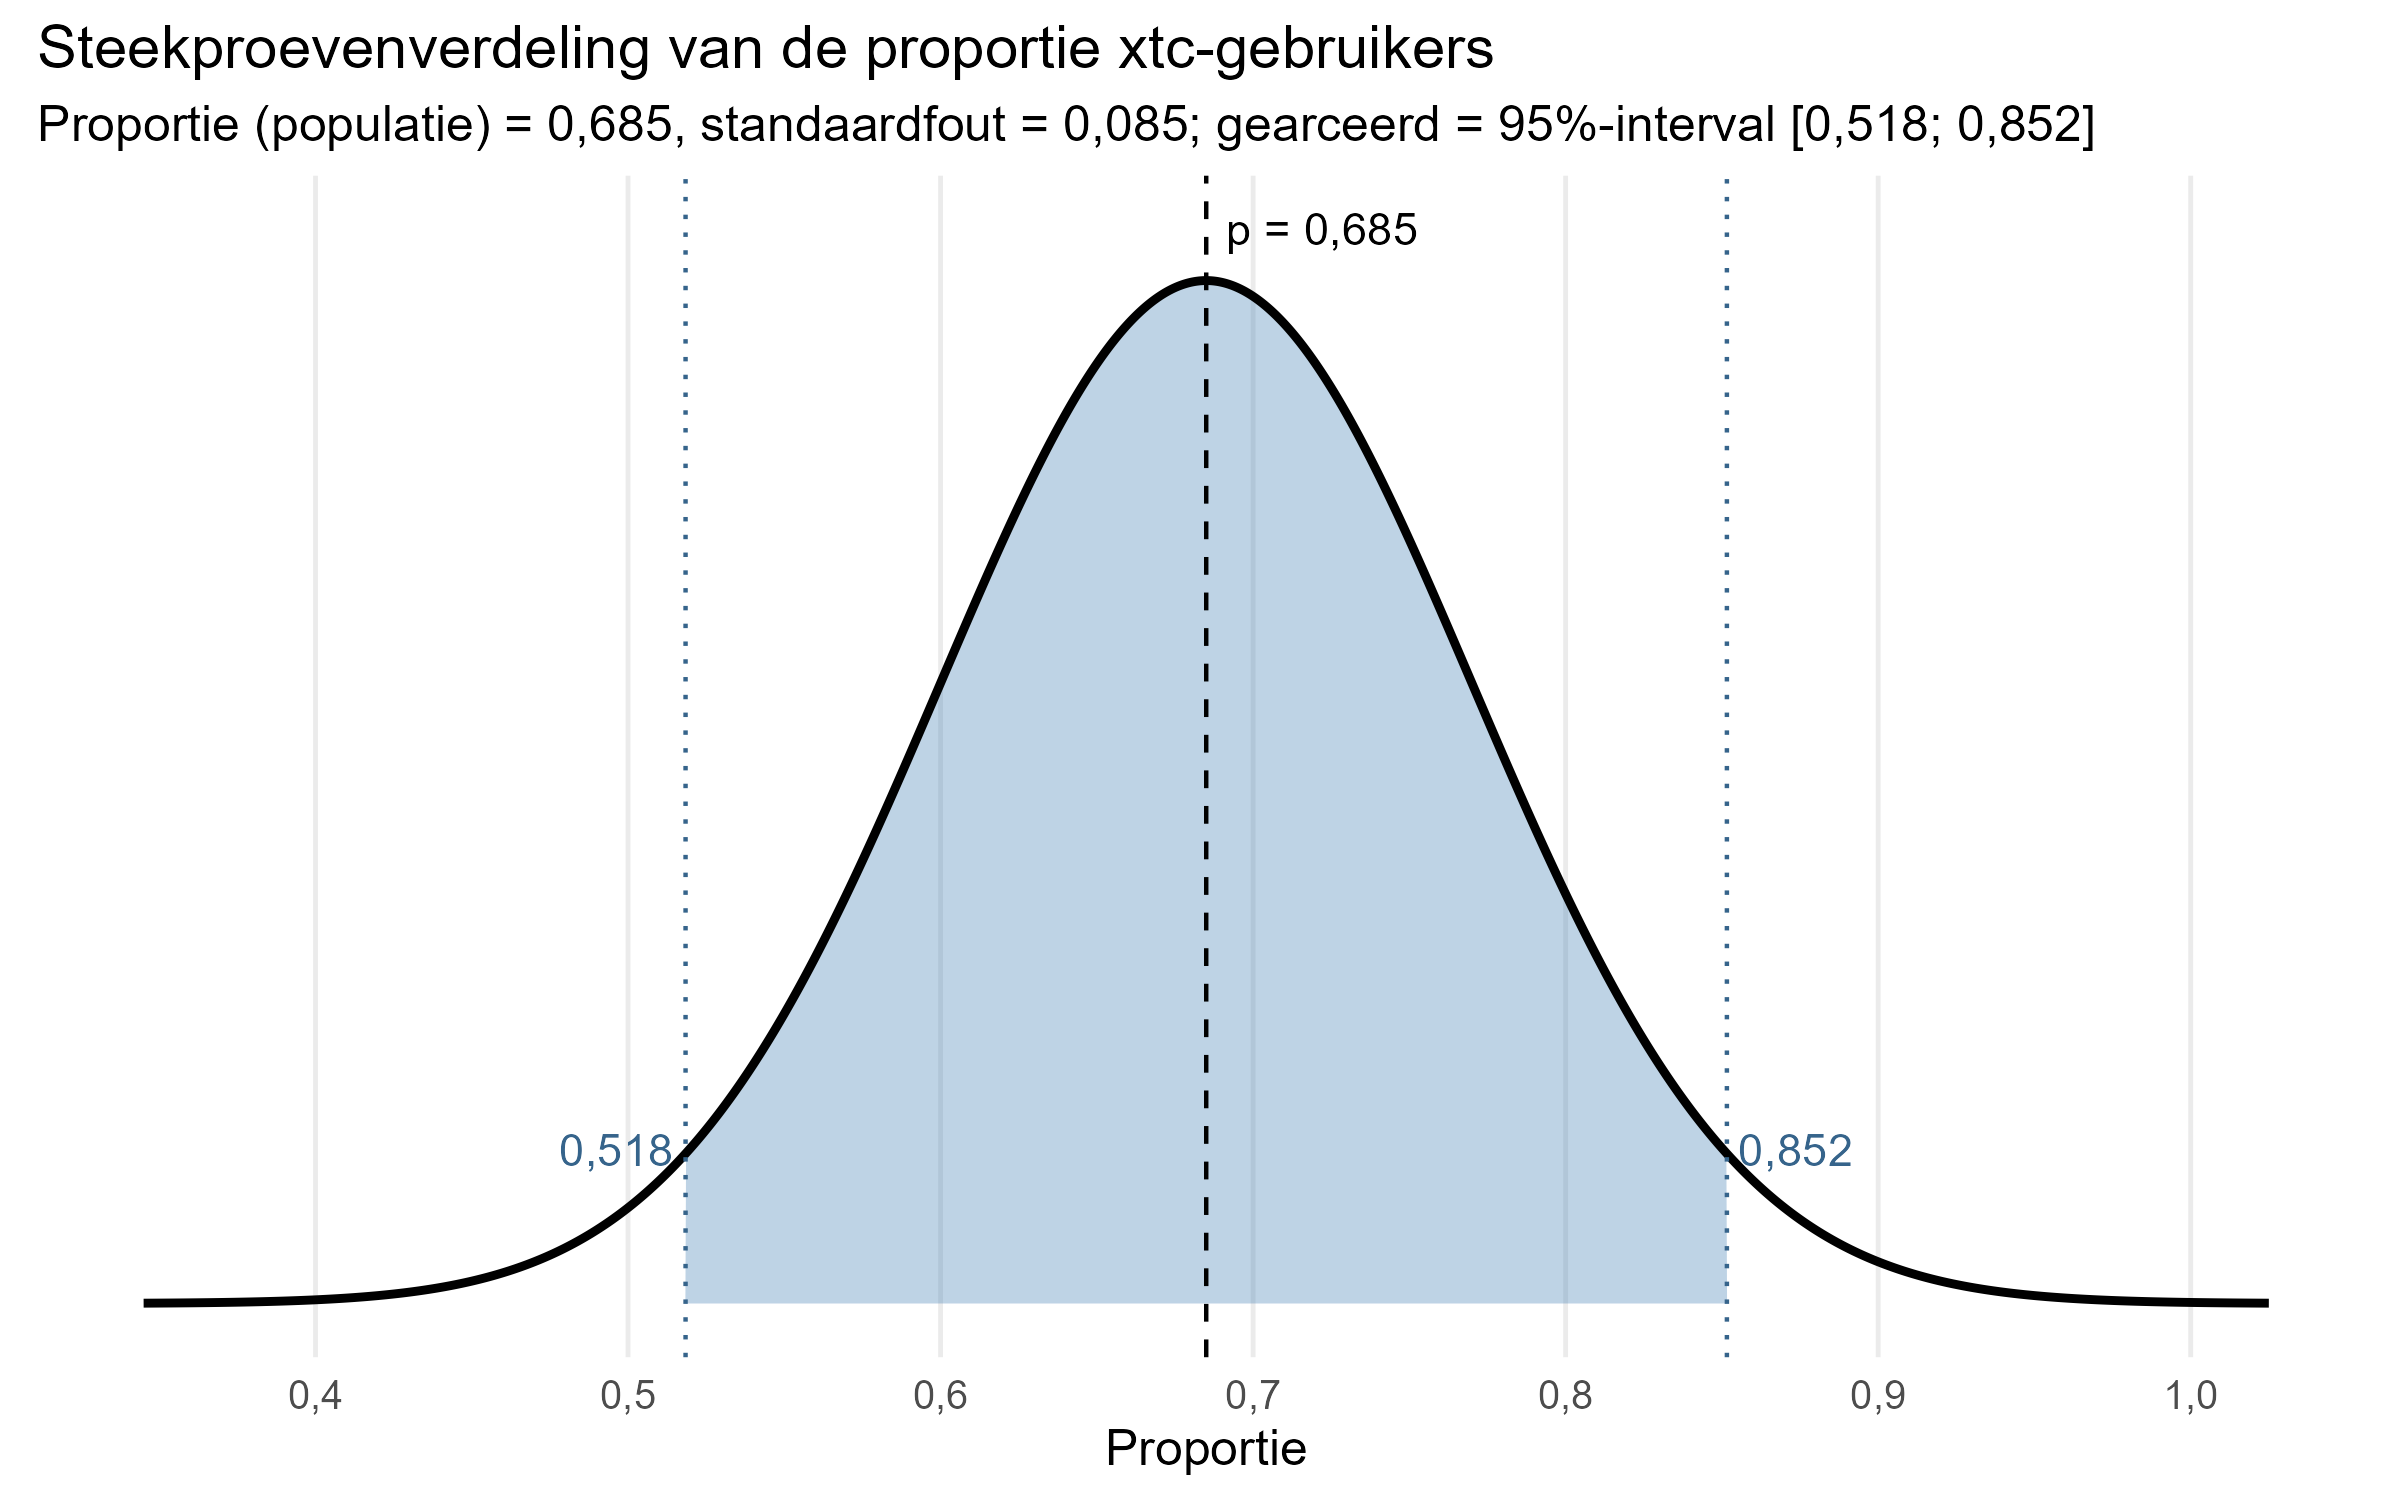
\includegraphics[keepaspectratio]{afbeeldingen/normal_distribution.png}}

De afbeelding hierboven is afgeleid van het
\hyperref[sec-steekproefcentraallimiet]{voorbeeld} uit het vorige
hoofdstuk. Het toont dat we als herhaalde steekproeven zouden doen
waarbij de proportie in de populatie van xtc-gebruik 0,685 is, dat 95\%
van de steekproeven een proportie tussen de 0,518 en 0,852 zou
opleveren.

Waarom kiezen we hier voor 95\%? Dat is afgeleid uit de empirische regel
die we bij de \hyperref[sec-normaleverdeling]{Normale verdeling} hebben
besproken. Daar zag je bijvoorbeeld dat 95,4\% van alle observaties
tussen 2 standaarddeviaties boven en onder het midden van de verdeling
liggen. 95\% wordt vaak als conventioneel interval gebruikt, omdat het
een breed interval betreft dat veel mogelijke uitkomsten bevat zonder
dat het betekenisloos wordt.\footnote{Andere veelgebruikte
  betrouwbaarheidsintervallen zijn 90\% en 99\%. De bijbehorende
  standaarddeviaties zijn hierbij respectievelijk 1,65 en 2,58 (op basis
  van z-scores).} Het 95\%-betrouwbaarheidsinterval correspondeert met
1,96 standaarddeviaties boven en onder het midden van de verdeling.

Aan de hand van de formule van betrouwbaarheidsinterval kunnen we zien
hoe we dit berekenen:

\[
bhi = P \pm z\times\sigma_{\hat{p}} 
\]

of:

\[bhi \enspace ondergrens = P - z\times\sigma_{\hat{p}}\]

\[bhi \enspace bovengrens = P + z\times\sigma_{\hat{p}}\]

Je neemt dus:

\begin{itemize}
\tightlist
\item
  de (schatting van de) populatieparameter \(P\)
\item
  telt daarbij op en trekt af de standaarddeviatie \(z\) die je hebt
  gekozen voor de grens van het bhi. De \(z\) komt van de
  (gestandaardiseerde standaarddeviaties) die je eerder hebt gezien.
\item
  De \(z\) moet je wel eerst vermenigvuldigen met de standaardfout
  \(\sigma_{\hat{p}}\)
\end{itemize}

We weten voor dit voorbeeld dat:

\begin{itemize}
\item
  \(P=0,685\)
\item
  \(z=1,96\) (we hebben gekozen voor een 95\%-bhi)
\end{itemize}

Je hebt eerder gezien hoe je de
\hyperref[sec-standaardfout]{standaardfout} berekent voor proporties. Je
hoeft alleen de proportie en aantal respondenten in te vullen:

\[\sigma_{\hat{p}}=\sqrt\frac{\hat{p}(1-\hat{p})}{n}=\sqrt\frac{0,685(1-0,685)}{30}\]

\begin{Shaded}
\begin{Highlighting}[]
\CommentTok{\# berekenen standaardfout voor voorbeeld}
\FunctionTok{sqrt}\NormalTok{(}\FloatTok{0.685}\SpecialCharTok{*}\NormalTok{(}\DecValTok{1}\FloatTok{{-}0.685}\NormalTok{)}\SpecialCharTok{/}\DecValTok{30}\NormalTok{)}
\end{Highlighting}
\end{Shaded}

\begin{verbatim}
[1] 0.08480861
\end{verbatim}

De standaardfout is in dit geval dus 0,085.

Dan hoeven we in principe alleen nog de formule van het bhi in te
vullen:

\[
bhi = P \pm z\times\sigma_{\hat{p}} = 0,685 \pm 1,96\times0,085
\]

We berekenen eerst het deel achter de \(\pm\)
(\(z\times\sigma_{\hat{p}}\) ):

\begin{Shaded}
\begin{Highlighting}[]
\CommentTok{\# gedeelte achter +{-}}
\FloatTok{1.96}\SpecialCharTok{*}\FloatTok{0.085}
\end{Highlighting}
\end{Shaded}

\begin{verbatim}
[1] 0.1666
\end{verbatim}

Dit is dus 0,167. Het bereik van het 95\%-bhi ligt 0,167 boven en onder
de populatieproportie van 0,685. Dit tellen we op/trekken we af van
0,685.

\begin{Shaded}
\begin{Highlighting}[]
\CommentTok{\# berekenen bhi}
\FloatTok{0.685{-}0.167} \CommentTok{\# ondergrens}
\end{Highlighting}
\end{Shaded}

\begin{verbatim}
[1] 0.518
\end{verbatim}

\begin{Shaded}
\begin{Highlighting}[]
\FloatTok{0.685+0.167} \CommentTok{\# bovengrens}
\end{Highlighting}
\end{Shaded}

\begin{verbatim}
[1] 0.852
\end{verbatim}

Voilà! We weten nu dus dat als we oneindig willekeurige steekproeven
zouden trekken van 30 personen uit een populatie uitgaande jongeren, dat
de proporties xtc-gebruik in 95\% van de steekproeven tussen de 0,518 en
0,852 zouden liggen (als overige assumpties kloppen).

\subsection{Reëel voorbeeld}\label{reuxebel-voorbeeld}

Het denkbeeldige voorbeeld is instructief, maar eigenlijk overbodig. We
gingen er al vanuit dat de proportie in de populatie 0,685 was. Dan is
het in principe niet meer nodig een betrouwbaarheidsinterval te
berekenen.

We weten nu echter ook het volgende: omdat 95\% van de verdeling van
mogelijke steekproefproporties tussen 0,518 en 0,852 ligt (0,167 boven
of onder 0,685), is de kans 95\% dat een proportie van een willekeurige
steekproef binnen dit bereik valt. Dit betekent dat als we herhaaldelijk
een proportie \(\hat{p}\) berekenen op basis van een willekeurige
steekproef (van 30 personen in dit geval), en vervolgens een interval
berekenen tussen \(\hat{p}-0,167\) en \(\hat{p}+0,167\) , dat dit
interval de populatieproportie zal bevatten in 95\% van de steekproeven.

Simpel gezegd, kunnen we in de formule
\(bhi = P \pm z\times\sigma_{\hat{p}}\) de \(P\) vervangen door
\(\hat{p}\), en dan voor elke steekproef berekenen in welk interval de
populatieparameter mogelijk ligt. We zullen daarbij ook de standaardfout
\(\sigma_{\hat{p}}\) opnieuw moeten berekenen, omdat die we berekend
hebben aan de hand van \(P=0,685\) maar die kennen we in de
werkelijkheid niet. De nieuwe formule voor het schatten van een
betrouwbaarheidsinterval is:

\[ bhi = \hat{p} \pm z\times\sigma_{\hat{p}}  \]

of:

\[bhi \enspace ondergrens = \hat{p} - z\times\sigma_{\hat{p}}\]

\[bhi \enspace bovengrens = \hat{p} + z\times\sigma_{\hat{p}}\]

We kunnen nu zien hoe dit werkt aan de hand van een voorbeeld. We
trekken een steekproef van 30 personen en berekenen de proportie
xtc-gebruikers in deze steekproef.

\begin{Shaded}
\begin{Highlighting}[]
\FunctionTok{set.seed}\NormalTok{(}\DecValTok{42}\NormalTok{)}

\CommentTok{\# steekproef trekken van 30 personen uit populatie}
\NormalTok{sample\_30 }\OtherTok{\textless{}{-}} \FunctionTok{slice\_sample}\NormalTok{(data\_uitgaan, }\AttributeTok{n =} \DecValTok{30}\NormalTok{)}

\CommentTok{\# proportie xtc{-}gebruikers berekenen}
\FunctionTok{table}\NormalTok{(sample\_30}\SpecialCharTok{$}\NormalTok{xtc\_ooit) }\SpecialCharTok{|\textgreater{}} \FunctionTok{prop.table}\NormalTok{()}
\end{Highlighting}
\end{Shaded}

\begin{verbatim}

      nee        ja 
0.3666667 0.6333333 
\end{verbatim}

De proportie xtc-gebruikers in deze steekproef is dus 0,633. Eerst
berekenen we de nieuwe standaardfout:

\[\sigma_{\hat{p}}=\sqrt\frac{\hat{p}(1-\hat{p})}{n}=\sqrt\frac{0,633(1-0,633)}{30}\]

\begin{Shaded}
\begin{Highlighting}[]
\CommentTok{\# berekenen standaardfout voor willekeurige steekproef met 30 respondenten}
\FunctionTok{sqrt}\NormalTok{(}\FloatTok{0.633}\SpecialCharTok{*}\NormalTok{(}\DecValTok{1}\FloatTok{{-}0.633}\NormalTok{)}\SpecialCharTok{/}\DecValTok{30}\NormalTok{)}
\end{Highlighting}
\end{Shaded}

\begin{verbatim}
[1] 0.0879983
\end{verbatim}

De standaardfout is 0,088. Dan hebben we alle relevante gegevens om het
95\%-betrouwbaarheidsinterval te berekenen:

\[
bhi = \hat{p} \pm z\times\sigma_{\hat{p}} = 0,633 \pm 1,96\times0,088
\]

\begin{Shaded}
\begin{Highlighting}[]
\CommentTok{\# gedeelte achter +{-}}
\FloatTok{1.96}\SpecialCharTok{*}\FloatTok{0.088}
\end{Highlighting}
\end{Shaded}

\begin{verbatim}
[1] 0.17248
\end{verbatim}

\begin{Shaded}
\begin{Highlighting}[]
\CommentTok{\# berekenen bhi}
\FloatTok{0.633{-}0.172} \CommentTok{\# ondergrens}
\end{Highlighting}
\end{Shaded}

\begin{verbatim}
[1] 0.461
\end{verbatim}

\begin{Shaded}
\begin{Highlighting}[]
\FloatTok{0.633+0.172} \CommentTok{\# bovengrens}
\end{Highlighting}
\end{Shaded}

\begin{verbatim}
[1] 0.805
\end{verbatim}

De ondergrens van het 95\%-bhi is in dit geval 0,461 en de bovengrens is
0,805. Dit noteren we ook wel als \([0,461; 0,805]\). Op basis hiervan
concluderen we (voorlopig) dat in 95\% van de herhaalde steekproeven de
populatieproportie tussen deze twee waarden zou moeten liggen. In dit
geval is dat correct: 0,685 ligt tussen 0,461 en 0,805.

Het principe van een 95\%-bhi is hieronder uitgebeeld. Deze grafiek
toont een simulatie waarin we 100 keer een steekproef hebben getrokken
van 30 personen en voor elke steekproef het 95\%-bhi hebben berekend.
Wanneer een interval de populatieproportie bevat, dan overlapt het
interval (horizontale grijze streep) met de verticale gestippelde lijn
die de populatieproportie presenteert. In 5\% van de steekproeven zie je
dat het interval en de populatieproportie niet overlappen. Dit zijn
steekproeven die toevallig een hele hoge of lage proportie van
xtc-gebruikers hebben (rode kleur). Uitgaande van een 95\%-bhi, valt de
populatiewaarde dan buiten het interval bij deze steekproeven. We zitten
er dus ook weleens naast met een steekproef, ook al is aan alle
assumpties voldaan. Het voordeel is wel dat we weten hoe vaak we er
naast zaten, namelijk in 5\% procent van de steekproeven.

\pandocbounded{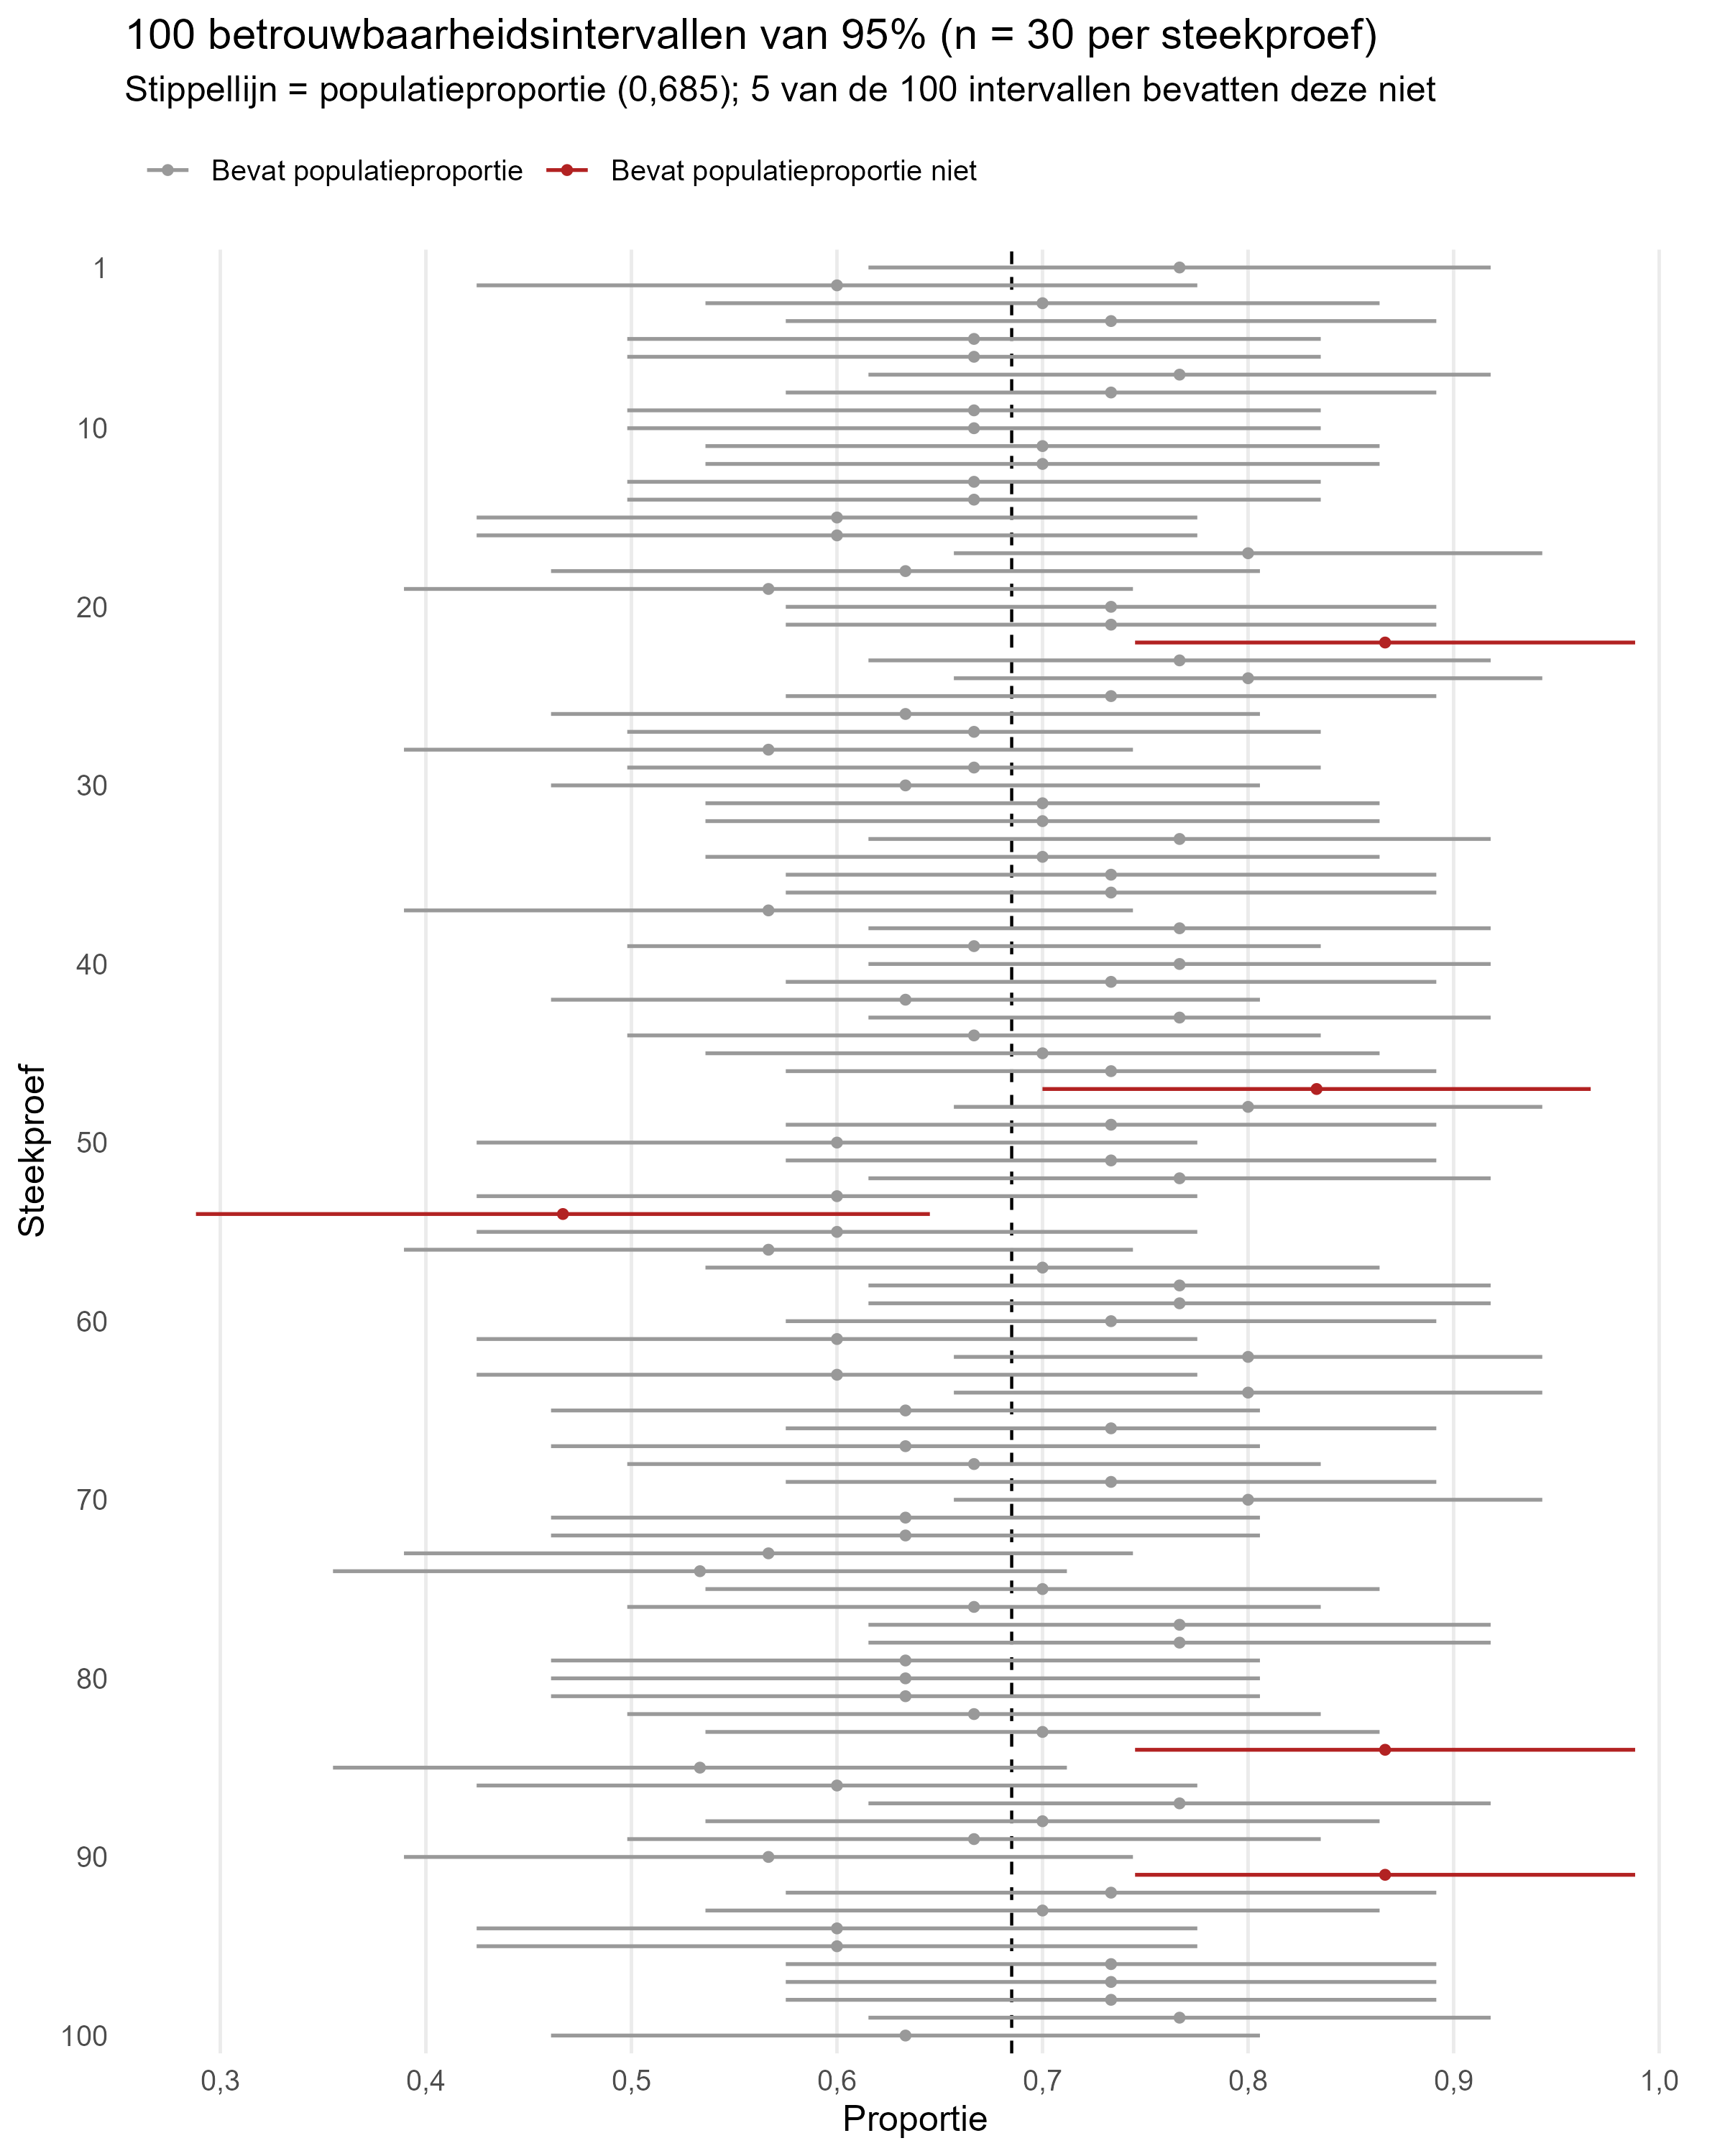
\includegraphics[keepaspectratio]{afbeeldingen/simulatie_betrouwbaarheidsintervallen.png}}

\subsection{Reëel voorbeeld \#2}\label{sec-reeelvoorbeeld2}

Hopelijk heb je inmiddels een beetje feeling gekregen voor
betrouwbaarheidsintervallen. Het vorige voorbeeld was leerzaam, maar de
uitkomst was een beetje teleurstellend. Dat we op basis van een
steekproef van 30 personen weten dat in 95\% van de steekproeven de
populatieproportie xtc-gebruikers ergens tussen de 0,461 en 0,805 ligt
is nog niet zo informatief. Het kan namelijk 0,461 zijn, of 0,805, of
alles daar tussen in. Het maakt nogal uit of het 46,1\% gebruikers gaat
of om 80,5\%! Stel je voor dat de media een bericht schrijft over jouw
onderzoek, dan wil je toch wat nauwkeuriger kunnen zeggen hoeveel
uitgaande jongeren ooit xtc hebben gebruikt.

We gaan nu kijken hoe de grootte van de steekproef hier van invloed is
(zie ook het deel over de \hyperref[sec-standaardfout]{standaardfout}).
We trekken nu geen steekproef van 30 personen, maar één van 10 en één
van 100 personen. Eerst schrijven we even een functie om het 95\%-bhi
automatisch te berekenen, zodat we niet alles weer stap voor stap hoeven
te berekenen.

\begin{Shaded}
\begin{Highlighting}[]
\CommentTok{\# functie schrijven voor 95\%{-}bhi}
\NormalTok{bhi\_95 }\OtherTok{\textless{}{-}} \ControlFlowTok{function}\NormalTok{(p, n) \{}
\NormalTok{  p }\SpecialCharTok{+} \FunctionTok{c}\NormalTok{(}\SpecialCharTok{{-}}\DecValTok{1}\NormalTok{, }\DecValTok{1}\NormalTok{) }\SpecialCharTok{*} \FloatTok{1.96} \SpecialCharTok{*} \FunctionTok{sqrt}\NormalTok{(p }\SpecialCharTok{*}\NormalTok{ (}\DecValTok{1} \SpecialCharTok{{-}}\NormalTok{ p) }\SpecialCharTok{/}\NormalTok{ n)}
\NormalTok{\}}
\end{Highlighting}
\end{Shaded}

We trekken twee steekproeven van respectievelijk 10 en 100 personen, en
berekenen de proporties.

\begin{Shaded}
\begin{Highlighting}[]
\FunctionTok{set.seed}\NormalTok{(}\DecValTok{42}\NormalTok{)}

\CommentTok{\# steekproeven trekken van 10 en 100 personen}
\NormalTok{sample\_10 }\OtherTok{\textless{}{-}} \FunctionTok{slice\_sample}\NormalTok{(data\_uitgaan, }\AttributeTok{n =} \DecValTok{10}\NormalTok{)}
\NormalTok{sample\_100 }\OtherTok{\textless{}{-}} \FunctionTok{slice\_sample}\NormalTok{(data\_uitgaan, }\AttributeTok{n =} \DecValTok{100}\NormalTok{)}

\CommentTok{\# proportie xtc{-}gebruikers berekenen}
\FunctionTok{table}\NormalTok{(sample\_10}\SpecialCharTok{$}\NormalTok{xtc\_ooit) }\SpecialCharTok{|\textgreater{}} \FunctionTok{prop.table}\NormalTok{() }\CommentTok{\# 10 personen}
\end{Highlighting}
\end{Shaded}

\begin{verbatim}

nee  ja 
0.3 0.7 
\end{verbatim}

\begin{Shaded}
\begin{Highlighting}[]
\FunctionTok{table}\NormalTok{(sample\_100}\SpecialCharTok{$}\NormalTok{xtc\_ooit) }\SpecialCharTok{|\textgreater{}} \FunctionTok{prop.table}\NormalTok{() }\CommentTok{\# 100 personen}
\end{Highlighting}
\end{Shaded}

\begin{verbatim}

      nee        ja 
0.4183673 0.5816327 
\end{verbatim}

De proportie voor de steekproef met 10 personen bedraagt 0,700 en die
voor 100 personen is 0,582. Nu berekenen we het 95\%-bhi voor beide
steekproeven.

\begin{Shaded}
\begin{Highlighting}[]
\CommentTok{\# 95\%{-}bhi berekenen voor beide steekproeven}
\FunctionTok{bhi\_95}\NormalTok{(}\FloatTok{0.7}\NormalTok{, }\DecValTok{10}\NormalTok{) }\CommentTok{\# 10 personen}
\end{Highlighting}
\end{Shaded}

\begin{verbatim}
[1] 0.415969 0.984031
\end{verbatim}

\begin{Shaded}
\begin{Highlighting}[]
\FunctionTok{bhi\_95}\NormalTok{(}\FloatTok{0.582}\NormalTok{, }\DecValTok{100}\NormalTok{) }\CommentTok{\# 100 personen}
\end{Highlighting}
\end{Shaded}

\begin{verbatim}
[1] 0.4853269 0.6786731
\end{verbatim}

Je ziet grote verschillen tussen deze betrouwbaarheidsintervallen. De
steekproef van 10 personen heeft een 95\%-bhi tussen \([0,416; 0,984]\).
Dit is een heel breed interval. De populatieproportie van 0,685 valt er
wel binnen, maar dit zal sowieso in 95\% van de steekproeven het geval
zijn. Op basis van het interval zelf kunnen we niet veel zeggen over de
mogelijke populatieproportie xtc-gebruikers. Dit zou alles tussen de
41,6\% en 98,4\% kunnen zijn.

Het 95\%-bhi van de steekproef met 100 personen is daarentegen veel
smaller: \([0,485; 0,679]\). Afgaande op dit interval, zou je stellen
dat in 95\% van de herhaalde steekproeven de proportie xtc-gebruikers in
de populatie tussen de 48,5\% en 67,9\% ligt. Dit is nog steeds een
redelijk breed interval, maar wel al nauwkeuriger dan wat we eerder
hebben gezien. Toevallig valt de populatieproportie (0,685) buiten dit
interval, we hebben dus een 5\% misser hier!

We kunnen het voorbeeld van proportie xtc-gebruikers nu full circle
afsluiten. We hebben de hele tijd voor didactische redenen aangenomen
dat \(P=0,685\) , de proportie uit de dataset. We laten nu het idee los
dat we de populatieparameter zouden kennen, en schatten wat deze
mogelijk zou kunnen zijn op basis van de hele dataset. Nu is
\(\hat{p}=0,685\). Herinner dat we xxx respondenten hebben in de
dataset.

\begin{Shaded}
\begin{Highlighting}[]
\CommentTok{\# berekenen 95\%{-}bhi voor de complete steekproef}
\FunctionTok{bhi\_95}\NormalTok{(}\FloatTok{0.685}\NormalTok{, }\DecValTok{350}\NormalTok{)}
\end{Highlighting}
\end{Shaded}

\begin{verbatim}
[1] 0.6363343 0.7336657
\end{verbatim}

Onze schatting is dat we met 95\% van de gevallen kunnen zeggen dat de
proportie xtc-gebruikers in de populatie uitgaande jongeren tussen 0,636
en 0,737 ligt, bij herhaalde steekproeven van xxx personen. Dus ergens
tussen de 63,3\% en 73,7\%. Dat komt al aardig in de buurt van een vrij
precies resultaat!

\section{Betrouwbaarheidsinterval voor
gemiddeldes}\label{betrouwbaarheidsinterval-voor-gemiddeldes}

Het is voor het oudere publiek wel even slikken, dat waarschijnlijk
tussen 63,3\% en 73,7\% van de uitgaande jongeren weleens xtc heeft
gebruikt. Je zal inmiddels wel redelijk klaar zijn met het schatten van
de proportie xtc-gebruikers. Daarom gaan we nu naar een ander voorbeeld
kijken.

We hebben ons tot nu toe vooral met proporties schatten bezig gehouden.
Een proportie is een aandeel van iets dat in een score tussen de 0 en 1
wordt uitgedrukt, en is toepasbaar op veel variabelen. Naast xtc-gebruik
zou je bijvoorbeeld ook naar het ooit-gebruik van sigaretten (ja/nee) of
cocaine (ja/nee) kunnen kijken. Andere variabelen vragen echter om een
andere statistiek, zoals leeftijd, aantal sigaretten of aantal glazen
alcohol op een uitgaansdag. Daarvoor schatten we een gemiddelde, wat we
nu zullen doen voor aantal glazen alcohol.

De formule voor een bhi van een populatiegemiddelde is net wat anders:

\[ bhi = \bar{x} \pm z\times\sigma_{\bar{x}}  \]

We nemen nu dus het gemiddelde van de steekproef \(\bar{x}\) en de
standaardfout van gemiddeldes \(\sigma_{\bar{x}}\) . Deze laatste
berekenen we volgens de formule:

\[ \sigma_{\bar{x}}=\frac{s}{\sqrt{n}} \]

We kunnen nu vrij eenvoudig schatten wat het gemiddeld aantal glazen
alcohol is dat uitgaande jongeren drinken op een uitgaansdag. Let op dat
deze statistiek alleen van toepassing is op mensen die minimaal één glas
hebben gedronken. Eerst berekenen we het gemiddelde en standaarddeviatie
in de dataset.

\begin{Shaded}
\begin{Highlighting}[]
\CommentTok{\# gemiddelde aantal glazen alcohohol}
\FunctionTok{mean}\NormalTok{(data\_uitgaan}\SpecialCharTok{$}\NormalTok{glazen\_alcohol\_uitgaansdag, }\AttributeTok{na.rm =} \ConstantTok{TRUE}\NormalTok{)}
\end{Highlighting}
\end{Shaded}

\begin{verbatim}
[1] 10.66471
\end{verbatim}

\begin{Shaded}
\begin{Highlighting}[]
\CommentTok{\# gemiddelde aantal glazen alcohohol}
\FunctionTok{sd}\NormalTok{(data\_uitgaan}\SpecialCharTok{$}\NormalTok{glazen\_alcohol\_uitgaansdag, }\AttributeTok{na.rm =} \ConstantTok{TRUE}\NormalTok{)}
\end{Highlighting}
\end{Shaded}

\begin{verbatim}
[1] 5.823302
\end{verbatim}

Het gemiddelde is \(10,7\) en de standaarddeviatie \(5,8\). We weten al
dat het aantal respondenten xxx is. Dan hebben we alle gegevens om een
95\%-bhi te berekenen. Dit doen we als volgt:

\[ bhi = \bar{x} \pm z\times(\frac{s}{\sqrt{n}}) =10,7 \pm 1,96\times(\frac{5,8}{\sqrt{350}})  \]

We berekenen weer eerst het gedeelte achter \(\pm\)
(\(1,96\times(\frac{5,8}{\sqrt{350}})\))

\begin{Shaded}
\begin{Highlighting}[]
\CommentTok{\# gedeelte achter +{-}}
\FloatTok{1.96}\SpecialCharTok{*}\NormalTok{(}\FloatTok{5.8}\SpecialCharTok{/}\FunctionTok{sqrt}\NormalTok{(}\DecValTok{350}\NormalTok{))}
\end{Highlighting}
\end{Shaded}

\begin{verbatim}
[1] 0.6076452
\end{verbatim}

En dit tellen we op/trekken we af van het gemiddelde:

\begin{Shaded}
\begin{Highlighting}[]
\CommentTok{\# 95\%{-}bhi berekenen}
\FloatTok{10.7{-}0.61}
\end{Highlighting}
\end{Shaded}

\begin{verbatim}
[1] 10.09
\end{verbatim}

\begin{Shaded}
\begin{Highlighting}[]
\FloatTok{10.7+0.61}
\end{Highlighting}
\end{Shaded}

\begin{verbatim}
[1] 11.31
\end{verbatim}

Op basis van steekproef, kunnen we zeggen dat in 95\% van herhaalde
steekproeven (van 350 personen) het populatiegemiddelde van aantal
glazen alcohol ergens tussen de \(10,1\) en \(11,3\) zal liggen. We
kunnen dus wel redelijk zeker stellen dat het gemiddeld aantal glazen
alcohol dat men drinkt zo 10 à 11 per uitgaansdag is. Je ziet dat het
schatten van een populatiegemiddelde niet veel anders is dan het
schatten van een proportie in de populatie.

\section{Interpretatie
betrouwbaarheidsinterval}\label{interpretatie-betrouwbaarheidsinterval}

We hebben hierboven al een aantal keer een interpretatie van een
betrouwbaarheidsinterval gegeven. Daarbij hebben we het er een beetje
makkelijk vanaf gebracht, want een bhi heeft een meer uitgebreide
interpretatie nodig dan we tot nu toe hebben gedaan. Een technische
correcte interpretatie van een 95\%-bhi is:

\begin{quote}
Als we steekproeven oneindig herhalen en we berekenen een 95\%-bhi voor
voor alle steekproeven, dan zullen 95\% van deze bhi's de ware
populatieparameter bevatten (terwijl 5\% van de bhi's deze niet
bevatten).
\end{quote}

Deze wat langdradige formulering weerspiegelt de achterliggende aannames
van een bhi. Namelijk dat deze

1) één schatting is van een serie van mogelijke steekproeven die we
kunnen we trekken uit de populatie en \ldots{}

2) dat er zoiets bestaat als een constante, vaste populatieparameter die
het bhi wel of niet bevat.

Omdat we vaak maar één steekproef hebben in onderzoek, formuleren we de
interpretatie van een bhi als volgt:

\begin{quote}
We kunnen met 95\% betrouwbaarheid stellen dat de ware
populatieparameter ergens tussen {[}ondergrens{]} en {[}bovengrens{]}
ligt, gebaseerd op (hypothetische) herhaalde steekproeven.
\end{quote}

Vertalen we dit door naar ons voorbeeld over de proportie
xtc-gebruikers, dan zou je de volgende interpretatie kunnen geven:
\emph{we kunnen met 95\% betrouwbaarheid stellen dat de proportie
uitgaande jongeren die ooit xtc hebben gebruikt ergens tussen de 0,636
en 0,737 ligt, gebaseerd op (hypothetische) herhaalde steekproeven.}

Een veelgemaakte fout bij het interpreteren van een bhi is dat men stelt
dat er een 95\% \emph{kans} bestaat dat de populatieparameter in het
interval ligt. Dit is niet juist, omdat de populatieparameter een vaste
waarde is die \emph{wel} of \emph{niet} binnen het interval ligt. De
kans dat een betrouwbaarheidsinterval de ware populatieparameter bevat,
is daarmee 100\% (wel) of 0\% (niet). Om deze reden zeggen we juist dat
95\% van alle mogelijke bhi's de populatieparameter zal bevatten.

We maken het ten slotte wederom nog een stukje ingewikkelder (sorry!).
De uitspraak ``met 95\% betrouwbaarheid stellen we dat de proportie
uitgaande jongeren die ooit xtc hebben gebruikt ergens tussen de 0,636
en 0,737 ligt, gebaseerd op (hypothetische) herhaalde steekproeven'' is
statistisch correct, maar niet per se neutraal of altijd overeenkomstig
met de werkelijkheid. De uitspraak is puur gebaseerd op het onderzoek,
maar neemt geen eerdere kennis in overweging.

Stel dat eerdere onderzoeken hebben aangetoond dat de proportie
xtc-gebruik onder uitgaande jongeren lager ligt, rond de 30-40\%. Is het
dan echt nog zo aannemelijk dat we in 95\% van de herhaalde steekproeven
een populatiewaarde zo hoog als het onze zullen vinden in het interval?
De eerdere kennis van het onderwerp heeft dus invloed op hoe we het bhi
interpreteren en de geloofwaardigheid daarvan. We kunnen deze kennis
niet zomaar aan de kant schuiven.

De gedachtegang hier geeft aan dat de interpretatie van een bhi
subjectiever kan zijn dan we vaak denken. Er even hypothetisch van
uitgaand dat de daadwerkelijke populatieproportie van xtc-gebruik veel
lager ligt dan ons interval lijkt aan geven, zou een persoon met kennis
hiervan die 95\% betrouwbaarheid in twijfel trekken. Iemand zonder
kennis zal het daarentegen wellicht een plausibel resultaat vinden. Een
meer accurate interpretatie van een bhi is daarom:

\begin{quote}
We kunnen met 95\% betrouwbaarheid stellen dat de ware
populatieparameter ergens tussen {[}ondergrens{]} en {[}bovengrens{]}
ligt, gebaseerd op (hypothetische) herhaalde steekproeven \emph{en geen
additionele relevante kennis}.
\end{quote}

Je zult inmiddels wel denken: wat moet ik hier allemaal mee (voor het
tentamen)? We zullen wat duidelijkheid verschaffen op dit punt. We
verwachten in ieder geval:

\begin{itemize}
\item
  Dat je de laatst gegeven interpretatie van een
  betrouwbaarheidsinterval consistent toepast op de variabelen die je
  onderzoekt tijdens de practica
\item
  Dat je op basis van logisch redeneren en ervaring die je opdoet
  tijdens de cursus kan uitleggen hoe precies of nauwkeurig je de
  populatiemeter weet te schatten op basis van het bereik van het
  interval. In hoeverre is bijvoorbeeld een interval van proporties
  tussen 0,461 en 0,805 informatief (Section~\ref{sec-reeelvoorbeeld2})?
\item
  Dat je begrijpt wat we bedoelen met ``95\% betrouwbaarheid \ldots{}
  gebaseerd op (hypothethische) herhaalde steekproeven'' en hoe dit
  voorkomt uit de
  \hyperref[sec-steekproefcentraallimiet]{steekproevenverdeling}
\item
  Dat je begrijpt waar de toevoeging ``en geen additionele relevante
  kennis'' vandaan komt en ook in hoeverre dit van toepassing kan zijn
  op zaken die zelf onderzoekt.
\end{itemize}

\section{Samenvatting}\label{samenvatting-2}

\begin{itemize}
\item
  Op basis van de steekproevenverdeling en empirische regel kunnen we
  voor elke steekproef berekenen, met een bepaalde mate van
  betrouwbaarheid, in welk interval de populatieparameter zal liggen.
  Hiervoor kiezen we doorgaans het 95\%-betrouwbaarheidsinterval.
\item
  Over het algemeen geldt dat het betrouwbaarheidsinterval smaller wordt
  (en daarmee nauwkeuriger) wanneer we meer data verzamelen.
\item
  Bij het interpreteren van het bhi moeten we met verschillende
  assumpties en aspecten rekening houden. Dit is belangrijk omdat we
  daardoor meer bewust zijn van wat we eigenlijk aan het doen zijn.
\end{itemize}

In het volgende hoofdstuk\ldots{}

\part{Hypotheses toetsen}

\chapter{Hypothese toets voor onafhankelijke
groepen}\label{hypothese-toets-voor-onafhankelijke-groepen}

In het vorige deel hebben we kennis gemaakt met inferentiële statistiek.
We bespraken hoe je op basis van een steekproef iets zinnigs kan zeggen
over een bepaalde populatie en welke aspecten daarbij komen kijken. We
keken daarbij vooral naar het schatten van een populatieparameter, wat
bijvoorbeeld het proportie xtc-gebruik onder uitgaande jongeren is.

In statistisch onderzoek zijn we vaak geïnteresseerd in relaties tussen
bepaalde dingen (zie ook de vragen bij
\hyperref[centrum--en-spreidingsmaten-normale-verdeling-en-z-score]{Data}),
waarbij we doorgaans verwachtingen hebben over hoe die relatie werkt of
in elkaar zit. Deze verwachtingen kunnen we niet toetsen middels een
betrouwbaarheidsinterval. Dat zegt ons alleen iets over hoe hoe groot
een bepaalde waarde in de populatie is.

We hebben dus iets meer nodig dan betrouwbaarheidsintervallen. Zoals bij
\hyperref[sec-normaleverdeling]{Relaties tussen variabelen}, kunnen we
data verzamelen over bepaalde kenmerken van personen en dan de relaties
hiertussen onderzoeken. Dit zegt alleen iets over de personen in de
dataset, maar nog niet de bredere populatie. Om onze verwachtingen over
relaties in de populatie te onderzoeken, maken we daarom gebruik van
\textbf{hypothesetoetsing}. Hypotheses toetsen wil zeggen dat we een
verwachting formuleren over hoe iets werkt in de populatie, dit
vervolgens onderzoeken en dan uitspraken doen of onze verwachting wel of
niet klopt. Daarbij houden we, net als bij de
betrouwbaarheidsintervallen, rekening met hoe zeker we kunnen zijn over
de juistheid van onze uitspraak.

In dit hoofdstuk gaan we hypothesetoetsing uitleggen aan de hand van een
concreet voorbeeld. Er komen bij het toetsen van hypotheses meerdere
zaken kijken. De basics daarvan zullen we in deze cursus behandelen. Het
is echter goed te realiseren dat de onderzoekspraktijk vaak nog wat
complexer is en je na deze cursus dus nog niet uitgeleerd bent. Op een
aantal van die zaken gaan we de komende hoofdstukken dieper in, het is
dus niet erg als je nog niet alles meteen begrijpt.

Ten slotte werken we elk voorbeeld eerst uit middels een handmatige
berekening. Dit helpt om de stappen in het hypothese toetsen beter te
begrijpen. In de onderzoekspraktijk doen we uiteraard niet alles
handmatig. Daarom volgt daarna vaak de berekening met de computer.

\section{Wie drinkt er meer?}\label{wie-drinkt-er-meer}

Als voorbeeld kijken we naar het verschil tussen mannen en vrouwen in
hoeveel glazen alcohol ze drinken tijdens een uitgaansdag. Hoewel er
onder zowel mannen als vrouwen matige en stevige drinkers zitten, is het
algemene beeld dat vooral de mannen tijdens het stappen de sluizen wel
flink open kunnen zetten. We willen daarom onderzoeken of dit klopt.

Dit geeft meteen een uitdaging. Stel dat we data verzamelen onder een
groep uitgaanders bestaande uit mannen en vrouwen, en vinden dat mannen
gemiddeld 11,2 glazen per uitgaansdag drinken en vrouwen 9,5. Op basis
van de steekproef weten we dan dat mannen gemiddeld \(11,2-9,5=1,7\)
meer glazen alcohol drinken dan vrouwen. We zouden op basis hiervan
kunnen stellen dat mannen gemiddeld meer drinken dan vrouwen.

Je weet echter uit de vorige hoofdstukken dat deze steekproef slechts
één resultaat is van een (hypothetisch) oneindig aantal mogelijke
steekproeven. In een andere steekproef kan het zijn dat we vinden dat
vrouwen meer drinken dan mannen. Hoe kunnen we nu vaststellen dat ons
gevonden verschil niet op toeval berust en we over het algemeen zullen
vinden dat mannen meer drinken dan vrouwen?

Voor dit dilemma is de methode van hypothesetoetsing ontwikkeld. Het
idee achter deze methode is in feite niet anders dan dat we gezien
hebben bij het betrouwbaarheidsinterval. In plaats van de proportie
xtc-gebruikers, nemen we nu het verschil tussen mannen en vrouwen in
aantal glazen als onze te schatten populatieparameter en gaan we
berekenen wat verdeling is van steekproefuitkomsten als we deze oneindig
zouden herhalen. Hier komt de
\hyperref[sec-steekproefcentraallimiet]{steekproevenverdeling} dus weer
van pas!

Het aantal stappen bij hypothesetoetsing is uitgebreider dan bij het
berekenen van een betrouwbaarheidsinterval. Die lopen we nu stap voor
stap door.

\subsection{1) Hypothese opstellen}\label{hypothese-opstellen}

De eerste stap is dat je jouw verwachting van de uitkomst zo expliciet
mogelijk formuleert, dit wordt een \textbf{hypothese} genoemd. Hier
volgt meteen een hersenkronkel. In standaard statistiek onderzoek
toetsen we namelijk niet wat we expliciet verwachten (de
\textbf{onderzoekshypothese} of \textbf{alternatieve hypothese}), maar
juist het tegenovergestelde daarvan! Deze tegenovergestelde verwachting
wordt de \textbf{nulhypothese} genoemd. De reden waarom we dit zo doen,
komt kort terug bij HYPOTHESE OPSTELLEN. Daar bespreken we ook
uitgebreider waar je op moet letten bij het formuleren van een goede
hypothese.

Onze onderzoekshypothese (wat we verwachten) bij dit voorbeeld is dat
mannen gemiddeld meer glazen alcohol drinken dan vrouwen op een
uitgaansdag. We gebruiken vaak statistische notatie om onze hypotheses
expliciet te maken:

\[\mu_1>\mu_2 \] Dit betekent officieel dat het gemiddelde in de
populatie van de eerste groep (\(\mu_1\)) groter is dan het gemiddelde
van de populatie van de tweede groep (\(\mu_2\)). Oftewel, het
gemiddelde aantal glazen alcohol onder mannen is hoger dan het
gemiddelde aantal glazen alcohol onder vrouwen.

Draaien we dit om voor het formuleren van de nulhypothese, dan krijgen
we:

\[\mu_1\leq\mu_2 \]

Dit lezen we als: het populatiegemiddelde aantal glazen alcohol onder
mannen (\(\mu_1\)) \emph{is kleiner of gelijk} aan het
populatiegemiddelde aantal glazen alcohol onder vrouwen (\(\mu_2\)).
voetnoot kleiner of gelijk aan

\begin{Shaded}
\begin{Highlighting}[]
\CommentTok{\# gemiddelde berekenen van van aantal sigaretten voor geslacht}
\NormalTok{data\_uitgaan }\SpecialCharTok{|\textgreater{}} \FunctionTok{group\_by}\NormalTok{(geslacht) }\SpecialCharTok{|\textgreater{}}
  \FunctionTok{filter}\NormalTok{(}\SpecialCharTok{!}\FunctionTok{is.na}\NormalTok{(glazen\_alcohol\_uitgaansdag)) }\SpecialCharTok{|\textgreater{}} \CommentTok{\# respondenten die niet roken eruit laten}
  \FunctionTok{summarise}\NormalTok{(}\AttributeTok{gem\_sigaretten =} \FunctionTok{mean}\NormalTok{(glazen\_alcohol\_uitgaansdag)) }\CommentTok{\# summarise() en mean() voor gemiddelde berekenen}
\end{Highlighting}
\end{Shaded}

\begin{verbatim}
# A tibble: 3 x 2
  geslacht gem_sigaretten
  <fct>             <dbl>
1 man               12.1 
2 vrouw              9.21
3 anders             8   
\end{verbatim}

We volgen zelfde principe als bij de steekproevenverdeling.

\begin{itemize}
\item
  jongens-meiden glazen alcohol
\item
  stappen in hypothese toetsen (t-toets)

  \begin{itemize}
  \item
    met hand en via computer
  \item
    (t-verdeling, nulhypothese)
  \item
    nominaal vs.~kwantitatief.
  \end{itemize}
\item
  Andere uitleg met meer details volgt in andere hoofdstukken.
\end{itemize}

\part{Colleges}

\chapter{Collegeslides}\label{sec-colleges}

Week 1: \href{collegeslides/college_1.html}{College 1}

\part{Opdrachten}

\chapter{Opdrachten}\label{opdrachten-1}

Deze week gaan jullie aan de slag met \ldots{}

\cleardoublepage
\phantomsection
\addcontentsline{toc}{part}{Appendices}
\appendix

\chapter{Symbolen en formules}\label{symbolen-en-formules}

\section{Belangrijke symbolen en
formules}\label{belangrijke-symbolen-en-formules}

Hier vind je een overzicht van alle belangrijke symbolen en formules die
we gebruiken.

{\def\LTcaptype{none} % do not increment counter
\begin{longtable}[]{@{}
  >{\raggedright\arraybackslash}p{(\linewidth - 2\tabcolsep) * \real{0.5000}}
  >{\raggedright\arraybackslash}p{(\linewidth - 2\tabcolsep) * \real{0.5000}}@{}}
\toprule\noalign{}
\begin{minipage}[b]{\linewidth}\raggedright
Symbool
\end{minipage} & \begin{minipage}[b]{\linewidth}\raggedright
Betekenis
\end{minipage} \\
\midrule\noalign{}
\endhead
\bottomrule\noalign{}
\endlastfoot
\(\sum_{i=1}^n\) & Griekse hoofdletter sigma, staat voor `sommatie':
alles bij elkaar optellen. De \(i\) betekent dat je begint met tellen
bij de eerste waarneming, de \(n\) dat je stopt bij de laatste. \\
\(\alpha\) & Alpha, het significantieniveau \\
\(\mu\) & Mu, het gemiddelde in de \emph{populatie} (vaak onbekend) \\
\(\sigma\) & Sigma, de standaarddeviatie in een \emph{populatie} (vaak
onbekend) \\
\(\sigma^2\) & Sigma kwadraat, de variantie in een \emph{populatie} \\
\(\sigma_{\bar{x}}\) & Sigma mean, standaardfout vna het gemiddelde \\
\end{longtable}
}

Nog toe te voegen aan formuleblad:

\[ \sigma^2=\frac{\sum_{i=1}^{n}(x_i-\mu)^2}{N} \]

\[ z=\frac{x-\bar{x}}{S} \]

\[ s.e. =\frac{S}{\sqrt{n}} \]




\end{document}
